%!Tex Program = xelatex
%\documentclass[a4paper]{article}
\documentclass[a4paper]{ctexart}
\usepackage{xltxtra}
%\setmainfont[Mapping=tex-text]{AR PL UMing CN:style=Light}
%\setmainfont[Mapping=tex-text]{AR PL UKai CN:style=Book}
%\setmainfont[Mapping=tex-text]{WenQuanYi Zen Hei:style=Regular}
%\setmainfont[Mapping=tex-text]{WenQuanYi Zen Hei Sharp:style=Regular}
%\setmainfont[Mapping=tex-text]{AR PL KaitiM GB:style=Regular} 
%\setmainfont[Mapping=tex-text]{AR PL SungtiL GB:style=Regular} 
%\setmainfont[Mapping=tex-text]{WenQuanYi Zen Hei Mono:style=Regular} 

\usepackage{listings}
\usepackage{xcolor}
\usepackage{graphicx}
\usepackage{amsmath}
\usepackage{amsthm}
\usepackage{amssymb}
\usepackage{mathrsfs}
\definecolor{codegreen}{rgb}{0,0.6,0}
\definecolor{codegray}{rgb}{0.5,0.5,0.5}
\definecolor{codepurple}{rgb}{0.58,0,0.82}
\definecolor{backcolour}{rgb}{0.95,0.95,0.92}

\lstdefinestyle{mystyle}{
    backgroundcolor=\color{backcolour},   
    commentstyle=\color{codegreen},
    keywordstyle=\color{magenta},
    numberstyle=\tiny\color{codegray},
    stringstyle=\color{codepurple},
    basicstyle=\ttfamily\footnotesize,
    breakatwhitespace=false,         
    breaklines=true,                 
    captionpos=b,                    
    keepspaces=true,                 
    numbers=left,                    
    numbersep=5pt,                  
    showspaces=false,                
    showstringspaces=false,
    showtabs=false,                  
    tabsize=2
}

\lstset{style=mystyle}

\newcommand{\hl}[1]
{\noindent {\bf {#1}}}

% 创建定理环境  
\newtheorem{theorem}{定理}  

\theoremstyle{definition}  
\newtheorem{definition}{定义}[section]

\theoremstyle{definition}  
\newtheorem{example}{例}[section]  

\title{数据结构和算法}
\author{王何宇}
\date{}
\begin{document}
\maketitle
\pagestyle{empty}

本课程的主要内容和目的是
\begin{itemize}
\item 编程的基础: 数据结构 + 算法;
\item C++ 和面向对象编程, 课本到 C++ 11 标准, 我们可以适当引入一些 11 以后的标准;
\item 离散数学, 算法分析和证明; 但这部分主要靠自己看, 相信大家良好的数学基础; 
\item 实际编程训练;
\item 熟练使用计算机从事科学计算和学习, 为后续课程打好基础.
\end{itemize}

\section{算法分析和C++的类}
我们先讲第二章算法分析, 给需要练习技术的同学一周的更多准备时间或退课.

\begin{definition}
  算法是一个详细的、定义明确的、能够解决特定问题的、有限长度的步骤序列。
  每个算法的步骤都应该是清晰且不含歧义的,具有准确性、可执行性和有限性。 
  流程明确且预测性强是算法的一个重要特征,即给定相同的输入,无论何时运行算法,输出都应始终相同。 
  算法可以用于执行计算、数据处理、自动推理等任务,是计算机科学中的基本概念。  算法是一个有限指令序列, 用于解决某个问题.
\end{definition}
  
算法的本质就是以合理的方式做一件事. 当然这是朴素的说法.
就像很多算法有朴素的方法,往往是直观的,
但低下的效率使其无法处理大规模问题.

\begin{example}
  给你 $n$ 个数, 求其中第 $k$ 大的数($n \geq k$).
这个例子经常被称为 rank$-k$ 问题,在很多实际应用当中是关键的一步.
它的朴素解法就是对这列数排序, 然后给出第 $k$ 个位置的数. 这很有效,
也很好懂. 但同时也意味着 rank$-k$ 的执行时间一定严格大于 $n$ 个数排序的过程.
而排序是比较慢的, 如果 $n$ 非常大, 比如 $n$ 是三千万, 而 $k$ 是 $n$ 的一半,
那么执行这个朴素算法的时间大概是 $1$ 天. 似乎这个时间并不长, 除非你知道正确的算法,
耗时大约不到 $1$ 秒.
\end{example}

\begin{example}
  单词迷宫; 这是老外非常爱玩的游戏. 我们人类就是执行朴素算法的.
我们会扫视一个布满字母的矩阵的每一行, 每一列和每一斜列, 看看是否有片段和我们记忆中的单词匹配.
如果可选的单词是来自一本巨大容量的字典, 那么即便是 $8 \times 8$ 的单词迷宫也能消耗很久的时间.
要本质提升速度, 我们需要掌握一些不那么朴素的方法, 也就是课程的后续算法.
\end{example}

所以我们的第一个学习目标: 写出效率正确的算法. 为此, 我们需要首先对算法的效率作出正确的评估. 

\subsection{算法分析基础}

我们明确一些符号约定:

\begin{definition}
  称 $T(N) = O(f(N))$, 如果存在正常数 $c$ 和 $n_0$,
  使得当 $N \geq n_0$ 时, 有 $T(N) \leq cf(N)$.
\end{definition}

\begin{definition}
  称 $T(N) = \Omega(g(N))$, 如果存在正常数 $c$ 和 $n_0$,
  使得当 $N \geq n_0$ 时, 有 $T(N) \geq cg(N)$.  
\end{definition}

\begin{definition}
称 $T(N) = \Theta(h(N))$, 当且仅当 $T(N) = O(h(N))$ 且 $T(N) = \Omega(h(N))$.  
\end{definition}

\begin{definition}
  称 $T(N) = o(p(N))$ 对于所有的正常数 $c$,
  如果存在 $n_0$ 使得当 $N > n_0$ 时有 $T(N) < cp(N)$.
  不那么正式地说, 如果 $T(N) = O(p(N))$ 且 $T(N) \neq \Theta(p(N))$,
  则 $T(N) = o(p(N))$.
\end{definition}

注意它们和微积分当中的无穷大估计略有区别, 比如这里严格约定 $c$ 是常数,
主要因为我们讨论的数集都是离散的. 这一点在今后的讨论中不再强调.

注意这里的 $T(N)$ 可以理解为以输入规模为 $N$ 做基准的算法步数或相对时间.
它无关具体的设备, 只和 $N$ 有关. 或者说,
一个 $T(N) = \Theta(n)$ 的算法本质上比 $T(N) = \Theta(n^2)$ 的算法效率更高,
即便前者用算盘计算, 而后者用天河 2 号计算. 随着 $N$ 增大, 总有一个界,
使得前者的实际时间小于后者. 当然这个 $N$ 可能非常大. 但如果后者的
$T(N) = \alpha^N$, $\alpha > 1$, 那么 $N$ 不用很大算盘也会获胜.
由此可见算法效率的绝对性.

需要指出一点, 事实上, $T(N) = O(f(N))$ 这样的记号是不严格的.
正确的说法是
$$
T(N) \in O(f(N)),
$$
因为右端显然是一个集合, 
$$
O(f(N)) = \{ g(N) \mid \exists c, n_0, \forall N \geq n_0, g(N) \leq cf(N) \}.
$$

表示随着 $N$ 增加, 函数值的本质上界不会超过 $c f(N)$ 的函数全体.
比如:
$$
T(N) = O(N^2),
$$
表示所有随着 $N$ 增加, $T(N)$ 不会超过 $c N^2$ 的函数全体.
因此 $c N^2$ 成为 $T(N)$ 的一个本质上界. 因此这里其实是记号滥用. 
但我们在数学分析中也这么滥用, 所以实际上这个已经成为一种约定. 只是要注意, 比如: 
下面这个命题是错误的:
$$
f(N) = O(g(N)) \Rightarrow O(g(N)) = f(N); 
$$
以及当我们讨论
$$
f(N) = O(1)
$$
时, 其实说的就是对充分大的 $N$, $f(N)$ 有上界. 

在这个意义上, 我们可以考虑阶的运算法则.

\begin{theorem}[规则 1]
  如果 $T_1(N) = O(f(N))$ 和 $T_2(N) = O(g(N))$, 那么
\begin{enumerate}
\item $T_1(N) + T_2(N) = O(f(N) + g(N))$;
\item $T_1(N) * T_2(N) = O(f(N) * g(N))$.
\end{enumerate}
\end{theorem}

\begin{theorem}[规则 2]
如果 $T(N)$ 是 $k$ 次多项式, 那么 $T(N) = \Theta(N^k)$.  
\end{theorem}

\begin{theorem}[规则 3]
对于任意常数 $k$, 有 $\log^k N = O(N)$.
这告诉我们, 对数函数几乎不怎么增长.
\end{theorem}

至于其他阶的估计的技巧, 我们就不再重复了, 相信大家早就有足够训练了.

在实际工作中, 即便是抽象运行时间或者代价, 也是分场合的. 我们这里强调两个特殊含义的 $T(N)$,
一个是最坏情形时间 $T_{\rm worst} (N)$, 它是默认的含义;
另一个是平均情形时间 $T_{\rm avg}(N)$, 它本质上是指在某基本假设下,
比如所有可能情形都等概率发生, 在这一前提假设下的期望时间. 这给估计带来一定的挑战,
但是有时也是有显著参考意义的一个指标.

而所谓的``最佳情形时间'' $T_{\rm best}(N)$, 通常是没有意义的.
因为 $T_{\rm worst} (N)$ 是一种保证; $T_{\rm avg} (N)$ 是一种估计; 而
$T_{\rm best}(N)$ 只是一个特例.

\subsection{递归简介}

在数学描述或证明一个和自然数有关的问题时(因为是离散的, 所以和自然数相关),
我们经常采用两种不同的策略. 其一是直接描述,
比如直接给出一个序列的通项: $a_n = f(n)$, 只要 $f$
是可以用基本初等函数的有限形式表达的, 我们就可以容易地用编程语言写出这个序列的生成程序.
其二则是递推形式:
\begin{equation}
  \left\{
  \begin{array}{rcl}
    a_{n + 1} &=& f(a_n), \\
    a_1 &=& f_1. 
  \end{array}\right.
  \label{eq::recursion_formula}
\end{equation}
要能够直接用编程语言的函数形式实现这种递推公式的生成,
则要求该编程语言能够实现一个基本的功能: 函数能自己调用自己.
考虑一下, 一个朴素的伪代码形式实际上可以如此表达:
\begin{verbatim}
function a(n)
    if n == 1
        return f1
    else
        return f(a(n - 1))
end
\end{verbatim}
如果这样做, 那么支持递归的程序对一个大于 $1$ 的输入, 会先调用
\verb|a(n - 1)| 以获得 \verb|f(a(n - 1))|, 而继而导致 \verb|a(n - 2)|
的调用, 如此回溯直到调用 \verb|a(1)|, 直接得到结果 \verb|f1|, 然后逐层返回, 即由
\verb|f(a(1))| 即 \verb|f(f1)| 得到 \verb|a(2)|, 然后是 \verb|f(a(2))| 得到
\verb|a(3)|, 等等, 直到最后得到 \verb|a(n)|. 整个过程描述如下:
\begin{verbatim}
  a(n) = f(a(n - 1)),
  => a(n - 1) = f(a(n - 2)),
  ...,
  => a(2) = f(a(1)),
  a(1) = f1,
  => a(2) = f(a(1)) = f(f1),
  => a(3) = f(a(2)),
  ...
  => a(n) = f(a(n - 1)).
\end{verbatim}

注意前半段, 将整个计算过程展开成必要的求取次序, 并缓存下来;而后半段, 按照缓存的求值次序, 
反向逐个求值.

大家可能注意到, 递归的算法的抽象算法时间(或等价地, 称为时间复杂度)并不容易估计, 我们先用一个例子来引入. 
\begin{verbatim}
Merge(A, p, q, r)
  n1 = q - p + 1
  n2 = r - q 
  L[1...(n1 + 1)]
  R[1...(n2 + 1)]
  for i = 1 to n1
    L[i] = A[p + i - 1]
  for j = 1 to n2
    R[j] = A[q + j]
  L(n1 + 1) = R(n2 + 1) = +inf
  for k = p to r
    if L[i] <= R[j]
      A[k] = L[i]
      i = i + 1
    else
      A[k] = R[j]
      j = j + 1
\end{verbatim}    

这个例子的功能是, 假设数组 A 的 A[p...q] 和 A[q + 1...r] 是已经排好序的, 
那么经过这个 Merge 过程之后, A[p...r] 都是有序的. (注: 我们默认有序都是升序. 且可重复. )
这个过程的时间复杂度是 $O(n)$, 其中 $n = r - p + 1$.

在这个例子的基础上, 我们可以构建一种排序算法, 归并排序(Merge Sort), 它的伪代码如下:
\begin{verbatim}
  MergeSort(A, p, r)
    if p < r
      q = (p + r) / 2
      MergeSort(A, p, q)
      MergeSort(A, q + 1, r)
      Merge(A, p, q, r)
\end{verbatim}
注意这里的 / 运算要做下取整. 它的功能是对 A[p...r] 进行排序. 这是一个实际上被广泛使用的算法. 
我们可以给一个具体的输入来验证一下它的有效性.

我们注意到, 如果假设 MergeSort 的复杂度是 $T(N)$, 在这里 $N = r - p + 1$, 
那么每一次递归调用都是 $T(N / 2)$, 而 Merge 过程的复杂度是 $O(N)$, 所以我们可以把整个复杂度写成:
\begin{equation}
  T(N) = \left\{
    \begin{array}{ll}
      O(1), & N = 1, \\
      2 T(\frac{N}{2}) + O(N), & N > 1.
    \end{array}
  \right.
\end{equation}
于是复杂度本身也是一个递推公式, 我们可以用递归树来描述它的求解过程.

\begin{figure}[htbp]
  \centering
  \includegraphics[width = 0.8\textwidth]{images/merge-sort-recursion-tree.png}
  \caption{Merge Sort 的递归树}
  \label{fig:merge-sort-recursion-tree}
\end{figure}

注意, 尽管这里我们通过递归树得到了一个 $O(N \log N)$ 的复杂度, 但这个复杂度的求解过程并不是很严格.
而严格的证明, 则需要用数学归纳法. 同学们可以自行尝试.

类似地, 对于一般递归过程, 我们可以:
\begin{enumerate}
  \item 用递归树来描述递归过程的求解过程, 从而得到一个递推公式;
  \item 用数学归纳法来证明递推公式的正确性;
\end{enumerate}
将这个思路整理成一个一般性定理, 就是主定理(Master Theorem).

\begin{theorem}
  设 $T(N)$ 是一个递归算法的复杂度, 且满足递推公式:
  \begin{equation}
    T(N) = \left\{
      \begin{array}{ll}
        O(1), & N = 1, \\
        a T(\frac{N}{b}) + f(N), & N > 1.
      \end{array}
    \right.
  \end{equation}
  其中 $a \geq 1$, $b > 1$, 对充分大的 $N$, $f(N) > 0$. 那么:
  \begin{enumerate}
    \item 若 $f(N) = O(N^{\log_b a - \epsilon})$, $\epsilon > 0$, 那么 $T(N) = O(N^{\log_b a})$;
    \item 若 $f(N) = \Theta(N^{\log_b a})$, 那么 $T(N) = O(N^{\log_b a} \log N)$;
    \item 若 $f(N) = \Omega(N^{\log_b a + \epsilon})$, $\epsilon > 0$, 且对充分大的 $N$, $a f(\frac{N}{b}) \leq c f(N)$, $c < 1$, 那么 $T(N) = O(f(N))$.
  \end{enumerate}
\end{theorem}

注意这里第二种情形, 相当与是一个判定的界. 下面举几个例子:

\begin{example}
$T(N) = 4 T(N / 2) + N$, 那么 $T(N) = O(N^2)$.
这里, $a = 4$, $b = 2$, $f(N) = N$, $\log_b a = 2$, 所以 $f(N) = \Theta(N^{\log_b a})$, 于是 $T(N) = O(N^2 \log N)$. 这是第一种情况. 
\end{example}

\begin{example}
$T(N) = 4 T(N / 2) + N^2$, 那么 $T(N) = \Theta(N^2\log N)$.
  这里, $a = 4$, $b = 2$, $f(N) = N^2$, $\log_b a = 2$, 所以 $f(N) = \Theta(N^{\log_b a})$, 于是 $T(N) = O(N^2 \log N)$. 这是第二种情况.
\end{example}

\begin{example}
$T(N) = 4 T(N / 2) + N^3$, 那么 $T(N) = O(N^3)$.
  这里, $a = 4$, $b = 2$, $f(N) = N^3$, $\log_b a = 2$, 所以 $f(N) = \Omega(N^{\log_b a + \epsilon})$, 于是 $T(N) = O(N^3)$. 这是第三种情况.
\end{example}

\begin{example}
$T(N) = 4 T(N / 2) + N^2 / \log N$, 那么 $T(N) = $ ?  
  这里, $a = 4$, $b = 2$, $f(N) = N^2 / \log N$, $\log_b a = 2$, 所以 $f(N)$ 不属于上述任何一种情况, 这是主定理三种情形之外的情况, 主定理不是完备的. 这种情形下, 
  $T(N) = O(N^2 \log \log N)$. 
\end{example}

你可以继续去补全主定理, 但显然, 这种思路下的主定理永远会有缝隙. 

\subsection{分治策略 (Divide-and-Conquer)}

关于递归算法的设计思路, 通常被称为分治策略, 也就是把整个算法过程归结为三个基本环节: 
\begin{enumerate}
  \item 分解 (divide): 将问题分解为若干个规模较小, 与原问题形式相同的子问题.
  \item 各个治理 (conquer): 递归的求解各个子问题. 当子问题足够小, 直接求解.
  \item 合并 (combine): 将各个子问题的解合并为原问题的解.
\end{enumerate}
以 Merge Sort 为例, 我们可以将其分解为两个子问题: 对左半部分排序, 对右半部分排序. 然后递归地出力两个子问题, 
最后将两个子问题的解合并为原问题的解. 除了这三个环节以外, 递归设计一定要有一个最基本情形, 也就是递归的终止条件. 

从某种意义上说, 可以将递归策略看作是归纳法证明的一个逆向设计操作.

下面举几个递归算法设计的例子: 

\begin{example}
  二分查找 (Binary Search). 在一个有序数组 A 中寻找指定元素 x, 如果找到, 返回 x 的下标, 否则返回 NIL. 这里 NIL 是一个抽象的值, 
  通常在算法中表示不存在. 在具体实现中, 可以用一个不可能出现的值来代替, 比如如果寻找的是数组下标, 那么 NIL 可以是 -1. 整个算法设计思路如下: 
  \begin{itemize}
    \item 分解: 对比 x 和数组 A 的中间位置的元素 m.
    \item 治理: 如果 x == m, 返回 m 的下标; 如果 x < m, 则问题转向在 A 的前半段寻找 x; 如果 x > m, 则在 A 的后半段寻找 x.
    \item 合并: 无.
    \item 终止条件: 如果 A 为空, 则返回 NIL. 
  \end{itemize}
\end{example}

显然, 算法效率是 $O(\log N)$, 这里 N 是数组 A 的长度.

\begin{example}
  计算 x 的 n 次幂, 这里 n 是一个自然数. 对于朴素算法而言, 直接循环 n 次做累乘. 显然这个计算量是 $O(n)$. 对于分治策略, 
  \begin{itemize}
    \item 分解: 如果 n 是偶数, 那么 $x^n = x^{n / 2} \cdot x^{n / 2}$; 如果 n 是奇数, 那么 $x^n = x^{n / 2} \cdot x^{n / 2} \cdot x$. 这里 $/$ 也是向下取整的整除. 
    \item 治理: 递归地计算 $x^{n / 2}$.
    \item 合并: 已经体现在分解这一步. 
    \item 终止条件: 如果 n = 0, 返回 1.
  \end{itemize}
\end{example}

这里要注意, 在实际代码实现时, 下面这个写法是错误的:

\begin{verbatim}
  double power(double x, int n) { 
    if (n == 0) return 1;
    if (n % 2 == 0)
      return power(x, n / 2) * power(x, n / 2);
    else 
      return power(x, n / 2) * power(x, n / 2) * x; 
  }
\end{verbatim}

错误的原因是 \verb|return| 时实际调用 \verb|power(x, n / 2)| 函数两次.
正确的写法是 

\begin{verbatim}
  double power(double x, int n) { 
    if (n == 0) return 1;
    double p = power(x, n / 2);
    if (n % 2 == 0)
      return p * p;
    else 
      return p * p * x;
  }
\end{verbatim}

在这里, 调用一次函数和两次函数, 不仅仅是函数调用更贵的问题, 而是因为这额外的调用发生在递归内部, 
所以是
\begin{equation}
  T(n) = T(\frac{n}{2}) + O(1) = O(\log n).
\end{equation}
和
\begin{equation}
  T(n) = 2T(\frac{n}{2}) + O(1) = O(n).
\end{equation}
的区别. 是算法效率的本质损失. 此外, 这里判断奇偶数用了取模运算, 这也是相对低效的, 
因为取模运算在基本数值计算中是比较慢的. 一个更好的写法是用位运算, 
也就是用 \verb|n & 1| 来判断奇偶性.

\begin{example}
  Fibonacci 数列. 这个数列的定义是 
  \begin{equation}
    F_n = \left\{
      \begin{array}{ll}
        0, & n = 0, \\
        1, & n = 1, \\
        F_{n - 1} + F_{n - 2}, & n \geq 2.
      \end{array}
    \right.
    \end{equation}
  朴素算法是直接按照定义计算. 但是这个算法的效率是 $\Omega(\phi^n)$, 其中 $\phi = \frac{\sqrt{5} + 1}{2}$, 
  也即最优情形下, 也是一个指数时间算法. 指数时间是一个不可接受的时间, 意味着没有用. 之所以这么慢的原因是, 每次递归调用都会产生两个子问题, 
  但这两个子问题的规模却几乎没有下降. (可以画一下递归树)
\end{example}

所以尽管很多编程书和算法书, 拿 Fibonacci 数列的朴素生成算法作为递归编程的例子, 但恰恰这是一个绝对不应该用递归实现的例子. 
这个算法的效率远远不如朴素的循环实现, 即从 $F_0$, $F_1$, $...$, 一直求到 $F_n$. 这样的效率是 $O(n)$.
而正确的递归生成算法基于下面的事实:

\begin{theorem}
\begin{equation}
  \left(
  \begin{array}{cc}
    F_{n + 1} & F_n \\
    F_n & F_{n - 1}
  \end{array}
  \right) = \left(
  \begin{array}{cc}
    1 & 1 \\
    1 & 0 
  \end{array}  
  \right)^n.
\end{equation}
\end{theorem}

该定理不难用归纳法实现. 然后我们只需将求 x 的 n 次幂的算法直接套用, 就可以得到一个 $O(\log n)$ 的算法. 

可能有同学注意到, Fibonacci 序列实际上有一个通项, 
\begin{equation}
  F_n = \mathrm{int} \left( \frac{\phi^n}{\sqrt{5}} \right)
\end{equation}
那是否意味着我们有一个 $O(1)$ 的算法? 回答是否定的. 直接用上述公式计算, 并不是一个算法. 因为计算机是有限精度的, 上述计算公式在计算机中, 
对充分大的 n, 总是错误的. 这里体会一下, 离散的计算机算法和考虑连续估计的数值计算是两个不同的概念. 后者专门会在数值分析课程中讨论. 

最后用一个启发式算法暂时作为分治策略的讨论中止. 

\begin{example}
  矩阵乘法. 设 $A$, $B$ 是两个 $n \times n$ 的矩阵, 我们要计算 $C = AB$.
  朴素算法是直接按照定义计算, 但这个算法的效率是 $O(n^3)$. 一直以来, 人们都在寻求突破这个时间下界的算法.
\end{example}

但直接套用分治策略是无效的, 令
\begin{equation}
  A = \left[
    \begin{array}{cc}
      a & b \\
      c & d
    \end{array}
  \right], 
  B = \left[
    \begin{array}{cc}
      e & f \\
      g & h
    \end{array}
  \right], 
  A = \left[
    \begin{array}{cc}
      r & s \\
      t & u 
    \end{array}
  \right], 
\end{equation}
其中 $a$, $b$, $\cdots$, $u$ 都是规模为 $A$ 一半的子块. 那么就有
\begin{equation}
  \begin{array}{ll}
    r = a e + b g, & s = a f + b h, \\
    t = c e + d g, & u = c f + d h.
  \end{array}
\end{equation}
于是 $T(n) = 8 T(\frac{n}{2}) + O(n^2) = O(n^3)$.

这里提供一个思路, 相比矩阵乘法, 矩阵加法要快的多, 因此我们考虑在分治时尽量减少乘法, 而不介意多来几个加法. 
一个突破就是 Strassen 算法: 

\begin{theorem}
  令 
  \begin{equation}
    \begin{array}{ll}
      P_1 = a(f - h), & P_2 = (a + b) h, \\
      P_3 = (c + d) e, & P_4 = d(g - e), \\
      P_5 = (a + d)(e + h), & P_6 = (b - d)(g + h), \\
      P_7 = (a - c)(e + f). & \mbox{以上共 $7$ 个乘法}. \\
      r = P_5 + P_4 - P_2 + P_6, & s = P_1 + P_2, \\
      t = P_3 + P_4, & u = P_1 + P_5 - P_3 - P_7.
    \end{array}
  \end{equation}
\end{theorem}

计算量: $7$ 个乘法, $18$ 个加法. 
\begin{equation}
  T(n) = 7 T(\frac{n}{2}) + O(n^2) = O(n^{\log_2 7}) \approx O(n^{2.81}).
\end{equation}

注意这并不是迄今为止最优的矩阵乘法算法, 但考虑到实现的便利, 
我们一般很少在实际计算时采用比标准乘法操作更复杂操作的算法. 

\subsection{面向对象设计和C++的类}
面向对象的程序设计(Object-Oriented Programming, 简称OOP) 是一种程序设计范式, 它使用``对象''作为构建块. 在OOP中, 
计算机程序被设计成由对象集合进行协作来完成任务.

一个对象是一个包含数据和操作数据的方法的实体. 数据被称为对象的属性, 而方法被称为对象的行为. 为此, 我们需要定义抽象的对象, 
这本质上就是规范一个具体的对象, 它作为一个概念所应该具有的属性和行为. 在 C++ 和很多支持面向对象的语言实现中, 
这个抽象的定义被称为类 (Class).

举个例子, 我们现在要定义一个抽象的概念: ``鸡''. 按面向对象的方式, 我们通过规范鸡的属性和行为来定义它. 比如:
\begin{itemize}
  \item 属性: 鸡的体重, 鸡的年龄, 鸡的颜色, 鸡的性别, 鸡的名字, 鸡的价格, 等等.
  \item 行为: 出生, 叫, 吃, 跑, 唱, 跳, 死亡, 等等.
\end{itemize}  

在 C++ 中, 我们可以用如下的方式定义一个类:
\begin{lstlisting}[language=C++]
  /// 先定义颜色的概念.
  class Color
  {
  private:
    int red;
    int green;
    int blue;
  public:
    Color();
    ~Color();
    void setRed(int r);
    void setGreen(int g);
    void setBlue(int b);
    int getRed();
    int getGreen();
    int getBlue();
  };  

class Chicken
{
private:
  double weight; // 体重
  int age; // 年龄
  Color color; // 颜色
  bool gender; // 性别(True for male)
  std::string name; // 名字
  double price; // 价格
  
public:
  Chicken(); // 出生
  ~Chicken(); // 死亡
  void call(); // 叫
  void eat(); // 吃
  void run(); // 跑
  void sing(); // 唱
  void jump(); // 跳
};
\end{lstlisting}
非常的直球. 注意我们这里还定义了一个本来就是抽象的概念, 颜色. 我们在计算机位图规范中, 
颜色由三个分量组成, 分别表示红, 绿, 蓝的强度. 我们直接引用了这个规范. 接下去, 我们需要用 C++ 的代码去实现这些成员函数的具体功能, 
这就是具体实现了, 我们后续会讨论. 


\section{抽象表: ADT List 及其实现}
本章讨论最简单和基础的数据结构(data structure). 我们会介绍抽象数据类型
(Abstract Data Type, ADT) 的概念;与之相关的操作;以及 C++ 的实现.
本课程不会专门留出时间介绍 C++ 编程, 而是在实际学习过程中不断引入 C++
的概念和实现. 我们需要具备在一个实际工作中不断学习的能力. 当然, 如果你具备一定的
C++ 及编程的基础, 无疑会提高学习和工作的效率. 但我们并不假定这一条件总是具备.

可以认为 ADT 是一个抽象的数学概念. 我们定义它为一个由基本元素构成的集合,
以及相应的操作(operation). 比如我们可以定义一个数据类型名为 set,
一个 set 可以包含有限个或零个元素. 我们可以定义操作为 add, 即增加一个指定的元素;
操作 remove, 删除一个指定的元素;操作 size, 计算当前元素总数, 等等.

不同的编程语言, 都不难将上述概念具体化. 比如将元素具体为一个浮点数,
然后我们可以讨论如何实现一个有限的浮点数集, 并将其用于我们具体的问题中. 而 C++
提供了面向对象设计(object-oriented)的能力, 因此可以将这件事情做的更加直接. 一个
C++ 类(class), 允许将数据结构和操作捆绑在一起定义, 因此几乎可以直接视为一个 ADT
的实现.

\section{抽象数据结构: 表(List)}

我们称有限个元素组成的序列 $A_0$, $A_1$, $\cdots$, $A_{N - 1}$ 为一个 ADT List.
表的长度 (size) 为非负整数 $N$. 如果 $N == 0$ 为真, 我们称该表为空表(empty list).

对非空表中元素 $A_i$, $0 \leq i < N$, $A_{i - 1}$ 称为它的前任 (predecessor),
$A_{i + 1}$ 称为它的继任 (successor). 当然, 前任和继任可以不存在. 而自然数 $i$ 称为
$A_i$ 的位置 (position).

我们可以定义以下一些常见的操作:
\begin{itemize}
\item
\begin{verbatim}
printList
\end{verbatim}
输出表中全部元素. 空表则什么也不输出.

\item
\begin{verbatim}
makeEmpty
\end{verbatim}
清空列表, 删除全部元素. 空表则什么也不发生. 

\item
\begin{verbatim}
find (x)
\end{verbatim}
这里 \verb|x| 是一个具体的值, 表中寻找值 \verb|x|, 如果找到, 返回第一
个找到的 \verb|x| 的位置, 否则返回 NIL. 

\item 
\begin{verbatim}
insert (x, pos)
\end{verbatim}
这里 \verb|x| 是一个具体的值, \verb|pos| 是一个位置, 即在指定位置
\verb|pos| 前插入一个新元素 \verb|x|, 插入之后新元素 \verb|x| 在表中的
位置将会是 \verb|pos|. 如果 \verb|pos| 位置不存在, 则报错.

\item
\begin{verbatim}
remove (x)
\end{verbatim}
删除 \verb|x|, 如果表中没有 \verb|x| 则什么事也不发生. 这里我们可以规
定, 如果表中不止一个 \verb|x|, 一次只删除第一个发现的那一个. 也即这里
其实是先操作了一次 \verb|find(x)|. 

\item
\begin{verbatim}
findKth (pos)
\end{verbatim}
返回第 \verb|pos| 位置的元素. 如果位置 \verb|pos| 不存在, 则报错.

\item
\begin{verbatim}
next (pos)
\end{verbatim}
返回第 \verb|pos| 位置的继任元素的位置. 如果继任不存在, 则返回 NIL.

\item
\begin{verbatim}
previous (pos)
\end{verbatim}
返回第 \verb|pos| 位置的前任元素的位置. 如果前任不存在, 则返回 NIL.
\end{itemize}

我们还可以根据需要, 定义和扩展表的操作功能. 而对于不同的具体实现, 这些
功能定义也可能得不到严格的遵守(因此需要作出调整和改变).

在以上操作中, 我们发现有些操作是不会改变表的内容和结构的, 如
\verb|printList| 和 \verb|find|, 这些操作我们一般称为静态操作;而有些
操作则会改变, 如 \verb|insert| 和 \verb|remove|. 这里我们称其为动态操
作.

\subsection{表的简单数组(Array)实现}
数组(Array)是指用一段{\bf 连续}的内存空间来存放一个表. 由于表的每一个
元素所占内存空间相等, 因此我们只需记录表的第一个元素所在内存地址, 那么
就可以容易地获得第 $k$ 个元素的内存地址. 在 C / C++ 中, 这个 \verb|findKth|
的操作, 直接通过运算 \verb|[]| 实现. 这种实现不但非常简单, 而且是计算
机存储在系统层面上最基础的方式, 本质上, 我们的全部内存都可以看作按内存
地址连续存放的一个大数组.

得益于数据在内存中的连续存放, 静态操作如 \verb|findKth| 的时间代价一般
为 $O(1)$, 而动态操作如 \verb|insert| 和 \verb|remove| 的代价是
$O(N)$. 这是因为我们在改变了表的结构之后, 必须确保数据仍然有序和连续存放. 

换言之, 用 Array 去实现 ADT List, 静态效率较高而动态效率较低. 

我们接下去用 C++ 实现这个操作, 主要目的是用这个简单的模型, 学习 C++ 的
基本框架.

% C++ 的核心模型是类(Class). 以类为核心的编程模型又被成为面向对象编程.
% 它要求我们在建模时, 一切围绕类展开. 而一个类, 本质上就是对一个基本数据
% 结构的描述, 或者说, 就是 ADT 的一个具体实现. 它要求我们定义两个核心部分:
% \begin{enumerate}
% \item 有哪些数据;
% \item 有哪些操作.
% \end{enumerate}
% 注意这个定义和 ADT 一样是抽象的. 比如我们定义学生这个概念类:
% \begin{verbatim}
% class 学生
% {
% /// 数据: 
%     int 学号;
%     bool 性别;
%     double 体重;
% /// 操作:
%     吃(double x); // 体重增加 x.
%     跑(double t); // 体重减轻 t * 0.1. 
%     变性();  // 如果成功, 性别取反.
%     ...
% }
% \end{verbatim}

% 注意这个概念是抽象的, 它定义了一个作为概念的学生. 根据这个概念, 我们可
% 以创建一个具体实体, 称为一个实例. 比如: 张三是一个学生.
% \begin{verbatim}
% 学生 张三;
% \end{verbatim}
% 那么在这个模型下, 我们就可以对张三作出一些操作和改变:
% \begin{verbatim}
% 学生 张三;
% 张三.吃(10);
% 张三.跑(30);
% 张三.变性();
% \end{verbatim}

% C++作为一门面向底层建模的语言, 是非常强调安全性和严格的. 因此 C++ 对数
% 据的可操作性也做了严格的规定. 具体说就是提供了关键字:
% \begin{itemize}
% \item \verb|private|, 私有的, 只能被类内部的成员函数调用和访问;
% \item \verb|public|, 共有的, 可以被类内和外部的函数调用和访问.  
% \end{itemize}

% 其实还有一个关键字 \verb|protected| 与此有关, 但我们稍后再讲. 此外, 作
% 为例外处理考虑, 如果有一个外部的类或者函数想要访问一个类的
% \verb|private| 成员, 则可以通过关键字 \verb|friend| 声明例外. 我们现在
% 就只要有这些印象, 具体的使用规范我们到实例中讲.

% 比如, 上面的学生类, 也许更严格的规范是这样的:
% \begin{verbatim}
% class 学生
% {
% /// 数据:
% private: 
%     int 学号;
%     bool 性别;
%     double 体重;
% /// 操作:
% public:
%     吃(double x); // 体重增加 x.
%     跑(double t); // 体重减轻 t * 0.1. 
%     变性();  // 如果成功, 性别取反.
%     ...
% }
% \end{verbatim}

% 从一个类产生一个具体的实例, 有一些特殊的时间节点, 需要我们格外关注:
% \begin{itemize}
% \item 当一个实例被创建和初始化数据时;
% \item 当一个实例被删除时;
% \item 从一个已存在的实例复制一个新的实例;
% \end{itemize}
% C++ 为这些时刻做了专门的规定, 也就是我们课本 1.5.6 描述的 The Big
% Five.

% 首先介绍两个最基本的规定:
% \begin{itemize}
%   \item 构造函数, constructor. 规定必须有一个函数, 函数名和类名一致,
%     没有返回类型. 参数可以自定. 这是在创建实例时, 会第一个调用的函数,
%     因此可以在这里规定实例的数据如何初始化.
%   \item 析构函数, destructor. 规定必须有一个函数, 函数名为\~类名, 同样
%     没有返回类型, 一般也没有参数. 这是当一个实例正常删除时, 最后被调用
%     的一个函数, 在这里可以做一些收尾工作, 比如确保动态分配的内存都已经
%     安全释放.
% \end{itemize}
% 如果没有显式声明构造和析构函数, 那么编译器也会默认产生一个缺省的构造函
% 数和析构函数. 它们的都相当于一个带空参数的空函数. 和 C++ 其他函数一样,
% 构造函数可以重载, 但析构不会重载(为什么?).

现在来考虑如何设计和实现 ArrayList. 
这里我们不实现 \verb|next| 和 \verb|previous| 操作, 因为过于平凡. 
而且一旦增加这两个操作, 我们就必须在数据成员中增加一个 \verb|currentPosition|. 
(为什么?)

以下是类的设计:

\begin{lstlisting}[language=C++]
#ifndef __CRAZYFISH_ARRAYLIST__
#define __CRAZYFISH_ARRAYLIST__

#include <iostream>

/// 元素的类型.
typedef double t_ele;

/// 元素下标的类型.
typedef int t_idx;

/// 代表不存在的下标位置.
#define NIL -1

class ArrayList
{
private:
	t_idx size = 0;			/**< List 的大小. */
	t_ele *data = nullptr;		/**< 存放数据的内存区域. */

public:
	/** 
	 * 默认构造函数.
	 * 
	 */
	ArrayList(){};

	/** 
	 * 析构函数.
	 * 
	 */
	~ArrayList();

	/** 
	 * 列出表内全部元素.
	 * 
	 */
	void printList() const;

	/** 
	 * 删除表内全部元素, 使之成为空表.
	 * 
	 */
	void makeEmpty();

	/** 
	 * 查找指定元素. 
	 * 
	 * @param _val 被查找的元素.  
	 * 
	 * @return 第一个找到的元素的位置, 如果没有找到, 返回 NIL.
	 */
	t_idx find(t_ele _val) const;
	
	/** 
	 * 在指定位置插入指定元素值. 原位置元素和一切后续元素依次后移.
	 * 
	 * @param _val 插入的元素.
	 * @param _pos 指定位置. 如果位置错误则报错. 
	 */
	void insert(t_ele _val, t_idx _pos);

	/** 
	 * 删除第一个指定元素值(如有), 一切后续元素(如有)依次前移. 
	 * 如果不存在该值元素, 则什么也不发生.
	 * 
	 * @param _val 指定元素值.
	 */
	void remove(t_ele _val);

	/** 
	 * 返回 List 的指定位置元素值.
	 * 
	 * @param _pos 指定位置.
	 * 
	 * @return 指定元素值.
	 */
	t_ele findKth(t_idx _pos) const;
};
#else
/// DO NOTHING.
#endif
\end{lstlisting}

这里说明几点:

\begin{itemize}
  \item 关键字 \verb|const| 放在函数后面, 表示这个函数不会改动类的数据
    和结构, 可以认为是一个静态操作的标记;
  \item 由于还未学习 C++ 的很多特性, 因此这里采用了宏和 \verb|typedef|
    对数据做了抽象. 在后续的学习中, C++ 会有更好的机制;
  \item 这里的注释符合 Doxygen 的规范, 便于自动生成文档. 这也是推荐的
    注释格式. 建议使用适当的工具辅助你产生规范的注释;
  \item 除了 \verb|next| 和 \verb|previous|, 这个设计也没有考虑出错和
    报错. 留待后续讨论.
  \item 关键字 \verb|nullptr| 是 C++ 0x 标准中新增的, 用来代替宏
    \verb|NULL|.
\end{itemize}

我们在测试时注意到, 已现有的框架, 要初始化一个列别是繁琐的. 比如为了实
现课本 3.2 导言中的例子, 我们不得不执行这段代码:

\begin{verbatim}
ArrayList A;
A.insert(34, 0);
A.insert(12, 1);
A.insert(52, 2);
A.insert(16, 3);
A.insert(12, 4);
\end{verbatim}

为此, 我们重载一个新的构造函数:

\begin{verbatim}
/** 
* 初始化构造函数.
* 
* @param _l 初始化列表.
*/
ArrayList(std::initializer_list<t_ele> _l);
\end{verbatim}
这里用到了 C++11 的新特性 \verb|initializer_list|. 我们需要引用头文件:
\begin{verbatim}
#include <initializer_list>
\end{verbatim}
我们在实现它时, 也用了一些 C++11 的新特性:
\begin{verbatim}
ArrayList::ArrayList(std::initializer_list<t_ele> _l)
{
	size = _l.size();
	data = new t_ele[size];
	t_idx i = 0;
	for (t_ele e : _l)
		data[i++] = e;
};
\end{verbatim}
注意这个 \verb|for| 的新颖的格式, 具有浓郁的 Python 风格了. 它的语法意
义是``\verb|e| 依次取遍 \verb|_l| 中的每一个 \verb|t_ele| 值''.

有了这个初始函数, 我们的测试初始化就简单了:
\begin{verbatim}
ArrayList A{34, 12, 52, 16, 12};
\end{verbatim}

在测试 \verb|insert| 和 \verb|findKth| 时, 如果用户提供了错误的
\verb|_pos|, 那么会导致数组越界, 但编译器语法检查会无视这一点. 甚至在
测试运行时, 这样的语句也未必会导致系统运行错误.
\begin{verbatim}
std::cout << A.findKth(10) << std::endl;
\end{verbatim}
我们只有在做内存泄漏检查时才能发现这一点:
\begin{verbatim}
valgrind ./test
\end{verbatim}
为了解决这个问题, 我们需要自己制定错误异常检测和退出机制. 我们现在并不
打算介绍完整的 C++ 异常信号机制, 而是用手工代码来强调这个问题的必要性.
我们需要在每次外部调用位置信息的时候, 对它是否越界做一个检查: 
\begin{verbatim}
t_ele ArrayList::findKth(t_idx _pos) 
{
     if (_pos > size)
         _error_exit(1);
     return data[_pos];
};
\end{verbatim}
然后设计一个类的内部(私有)函数来统一处理出错信息. 因为我们可能的错误也
许不止这一个.
\begin{verbatim}
/** 
* 异常退出.
* 
* @param _err_code 出错代码.
*  1 : 越界错误.
* 
*/
void _error_exit(t_err _err_code);
\end{verbatim}
由此, 我们还需要规定一个统一的出错码 \verb|_err_code|, 以及它的类型
\verb|t_err|. 作为退出函数, 我们则调用了 \verb|cstdlib| 库中的
\verb|exit| 函数, 并用一个 $-1$ 参数表示这不是一个正常的退出. 这个信息
会通过一种信号机制传递给操作系统. 我们这里先不用去理会.

现在, 我们的实现会捕捉越界错误, 并且给出警告后强制退出. 作为引入异常处
理机制的最后一个需要提醒的地方, 我们注意到 \verb|findKth| 函数, 不能再
在后面施加 \verb|const| 参数了. 尽管它概念上仍然是一个静态操作, 但它有
可能因为下标越界而强制退出, 这是一个非静态的行为. 
\begin{verbatim}
void ArrayList::_error_exit(t_err _err_code)
{
  switch (_err_code)
  {
    case 1:
      std::cerr << "Out of the range of the position." << std::endl;
    default:
      makeEmpty();
      std::exit(-1);
  }
};
\end{verbatim}

\subsection{表的单链表(SingleLinkedList)实现}
在这种实现中, 我们将基本数据单元组织成一个节点(node), 每一个 node 由数
据和下一个节点的地址构成. 这样形成的表结构称为单链表(Single Linked
List). 当然也可以在节点中增加上一个节点的地址, 从而构成双链表(Double
Linked List). 我们这里演示一个单链表的实现. 首先来设计其节点.

\begin{verbatim}
class Node
{
private:
  t_ele data;
  Node* next = nullptr; 
  Node(){};
  Node(t_ele _val){data = _val;};
  ~Node(){};
};
\end{verbatim}
这里我们对 \verb|Node| 的定义中用到了自身 \verb|Node*|, 这种递归的定义
在 C 语言年代就是允许的.

我们这里沿用了上一个实现中对 \verb|t_ele| 的定义. 这种方式有一个严重的
问题就是一旦用户想要修改 \verb|t_ele|, 比如改成一个结构体, 那么他必须
修改源代码, 然后重新编译全部文件. 这对于代码稳定来说是危险且低效的. 也
不符合 C++ 追求极致抽象的精神. 因此 C++ 提供了模板机制(template), 在函
数库中只规定抽象数据类型和具体数据类型的对应规则, 具体的指定交给用户去
决定. 但这也意味着, 类实际上是在预编译阶段才真正确定的. 这就导致较难像
之前那样, 分离 .h 头文件和函数实现的 .cpp 文件, 也较难通过提供 .h 和
.o 文件给用户使用. 当然也许根本没这个必要, 如果你是开源的信徒, 那么直
接把全部内容都写在 .h 文件中就可以了. 目前, 代表 C++ 语言未来标准的
Boost 库就是这样做的.

我们现在来改写我们的节点设计:
\begin{verbatim}
template <typename T>
class Node
{
private:
  T data;
  Node* next = nullptr; 
  Node(){};
  Node(T _val){data = _val;};
  ~Node(){};
};
\end{verbatim}
现在原本的 \verb|t_ele| 被我们用数据类型模板参数 \verb|T| 代替. 它和
\verb|typedef| 最大的区别是, 这个 \verb|T| 具体是什么数据类型, 是由使
用这个库的用户在写应用代码时决定的. 比如用户想用 \verb|double| 作为实
际类型, 那么他就可以这样声明一个节点:
\begin{verbatim}
Node<double> A;
\end{verbatim}
当用户的代码被编译时, 编译器会在预处理阶段, 直接根据模板产生真正包含实
际类的代码, 然后再编译. 我们接下去都会使用模板.

接下去一个问题是, 我们接下去的设计, 会出现两个类, 节点和链表. 它们之间
的关系是什么? 对象之间的关系, 有很多种, 常见的有:
\begin{itemize}
  \item A is a B, 也即 A 是具体的, 而 B 是抽象的. 如张三是一个人. 然后我们设
  计时, 将人设计成一个类, 然后张三是人的一个实例. 这种就是典型的 is a 关系.
  \item A has a B, 也即 B 是 A 的一部分. A 和 B 可以都是抽象的. 比如人
    有一个头. 这种抽象层面的定义会直接影响到全部具体层面的实例. 现在张
    三作为一个人, 必须有一个具体的头. 
\end{itemize}
现在我们注意到, 链表 has a 节点. 所以, 节点应该作为链表的一个成员是无
异议的. 但节点这个概念, 应该独立于链表存在么? 比如头这个概念, 可以独立
于人存在. 猪也可以有猪头. 但如果头和人这两个概念完全各自独立, 又各自可
以实例化, 那么就会出现: 张三是一个人, 猪头是一个头, 张三可以长一个猪头.
所以这种抽象的讨论是有意义的, 它规定了当我们的概念在具体化时, 能够表现
的范畴. 这里作为设计师要考虑的问题就是, 是否应该或有必要让这种异化的实
例存在. 比如在我们的设计中, 如果我们的节点的类定义也放到单链表定义中去,
那么就意味着我们给单链表单独定制了一种节点, 该节点除了单链表, 不会(不
允许)有任何其他应用场合. 如果你说, 从代码复用的角度出发, 也许节点这种
结构, 可能有更多的数据结构应用场合, 因此不如将它定义在链表类之外, 然后
根据需要拼装. 我们甚至可以定义单链表节点和双链表节点, 然后直接拼装成单
链表和双链表. 但这么做的问题是, 你也可能错误地将双链表节点用于单链表.
而且这种错误, 在使用中不会有任何逻辑错误, 但会不必要占用额外的资源, 并
增加内存泄漏的风险.

这一段讨论, 提示我们封装和代码复用都是 C++ 的基本原则, 但它们也可能需
要做一个平衡. 在这里, 我个人坚持代码的安全和稳定高于复用. 同时, 为了简
化实现, 我将把单链表节点的定义直接放到单链表的定义内部去. 这种实现, 等
于说, 节点是一个依附于链表的概念. 该头之所以是人头, 因为它定义在人内部,
所以任何人的实例上不可能存在猪头, 哪怕它长得像猪头, 它按定义也是人头.
未来等我们设计水平提高了, 也许会有更好的策略.

\begin{itemize}
  \item {\bf 封装原则}: 每一个属性和函数, 在安全和必要的前提下, 都要严
    格约束它的作用范围和可视范围. 在抽象概念内部的属性, 应该通过接口函
    数和外部交换数据. (只有张三能动自己的头, 理论上...)
  \item {\bf 代码复用}: 在一个独立代码系统中, 尽量避免出现内容或效果完
    全一致的两段代码. 应该通过函数等统一调用. 这不仅仅是为了节省代码量,
    更重要的是避免冗余操作和数据. (如果要砸头, 不管是张三的头还是猪头,
    同一根棍子砸最公平...)
\end{itemize}

现在看一下我们的单链表设计:

\begin{lstlisting}[language=C++]
#ifndef __CRAZYFISH_SINGLELINKED_LIST__
#define __CRAZYFISH_SINGLELINKED_LIST__

#include <iostream>
#include <limits>
#include <initializer_list>

/// 元素下标的类型.
typedef int t_idx;

/// 出错代码类型.
typedef int t_err;

template <typename T>
class SingleLinkedList
{
private:
    class Node
    {
        T data;			/**< 节点内存放的数据. */
        Node* next = nullptr;	/**< 指向下一个节点的指针. */

        /** 
         * 带数据初始化的构造函数.
         * 
         * @param _val 初始化的数据.
         */
         Node(const T& _val){data = _val;};

         friend class SingleLinkedList<T>;
    };
    Node* head = nullptr;	/**< 头指针. */
    Node* currentPos = nullptr;	/**< 当前位置的指针. 除非是空链表, 否则该指针不能空. */
    t_idx size = 0;		/**< 节点总数. */

    /** 
     * 异常退出.
     * 
     * @param _err_code 出错代码.
     *  1 : 越界错误.
     * 
     */
    void _error_exit(t_err _err_code);

public:
    /** 
     * 默认构造函数.
     * 
     */
    SingleLinkedList(){};

    /** 
     * 默认析构函数.
     * 
     */
    ~SingleLinkedList();

    /** 
     * 带列表初始化的构造函数.
     * 
     * @param _l 初始化列表.
     */
     SingleLinkedList(std::initializer_list<T> _l);

    /** 
     * 列出表内全部元素.
     * 
     */
     void printList() const;

    /** 
     * 删除表内全部元素, 使之成为空表.
     * 
     */
     void makeEmpty();

    /** 
     * 查找指定元素.
     * 
     * @param _val 被查找的元素.  
     * 
     * @return 将当前位置移动到第一个找到的元素, 如果没有找到, 则当前
     * 位置不动.
     */
     void find(const T& _val);

    /** 
     * 在当前位置之后插入指定元素. 空表则直接插入作为第一个元素. 插入
     * 完成后, 新的当前位置为插入的元素.
     * 
     * @param _val 插入的元素值.
     */
     void insert(const T& _val);

    /** 
     * 如果是空链表, 或者当前位置指向最后一个元素, 则什么也不做;如果
     * 只有一个元素, 删除该元素成为空链表;如果不止一个元素, 且当前位
     * 置不是最后一个元素, 则删除当前位置的下一个元素. 删除之后, 当前
     * 位置不动.
     * 
     */
     void remove();

    /** 
     * 返回指定序号元素值. (低效!) 如果链表内的元素不到 k 个, 则给出警
     * 告.
     * 
     * @param _pos 指定位置.
     * 
     * @return 指定元素值.
     */
     T& findKth(t_idx _pos);

    /** 
     * 将当前位置后移一位, 如果已经是最后一个元素, 则不变.
     * 
     */
     void next();

    /** 
     * 将当前位置前移一位, 如果已经是 head, 则不变. (低效!)
     * 
     */
     void previous();

    /** 
     * 判定链表是否为空.
     * 
     * 
     * @return 空链表返回 true, 非空返回 false.
     */
     bool is_empty() const;

    /** 
     * 得到当前位置的元素值. 静态版本.
     * 
     * 
     * @return 当前位置的元素值的静态引用.
     */
     const T& getCurrentVal() const; 
};
\end{lstlisting}

我们仍然保留了
\begin{verbatim}
/// 元素下标的类型.
typedef int t_idx;

/// 出错代码类型.
typedef int t_err;
\end{verbatim}
因为这两种类型并不会频繁修改, \verb|typedef| 相对更加方便. 而对于数据
本身的类型, 则用模板机制进行了抽象. 这样用户就可以在写应用代码时, 具体
决定用什么类型. 因为链表是一种动态内存管理机制, 因此相对位置比绝对位置
更有意义. 所以我们实现了 \verb|next| 和 \verb|previous| 操作. 为了配合
这两个操作, 我们在基本属性中增加了 \verb|currentPos|. 请思考一下这个属
性的必要性. 这里, 我们规定 \verb|currentPos| 除非在空链表中, 否则必须
指向一个实际的元素, 不能是 \verb|nullptr|. 这个属性的引入, 其实增加了
很多额外的工作量. 比如我们必须始终考虑确保这个属性的值的正确性. 特别是
在 \verb|find| 操作中, 如何合理地规定它的变化. 同时, 这也导致
\verb|find| 不再能保持为一个静态操作. 事实上, 对每一个动态操作, 我们都
要考虑每一个成员属性的正确性和一致性. 比如这里, 逻辑上我们可以通过
\verb|currentPos| 是否为 \verb|nullptr| 来判断这个链表是否为空链表. 但
这个做法并不好. 因为它依赖于我们对 \verb|currentPos| 的特殊规定, 因此
不如判定 \verb|head| 是否为 \verb|nullptr| 自然. 但这就导致一个一致性
问题, 我们必须确保在空链表中, \verb|currentPos| 和 \verb|head| 总都是
\verb|nullptr|. 如果不一致, 那么说明代码出了问题. 合理的做法是在
\verb|is_empty| 中增加判定语句或断言 (assert) 来保证. 这就会更增加我们
的代码量. 因此, 不要增加不必要的属性, 此外, 这里大家可以再体会一下确保
只有一个 \verb|is_empty|, 也就是代码复用的意义所在.

关于模板类的函数实现, 有两个需要注意的问题. 首先, 如果没有必要, 不要再
去考虑代码分离的问题, 也就是把实现单独写成一个 .cpp 文件是繁琐且无聊的.
在开源机制下, 不如全部都写在 .h 文件内. 其次, 因为类的申明带有抽象的模
板参数, 因此对每一个成员函数, 也必须跟上这种模板参数抽象机制. 也就是说,
模板类的成员函数, 天然就是带模板参数的模板函数. 看一个具体的例子:
\begin{verbatim}
template <typename T>
void SingleLinkedList<T>::insert(const T& _val)
{
    ...
};
\end{verbatim}
这里第一行表示下面定义的内容, 带有一个表示类型的模板参数 \verb|T|, 这
里参数标识名一般需要和模板类一致, 否则会有严重的可读性问题. 第二行出现
了两个 \verb|T|, 第一个是一个模板类的具体化, 也就是把第一行的参数
\verb|T| 传递过来, 然后形成一个具体的类 \verb|SingleLinkedList<T>|, 因
此这个参数是不可缺少的, 而且本质上, 我们在一次编译中, 只实现一个针对具
体 \verb|T| 的具体版本 (这里的逻辑关系和规则, 认真考虑一下!);而第二个
\verb|T| 则是对第一行 \verb|T| 的直接引用.

这里顺便说一下, 如果大家觉得每一个函数前都要写一行
\begin{verbatim}
template <typename T>
\end{verbatim}
太烦, 可以考虑用
\begin{verbatim}
#define TEMPLATE template <typename T>
\end{verbatim}
来替换, 特别是当模板参数非常多或复杂时.

对指针操作还不熟悉的同学, 请对照代码和课本仔细推敲. 特别是
\begin{verbatim}
template <typename T>
void SingleLinkedList<T>::insert(const T& _val)
{
	Node *p = new Node(_val);
	if (is_empty())
		head = p;
	else
	{
		p->next = currentPos->next;
		currentPos->next = p;
	}
	currentPos = p;
	size++;
};

template <typename T>
void SingleLinkedList<T>::remove()
{
	if (is_empty() || currentPos->next == nullptr)
		;
	else if (head->next == nullptr)
		makeEmpty();
	else 
	{
		Node* p = currentPos->next;
		currentPos->next = currentPos->next->next;
		delete p;
		size--;
        }
};
\end{verbatim}
这两个函数的实现, 请考虑这里 \verb|Node* p| 的必要性和 \verb|delete|
的执行时机.

此外要注意, \verb|findKth| 和 \verb|previous| 这两个函数都是
$\Theta(n)$ 代价的 (请证明一下). 因此效率低下, 在实际的单链表应用中,
不会出现.

对于动态内存操作, 一个常见的错误是忘记释放内存, 这将导致内存泄漏. 系统
提供了 \verb|valgrind| 工具, 可以做检查. 当然全局调试工具 \verb|gdb|
也可以做到. 

接下去 3.3 \~ 3.5 节, 课本分析了标准 C++ 库 STL 里面 \verb|vector| 和
\verb|list| 的实现, 并给出了完整的代码. 请认真阅读, 学习. 课本的代码是
一个简化版本, 但可以用. 请大家注意:

\begin{itemize}
\item \verb|vector| 中通过重载运算符 \verb|[]| 使之读取接口和标准数组一致;
\item Iterator 方法如何确保容器(container, 包括 \verb|vector| 和
  \verb|list|) 不发生越界错误, 特别是如何通过重载运算符, 保持具有一致
  的操作接口;
\item 继承的运用, 这里普通的 Iterator 是 Const Iterator 的一个派生. 
\end{itemize}

\section{堆栈和队列}

堆栈(stack)和队列(queue)可以认为是表的一个应用. 它们的基本结构和操作并
没有发生实质变化, 它们可以用数组或者链表作为底层实现, 主要特性和区别发
生在如何使用上. 这里我们根据需要和惯例, 给出一些特殊的表操作:
\begin{itemize}
  \item {\bf push, 推入} 插入(insert)一个新元素;
  \item {\bf pop, 弹出} 删除下一个元素. 
  \item {\bf top, 读出(堆栈)} 读取最顶部的一个元素.
  \item {\bf front, 读出(队列)} 读取最前部的一个元素.
  \item {\bf size, 大小} 返回表的大小.
  \item {\bf empty, 检测空表} 检查表是否是空的.
  
\end{itemize}

以上这些特异化的操作, 是为了堆栈和队列的特殊要求定制的. 堆栈和队列本质上都是表, 主要区别是
每一次 pop 删除或者 top/front 得到的元素,
\begin{itemize}
\item {\bf 堆栈} 是最近一次 push 的元素, 后入先出(Last in First Out,
  LIFO).
\item {\bf 队列} 是表中最早 push 的元素, 先入先出(First in First Out,
  FIFO).
\end{itemize}

显然, 队列这种特性是为了对排队建模. 比如我们有一台网络打印机, 然后一个
楼层的同学都在使用. 大家都通过局域网发送打印请求, 打印服务器就会构建一
个队列, 一边按照收到请求的先后次序向一个等待读列推入请求;另一边独立地
把队列中的请求, 按照先后次序弹出并执行. 这种需求在日常工作中非常常见.

堆栈据信是图灵提出的一种机制. 目的是正确处理函数的调用. 比如一个函数
A, 执行的时候调用了函数 B, 函数 B 又调用了函数 C, 函数 C 还调用了 函数
B 和 A, 问正确的函数执行顺序是什么? 最后一次 B 调用结束了应该回到哪个
位置? 在实际工程中, 这种重叠交叉的嵌套调用可以有几千层. 用堆栈的模型很
容易解决这个问题. 我们只要记下调用发生的先后次序:

\begin{center}
A -> B -> C -> B-> A
\end{center}

然后按照堆栈先进先出的原则处理就可以了. 也就是这里真正最先完成的函数是
最后一个 A, 然后返回 B, B 完成了返回 C, 再依次是 B 和 A. 除了函数调用,
在一些括号匹配等问题上, 堆栈也能很方便地解决.

显然, 堆栈和队列概念都是简单的, 我们直接来看一下如何应用于具体问题. 我
们将采用 STL 提供的 stack 和 queue 来完成我们的例子. 顺便熟悉一下 C++
STL.

我们先来个开胃前菜: 如果有一个括号序列, 比如 ``(())()('' 怎么判定它是否左右匹配? 

这是一个经典的使用堆栈解决问题的例子. 我们可以遍历字符串的每一个字符, 遇到左括号就压入堆栈, 
遇到右括号就检查堆栈顶元素是否匹配, 如果匹配就弹出堆栈, 如果不匹配或者堆栈为空则说明不匹配. 
最后, 全部处理完后, 如果堆栈为空, 说明全部匹配, 否则说明不匹配.

用C++ 实现的代码如下:

\begin{lstlisting}[language=C++]
  #include <iostream>
  #include <cstdlib>
  #include <string>
  #include <stack>
  
  bool isValid(const std::string& s);
  
  bool isValid(const std::string& s) 
  {
      std::stack<char> myStack;
      for (int i = 0; i < s.size(); i++) 
      {
          if (s[i] == '(' || s[i] == '[' || s[i] == '{') 
              myStack.push(s[i]);
          else if (s[i] == ')' || s[i] == ']' || s[i] == '}')
          {
              if (myStack.empty()) 
                  return false;
              if (s[i] == ')' && myStack.top() != '(') 
                  return false;
              if (s[i] == ']' && myStack.top() != '[') 
                  return false;
              if (s[i] == '}' && myStack.top() != '{') 
                  return false;
              myStack.pop();
          }
          else
          {
              std::cerr << "Invalid character: " << s[i] << std::endl;
              exit(-1);
          }
      }
      return myStack.empty();
  }    
  
  int main(int argc, char* argv[])
  {
      if (argc != 2) 
      {
          std::cerr << "Usage: " << argv[0] << " <string>" << std::endl;
          return -1;
      }
      if (isValid(argv[1]))
          std::cout << "Valid" << std::endl;
      else
          std::cout << "Invalid" << std::endl;
      return 0;    
  };   
\end{lstlisting}

在上面的代码中, 我们使用了 STL 的 stack, 遍历输入的字符串, 遇到左括号就直接入栈. 
如果遇到右括号, 我们就检查栈是否为空, 如果为空, 说明没有对应的左括号, 返回 false. 
然后, 我们看栈顶的左括号是否和当前的右括号匹配, 如果不匹配也返回 false. 如果匹配, 
我们就把栈顶的左括号弹出栈, 继续处理下一个字符. 最后如果栈为空, 
说明所有的左括号都找到了匹配的右括号, 返回true. 否则, 说明还有左括号没有找到匹配的右括号, 
返回false. 

该算法的时间复杂度是 $O(n)$, 其中 $n$ 是字符串的长度. 因为我们只遍历了一次字符串, 
每次操作栈的复杂度都是 $O(1)$.

\subsection{堆栈应用: 四则混合计算器}

用户输入一串字符串, 如果它构成有意义的四则混合运算表达式, 则给出计算结果, 
否则给出错误提示. 例如, 输入
\begin{verbatim}
3.1 * (1.7 + 2.1) / 5.0
\end{verbatim}
输出 \verb|2.356|. 

我们的表达式符合 C / C++ 的规范, 即有意义的字符是 $0 \sim 9$, $+ - *
/$, 空格(包括 TAB, 都忽略), 括号(只允许小括号, 但可以嵌套).

这里我们采取尽可能简单的设计思路. 按以下步骤实施:

\begin{enumerate}
\item 排除掉全部错误的表达式和干扰的符号(如连续多个空格或 TAB);
\item 将表达式转换成便于计算的格式, 计算表达式, 给出结果.
\end{enumerate}

第一步, 依次读入字符, 一旦发现非法字符, 停止, 输出错误. 否则过滤掉空格,
形成一个新的干净的表达式. 这里可以用一个字符队列. 当输入过程变得复杂,
比如不止一个输入对象, 而且会发生并发, 锁死时, 采用队列是正确的做法.

接下去, 我们人类之所以要使用括号, 其实是因为我们采用了中缀表达式(infix
expression):
\begin{verbatim}
操作数1 运算符 操作数2 
\end{verbatim}
这样当\verb|操作数2|嵌套了表达式时, 我们就不得不考虑运算优先级的问题,
最终导致了
\begin{itemize}
\item 先乘除, 后加减;
\item 括号优先级最高.
\end{itemize}
这两条奇葩的规定. 这本质上是因为我们有一个线性思考的大脑. 而计算机则表示, 
运算优先级是一个伪命题. 你要做的是, 改变书写习惯, 成为后缀表达式
(postfix expression), 又称逆波兰式(reverse Polish notation):
\begin{verbatim}
操作数1 操作数2 运算符  
\end{verbatim}
比如
\begin{verbatim}
3.1 * (1.7 + 2.1) / 5.0
\end{verbatim}
写成后缀表达式就是
\begin{verbatim}
3.1 1.7 2.1 + * 5.0 /
\end{verbatim}
运行规则是: 准备一个堆栈, 依次读入并压入 \verb|3.1|, \verb|1.7|,
\verb|2.1|, 一旦读到一个运算符\verb|+|, 就把前两个操作数都弹出
(LIFO), 然后计算其结果, 作为新的操作数压回去. 这里就是计算
\begin{verbatim}
1.7 2.1 +
\end{verbatim}
然后把计算结果 \verb|3.8| 压入. 继续, 下一个输入是 \verb|*|, 然后再弹
出最后两个压入数据,
\begin{verbatim}
3.1 3.8 *
\end{verbatim}
结果 \verb|11.78| 压入. 再继续, 读入 \verb|5.0|, 压入. 读入 \verb|\|,
\begin{verbatim}
11.78 5.0 /
\end{verbatim}
结果是 \verb|2.356|. 注意这时, 输入已经结束, 而堆栈也是空的, 所以计算
结束. 整个过程中, 没有任何括号的必要, 甚至没有任何优先级的必要.

前提是我们有办法将中缀表达式转换成后缀表达式. 这件事似乎很复杂, 
因为括号除了优先级规定, 还有是否匹配的问题. 但办法也是用堆栈.

课本 3.6.3 描述了中缀表达式转后缀表达式的过程, 以及后缀表达式的计算过
程. 但没有给出代码. 我们可以用 STL 提供的工具, 快速实现一下.

接下去的工作作为作业: 请完成一个四则混合运算器.
\begin{itemize}
\item 输入: 一个由数字, 运算符, 空格, 括号等构成的中缀表达式字符串;
\item 输出: 如果输入是合法的中缀表达式, 给出其运算结果, 否则输出错误.
\end{itemize}
具体要求见学在浙大. 

\subsection{队列应用: 排队的估计和模拟}

这个问题是一门叫排队论的分支学科研究的核心问题. 我们来考虑其最基本的模
型之一. 比如, 现在有一个核酸检测点, 共有 $k$ 个检测台. 每个检测台每个
单位时间检测的人数是 $\mu$, 而每个单位时间到达的人数是 $\lambda$. 现在
问, 作为管理者, 应该如何规划队伍的数量, 使得队伍尽可能有序和高效;而作
为一般群众, 我们的应对策略又该是什么? 

\subsection{简陋条件下的数组实现: 堆栈, 队列和模拟链表}

所谓简陋条件, 指的是不动用 STL 这种复杂工具. 可能是因为编译器, 硬件或
工作环境不允许. 也可能仅仅是因为没这个必要. 而解决方案是一致的, 用数组.

几乎任何语言都有数组. 队列的数组实现是自然的, 但仍然需要两个下标记录,
一个记录当前的队列头, 一个记录当前的队列尾. 入队就是在队尾增加一个新元
素, 而出队只要把头位置往后挪一位就行. 从效率出发, 真实删除出队元素是不
可行的. 而对整个队列做重排或重分配, 只会发生在数组长度耗尽的情况. 所以,
首先在初始化时, 数组不要开得太短, 而循环指标也可以减少数组空间用尽发生
的概率. 也就是当数组下标 $k$ 大于等于当前数组元素总数 $N$ 时,
$$
k = k - N.
$$
与之配合, 出队时, 应该把出队元素赋成一个不常用的特殊数, 比如机器最小数. 

数组的堆栈实现也是类似的, 只需要标记当前栈顶的下标就行了. 入栈就是在栈
顶插入新元素, 栈顶下标加一;出栈就是把栈顶元素读出, 同时栈顶下标减一.
它的实现比队列更加方便.

如果要操作的元素对象比较复杂, 在条件简陋时, 可以用指针数组.

最后说一个极端简陋的情形: 不用指针完成链表操作. 又称为模拟链表. 其实,
链表在计算机内部的实现, 就是依赖于类数组操作的. 计算机内部数据都是按一
定的单位大小, 存放在连续的内存空间的, 每一个单位, 都有连续的, 唯一的内
存地址(下标). 因此你只要模拟这种计算机内部逻辑就可以了.

具体说, 就是用两个数组, 一个是数据元素数组 \verb|data[]|, 一个是下标数
组 \verb|next[]|. 两个数组一一对应, \verb|next[i]| 里存放的是数据元素
\verb|data[i]| 的下一个元素的下标. 如果 \verb|next[i] == -1|, 则表示
\verb|NULL|. 而 \verb|head| 也就是 \verb|data[]| 的一个下标(未必是
\verb|0|).
例如:
\begin{verbatim}
3.1 -> 7.2 -> -1.0 -> 5.5 
\end{verbatim}
可以存储为:
\begin{verbatim}
  data[] = {5.5, 6.7, 7.2, 9.3, -1.0, 255, 3.1, 114, 514}
  next[] = { -1,   0,   4,   0,    0,   0,   2,   0,   0}
\end{verbatim}
注意设 \verb|head = 6|. 我们遍历一遍: \verb|head = 6|, 所以第一个元素
是 \verb|data[6] = 3.1|. 然后下一个元素下标是 \verb|next[6] = 2|, 元素
是 \verb|data[2] = 7.2|. 再下一个元素下标是 \verb|next[2] = 4|, 元素是
\verb|data[4] = -1.0|. 再下一个元素下标是 \verb|next[4] = 0|, 元素是
\verb|data[0] = 5.5|. 再下一个元素下标是 \verb|next[0] = -1|, 已经到了
结尾. 遍历完成. 

请自行考虑如何在此框架下实现数组的基本操作和双链表等. 

\section{树}

\subsection{二叉搜索树, Binary Search Tree}

我们直接看一下, 课本提供的 BinarySearchTree.h 的代码. 一个学习语言的方
法就是读别人的代码, 特别是高手的代码. 读代码的一个好习惯是边读边写注释
和自己的小测试.

\begin{lstlisting}[language=C++]
  /** 
  * Default constructor. 
  * 
  */
  BinarySearchTree( ) : root{ nullptr } 
  {
    /// C++ 11 以后的标准推崇用 {} 来初始化数据.  
  }
\end{lstlisting}

常见的内置类型如 \verb|int| 等等, 或者 STL 中类型如 \verb|string| 等等,都
提供了这种初始化. 一般的 \verb|struct| 或者 \verb|class| 中的
\verb|public|, 都默认提供了这种初始化形式. 当然实际上我们并不推荐在类
设计中直接使用这种缺省构造. 而是建议大家在设计类时考虑显式构造具有这种
接口的构造. 

测试代码 \verb|test_brace.cpp| 给出了一个默认大括号初始化的例子.

接下去的拷贝构造函数使用了静态左值引用作为参数, 避免在调用的时候, 参数
\verb|rhs| 从外部进入函数内部时发生复制.

\begin{lstlisting}[language=C++]
  /**
  * Copy constructor
  */
  BinarySearchTree( const BinarySearchTree & rhs ) : root{ nullptr }
  {
    /// 初始化时的 root{ nullptr } 似乎毫无意义?
    root = clone( rhs.root );
    /// 这里用 clone 完成指针指向的内容复制, 而不是仅仅复制了指针.
  }
\end{lstlisting}

通过 gdb 我们可以清楚看到,在参数在传递过程中,并没有发生复制.

\begin{verbatim}
Breakpoint 1, main () at TestBinarySearchTree.cpp:49
49	    BinarySearchTree<int> t3(t);
(gdb) p t
$1 = {root = 0x55555556c2c0}
(gdb) p &t
$2 = (BinarySearchTree<int> *) 0x7fffffffe3f0
(gdb) s
BinarySearchTree<int>::BinarySearchTree (this=0x7fffffffe3f8, rhs=...) 
at BinarySearchTree.h:40
40	    BinarySearchTree( const BinarySearchTree & rhs ) : root{ nullptr }
(gdb) s
43			root = clone( rhs.root );
(gdb) p rhs
$3 = (const BinarySearchTree<int> &) @0x7fffffffe3f0: {root = 0x55555556c2c0}
\end{verbatim}

避免这个复制是重要的,因为这是一次{\bf 额外}的复制.复制构造函数本身的任务就
是复制,发生在\verb|clone| 调用内部, 这是一个内置的递归函数.

\begin{lstlisting}[language=C++]
  /**
  * Internal method to clone subtree.
  */
  BinaryNode * clone( BinaryNode *t ) const
  {
    if( t == nullptr )
        return nullptr;
    else
        return new BinaryNode{ t->element,
                               clone( t->left ),
                               clone( t->right ) };
  }
\end{lstlisting}

提问, 复制时这是一个什么序的遍历?

按照 C 语言和旧 C++ 规范,有一种情况函数调用时的参数复制仍然不可避免,比如
\begin{lstlisting}[language=C++]
  ...
  Student cai {"Kunkun", 24};
  ...
\end{lstlisting}
这里在函数调用时, 因为 "Kunkun" 作为一个常量字符串, 是一个右值 (不可变
更的值), 因此不能作为左值进行引用, 必然会发生一次额外复制.

为此 C++ 11 引入了右值引用的概念. 注意左值的生命周期取决于变量本身的生
命周期, 因此可以通过左值引用, 顺带修改变量的值. 但右值是一次性的, 用完
即丢. 因此无所谓改变右值. 这里有一个典型的案例:

\begin{lstlisting}[language=C++]
/**
* Move constructor
*/
BinarySearchTree( BinarySearchTree && rhs ) : root{ rhs.root }
{
  /// 比较和 copy 的区别, 这里外部参数传入 rhs 时, 如果外部参数
  /// 是一个右值, 那么按照旧 C++ 规范, 复制不可避免. 现在提供了
  /// 右值引用, 在参数传入时, 避免了复制. 而这里通过对 rhs.root
  /// 的指针复制, 避免了整棵树的复制. 
  rhs.root = nullptr;
  /// 必须释放 rhs.root 的管理权限. 提问: 为何这里不需要先delete
  /// ? this->root 接管了原本 rhs.root 的内存, 没有指向内容的复
  /// 制. 数据仍然存放在原地址, 因此不可以 delete, 否则
  /// this->root 下的树也会被删除.  而 rhs 在调用发生之后, 作为
  /// 一个右值量, 从概念上, 只用一次, 不会再使用, 因此可以赋为
  /// nullptr, 避免同一段内存出现两个入口.
}
\end{lstlisting}

我们在跟踪中观察右值的实际作用:

\begin{verbatim}
Breakpoint 1, main () at TestBinarySearchTree.cpp:63
63	    BinarySearchTree<int> t4(std::move(t));
(gdb) p t
$1 = {root = 0x55555556c2c0}
(gdb) p &t
$2 = (BinarySearchTree<int> *) 0x7fffffffe3e8
(gdb) s
std::move<BinarySearchTree<int>&> (__t=...) 
at /usr/include/c++/9/bits/move.h:99
99	    move(_Tp&& __t) noexcept
(gdb) s
100	    
{ return static_cast<typename std::remove_reference<_Tp>::type&&>(__t); }
(gdb) s
BinarySearchTree<int>::BinarySearchTree (this=0x7fffffffe3e8, rhs=...) 
at BinarySearchTree.h:50
50	    BinarySearchTree( BinarySearchTree && rhs ) : root{ rhs.root }
(gdb) s
56			rhs.root = nullptr;
(gdb) p rhs
$3 = (BinarySearchTree<int> &&) @0x7fffffffe3e8: {root = 0x55555556c2c0}
(gdb) s
63	    }
(gdb) s
main () at TestBinarySearchTree.cpp:66
66	    for( i = 2; i < NUMS; i+=2 )
(gdb) p t4
$4 = {root = 0x55555556c2c0}
(gdb) p &t4
$5 = (BinarySearchTree<int> *) 0x7fffffffe400
(gdb) p t
$6 = {root = 0x0}
(gdb) p &t
$7 = (BinarySearchTree<int> *) 0x7fffffffe3e8
\end{verbatim}

我们可以看到, \verb|move| 的实际作用是一次左值到右值的转换, 而函数参数
通过地址直接获得了一个右值的引用, 因此没有发生复制. 然后尽管 \verb|t4|
是一个新的实体, 但它的 \verb|root| 直接复制了 \verb|t| 的 \verb|root|,
因此对原树的管理权已经传递给 \verb|t4|, 而 \verb|t| 的 \verb|root| 直
接被切断, 避免了两棵树管理同一段内存的问题. 这种切断语法上不是必须的,
但逻辑上是.

同样的情况发生在赋值运算中. 一般对动态类, 我们都需要重载赋值运算
\verb|=|, 而这里也有引用避免隐含复制的问题. 课本的例子也是极好的. 但在
移动赋值运算时, 有一个逻辑漏洞. 参见注释.

接下去课本的代码都中规中矩. 注意一下:
\begin{verbatim}
BinaryNode * findMin( BinaryNode *t ) const
\end{verbatim}
和
\begin{verbatim}
BinaryNode * findMax( BinaryNode *t ) const
\end{verbatim}
这两个功能上对称的函数. 但它们的实现截然不同. 通常, 后者效率更高一些.
但是前者更容易设计, 可读性更好. 课本这里同时展示了两个版本, 供大家比较
学习.

课本的类设计上, 也不是没有槽点. 大家这里可以观察到, \verb|contain| 和
\verb|remove| 似乎有较多的重复功能代码段. 这是一个需要察觉的要素. 这说
明这里发生了功能代码冗余. 如何避免呢? 也很简单, 再增加一个内置函数
\verb|find(val)|, 如果 \verb|val| 存在, 返回其节点地址, 如果不存在, 则
返回 \verb|NIL| (或任何一个约定标志). 然后 \verb|contain| 和
\verb|remove| 都通过调用 \verb|find| 完成相应功能. (\verb|contain| 此
时沦为 \verb|find| 的一层马甲.)

动态数据结构的难点都在动态操作上, 典型的就是 \verb|insert| 和
\verb|delete|. 一般删除又更复杂一些. 我们先看 \verb|insert|. 一个数据
结构是有一定的规则的, 比如 BST 的动态操作要满足操作前后要都要满足 BST
的定义.


首先接口上, 我们注意到有两个版本:
\begin{verbatim}
void insert( const Comparable & x, BinaryNode * & t )
\end{verbatim}
和
\begin{verbatim}
void insert( Comparable && x, BinaryNode * & t )
\end{verbatim}
分别对应了 \verb|x| 是左值和右值的情况. 当然, 我们可以只有一个版本:
\begin{verbatim}
void insert( Comparable x, BinaryNode * & t )
\end{verbatim}
对应 \verb|x| 的任意情况, 只是这样注定 \verb|x| 在参数传递时会发生隐含
复制. 所以, 如果 \verb|x| 是轻量级的, 如 \verb|int| 等等, 完全可以不用
回避这个复制, 以简化接口. 但对 \verb|x| 可能是重量级, 如这里是一个未知
的模板类型, 那么同时提供左右值引用是 C++ 11 以后推荐的做法.

现在回到 \verb|insert| 操作. 我们需要首先确定插入的点. 这里仍然使用了
递归, 找到用于挂载的节点, 它要么是一个叶子节点, 也可能是一个只有单边子
树的节点, 而新节点将挂在它的空子树上. 实际上, 我们观察代码就会发现, 课
本的代码竟然一口气递归到了 \verb|nullptr|, 也就是空节点. 在链表操作时
我们知道, 在做插入准备的遍历时, 哪怕是在最后增加一个新节点, 也不能一直
遍历到空节点, 否则就失去了前续节点的线索. 那么为什么这里可以呢? 关键是
递归的时候, 采用了指针引用的接口 \verb|BinaryNode * & t|.

我们前面分析了引用主要有两个功能, 一个是避免隐含复制;另一个是用于修改
被引用的变量. 指针引用, 就是指针变量的引用. 这里 \verb|BinaryNode *|
应该看作是一种变量类型, 表示能存放一个 \verb|BinaryNode| 节点地址的指
针变量. 所以 \verb|BinaryNode * & t| 就表示 \verb|t| 是对一个存放了节
点地址的指针变量的引用. 你可以认为它本质是通过一个双重指针 (即指针变量
的地址) 来传递参数的. 当上一层调用 \verb|insert( x, t->left );| 时,
\verb|t->left| 本身是一个地址值, 但它传给参数 \verb|t| 时, 不是把它存
的地址值复制给 \verb|t|, 而是通过它 (\verb|t->left|) 的地址, 传递了一
个引用给 \verb|t|. 所以当 \verb|t| 是 \verb|nullptr| 时, 直接将其改成
一个新节点的地址, 这个改动也会通过这个左值引用, 反馈给 \verb|t->left|,
从而实现当发现上一层的左子树是空, 就将其改成新节点地址的操作. 

注意不论哪个版本, 第二个参数都是左值指针引用. 
\begin{lstlisting}[language=C++]
      /**
     * Internal method to insert into a subtree.
     * x is the item to insert.
     * t is the node that roots the subtree.
     * Set the new root of the subtree.
     */
    void insert( const Comparable & x, BinaryNode * & t )
	{
	    if( t == nullptr )
		t = new BinaryNode{ x, nullptr, nullptr };
	    /// 这里可以这么做的原因是 t 是一个指针引用参数. 也就是说, t
	    /// 是一个指针变量的引用. 这个分支被触发, 要么 t 就是 root, 而
	    /// root 是 nullptr, 也就是说这是一棵空树. 于是直接给它分配一
	    /// 个新结点;另一种情况是递归的终点. 也就是 t 是作为一个指针
	    /// 引用参数, 对之前某结点的左子树或右子树的根的引用. 比如, 实
	    /// 际发生的调用是 insert( x, t->left ), 这样进入调用后, 发现
	    /// t 是 nullptr, 于是把 t 赋成一个新结点. 这时对 t 的改动, 相
	    /// 当于对上一层 t->left 的一个别名的改动 (引用的原始定义), 于
	    /// 是相当于直接把上一层的 t->left 从 nullptr 改成了新结点. 因
	    /// 此合法且高效. 用这种技巧我们就不需要保留上一层的缓存了. 
	    else if( x < t->element )
		insert( x, t->left );
	    else if( t->element < x )
		insert( x, t->right );
	    else
		;  // Duplicate; do nothing
	    /// 书上这个 BST 约定元素无重复, 因此有重复就什么也不做. 
	}
\end{lstlisting}

插入这里注意一个细节,如果从初始,依次插入的数据是 6,5,7,2,5,8,那么得到的 BST 长什么样?

%\includegraphics[width=0.75\textwidth]{images/BST_insert1.png}

那么如果插入次序是:6,2,5,5,8,7 呢?

%\includegraphics[width=0.75\textwidth]{images/BST_insert2.png}

稍加思考,不难明确:

\begin{enumerate}
\item BST 是否平衡,和插入次序有关;
\item 同一棵 BST,插入的次序不唯一;
\end{enumerate}

现在我们来考虑一个动态结构中最复杂的操作——删除。这里要求删除一个 BST
的指定节点,并且要求删除之后,通过适当的调整(限制在 $\Theta(1)$),使
得它仍然是 BST。注意一个前提, 由于我们的插入规则, 我们的 BST 中不会有
重复值节点. 这里我们用 \verb|x| 代表我们即将删除的节点。我们分以下几种情况
讨论:

\begin{enumerate}
\item 节点 \verb|x| 没有任何子节点, 直接删除 \verb|x| 即可; 
\item 节点 \verb|x| 有一个子树, 用它的子树代替 \verb|x|, 再删除
  \verb|x|; 这两种情况可以统一处理. 即删除 \verb|x|, 用 \verb|x| 的子
  树代替 \verb|x|(如有).
\item 节点 \verb|x| 有两棵子树, 则首先寻找 \verb|x| 的后继 \verb|y|,
  这里指出 \verb|y| 必存在 (右子树的最小值), 然后用 \verb|y| 的值占据
  \verb|x| 的值, 再将 \verb|x->right| 中删除 \verb|y|.
\end{enumerate}

以上操作已经充分考虑了可以利用指针引用这样的神器. 在没有指针引用的年代,
上述操作极为复杂, 大家可以去看算法导论中的相关内容.

这里顺便指出, 课本的 \verb|remove| 只提供了一个版本, 它没有像
\verb|insert| 那样同时提供左右值引用的版本, 而是只用了一个常量左值引用
的接口版本来共同处理左右值引用的调用. 这里的基本逻辑是, 我们不会修改被
删除对象. 我们在 \verb|test_rvalue.cpp| 中演示一下常量左值引用的意义.

我们看到, C++ 的新特性, 已经不再是一些细节修饰的语法糖, 而是开始试图从
根本上调整一些底层算法的逻辑. 从汇编的角度看, 可能并没有什么本质区别,
特别是自动优化之后. 但是对 C++ 层面和算法层面, 系统内部调度和算法结构
之间的分层变得更加清晰, 上层的算法变得更加直观和简约. 这是未来 C++ 和
算法的一个发展趋势. 

\subsection{平衡树}

基于二叉搜索树可以构建一个排序算法:

\begin{enumerate}
\item 将待排数据依次插入一棵空二叉树;
\item 中序遍历输出.
\end{enumerate}

课本提供的 \verb|printTree| 就是中序遍历输出. 我们写了 \verb|BSTsort|
来看一下效果.

然而, 这样的排序, 效率是多少? 考虑 $n$ 个数, 如果输入数据是升序或者降
序, 也就是 $1, 2, \cdots, n$ 或者 $n, n - 1, \cdots, 1$, 那么它建立的
BST 长什么样? 所以它的排序总效率是多少? 遍历效率显然总是 $\Theta(n)$,
因此关键看建树效率:
$$
T(n) = \Theta(n) + 1 + 2 + \cdots + n = \Theta(n^2).
$$

如何提升这个排序效率? 比如, 什么样的输入序列是最佳的? 它形成的 BST 长
什么样? 最后算法的总效率是多少? 如果是一棵满二叉树, 那么树高是
$$
h :=\log (n + 1) - 1 = \Theta(n),
$$
这里 $n$ 是节点总数. 而建树的一半工作量是建立最后一层节点(叶子节点), 所以总工作量是
$$
T(n) = \Theta(n\log n).
$$

我们不可能去决定用户的输入数据, 所以, 解决问题的关键在于, 如果用户给的
数据是坏的, 我们怎样在建立 BST (\verb|insert|) 给予局部(必须是局部)调
整, 使得树长得更好, 来提高效率.

这里首先说明一点, 是好的树多还是坏的树多? 坏的树是一种极端情形, 因此平
均意义上, 大部分树是好的, 或者说, 没那么坏. 所以一个偷懒的做法是, 将用
户给的数据打乱, 然后再建树. 这样从平均意义上说, 我们的排序算法是高效率
的.

但这个不是最坏可能性. 所以为了确保我们的排序在最坏可能性下仍然是好的,
我们必须:

\begin{enumerate}
\item 有一个指标来判定什么时候树已经不好了;
\item 如果不好了, 能否通过一个局部的改变来使树变得好. 这个局部改变的工
  作量, 必须是一个 $\Theta(1)$ 的操作.
\end{enumerate}

通过前面的观察我们发现, 一棵 BST 的好与坏, 关键是它每一个节点的左右子
树是否平衡. 所以我们就从这个入手. 首先, 规定空树的高度是 $-1$, 然后每
一棵非空 BST 树的高度, 定义为其高度为最深的叶子节点到根节点的连接数.
当一棵 BST 处于最平衡的状态, 也就是是满二叉树时, 它的高度是
$$
h = \lceil \log (n + 1) \rceil - 1.
$$

这个要求苛刻一点, 我们知道 BST 稍微不平衡一些, 并不对效率有太大的影响.
所以我们可以规定一个左右子树的最大高度差 $c$. 也就是说, 我们要求一棵
BST, 它的每一个节点, 左右子树的最大高度差都不超过 $c$. 这样的 BST, 称
为 AVL Tree. 课本和接下去的讨论, 我们都设 $c = 1$.

这样我们就定义了一棵不会太不平衡的树. 问题是, 为了维持这样的树, 我们在
动态操作时付出的代价是什么? 以及数据结构本身是否需要作出调整.

这是一个典型的扩展数据结构. 这是一种基本方法论. 我们从一个基础结构出发,
增加必要的属性, 然后通过在动态操作中维持这个属性, 来确保新结构具有某种
性质.

\begin{lstlisting}[language=C++]
  struct AvlNode
  {
    Comparable element;
    AvlNode   *left;
    AvlNode   *right;
    int       height;

    AvlNode( const Comparable & ele, AvlNode *lt, AvlNode *rt, int h = 0 )
    : element{ ele }, left{ lt }, right{ rt }, height{ h } { }
    
    AvlNode( Comparable && ele, AvlNode *lt, AvlNode *rt, int h = 0 )
    : element{ std::move( ele ) }, left{ lt }, right{ rt }, height{ h } { }
  };
\end{lstlisting}

多了一个高度 \verb|height|. 

然后我们需要在动态操作时始终维护这个值, 使它:
\begin{enumerate}
\item 始终正确;
\item 通过局部调整结构, 使得这个值能确保结构的某种性质. 在这里, 就是当
  某个节点左右子树高度差超过 $c$ 时, 局部调整树, 使得任何时候, 任何节
  点的左右子树的高度差都不超过 $c$. 这个要求看上去是一个全局要求, 但如
  果我们能在每一次动态操作时都以一个常数工作量确保新增的局部结构不破坏
  整体性质, 那么我们就可以在不增加最坏复杂度阶数的前提下, 实现全局性质
  的提升. 
\end{enumerate}

在 AVL Tree 的特例下, 就是每一次做 \verb|insert| 或 \verb|remove| 操作
时, 都确保每一个相关节点的 \verb|height| 值被正确更新了. 同时, 一旦发
现某个节点的左右子树的高度差超过了阈值 $c$, 我们需要做一个局部操作进行
调整. 这个局部操作称为旋转.

现在来分析课本的代码, 我们这里的 $c$ 就是
\begin{verbatim}
static const int ALLOWED_IMBALANCE = 1;
\end{verbatim}
这里 \verb|const| 限制了此为常量, 不可更改; \verb|static| 限制了此为静
态变量, 它对所有类实体都是同一个值. 新的 C++ 鼓励更多使用 \verb|const|
来代替宏, 更多使用 \verb|static| 来代替全局变量. 顺便说一句, 这两个关
键字是可交换的, 也就是说,
\begin{verbatim}
const static int ALLOWED_IMBALANCE = 1;
\end{verbatim}
和之前定义是等价的.

接下去我们看到在每一个动态操作, 也就是 \verb|insert| 或者
\verb|remove| 的最后, 都多了一个 \verb|balance| 的操作.

\begin{lstlisting}[language=C++]
  // Assume t is balanced or within one of being balanced
  void balance( AvlNode * & t )
  {
    if( t == nullptr )
      return;

    /// 左倾严重  
    if( height( t->left ) - height( t->right ) > ALLOWED_IMBALANCE )
      /// case I
      if( height( t->left->left ) >= height( t->left->right ) )
        rotateWithLeftChild( t );
      /// case II
      else
        doubleWithLeftChild( t );
    /// 右倾严重  
    else if( height( t->right ) - height( t->left ) > ALLOWED_IMBALANCE )
      /// case IV
      if( height( t->right->right ) >= height( t->right->left ) )
        rotateWithRightChild( t );
      /// case III
      else
        doubleWithRightChild( t );
    /// 更新 height            
    t->height = max( height( t->left ), height( t->right ) ) + 1;
  }
\end{lstlisting}

对于什么时候需要旋转, 书上分了四种情况进行讨论. 注意 Avl Tree 允许左右
子树有 $c$ 的高度差, 因此并不是每一次 \verb|insert| 都会触发高度调整,
也就是 \verb|rotate|. 在不需要调整高度的情况, \verb|balance| 做的事情
就是 最后一行, 更新高度. 问题是: \verb|balance| 被执行了几次?

回答是, 作为递归调用的最后一行, 每一次回溯都会执行一次. 也就是从
\verb|root| 到插入的最后一个新节点, 中间路过的每一个节点都会执行一次,
从而确保这一路上的节点的高度都是对的. 由于每一次执行的内容, 都只有
$\Theta(1)$, 所以总量在阶数上没有变化.

这里除了 \verb|gdb| 可以验证上述过程, 我们还可以使用 \verb|printf| 大
法.

这里我们需要注意, 所有的 \verb|AvlNode * & t | 都使用了指针引用. 也就
是对 \verb|t| 的任何修改都会直接影响到形参所对应的原始调用对象. 比如,
如果我们修改节点 \verb|r| 的左子树, 我们不一定需要在 \verb|r| 中改, 而
是通过对 \verb|r->left| 的指针引用, 同样可以读取, 并修改其左子树. 这会
极大简化我们的代码, 或者说, 让我们的代码更加直观, 更加符合实际操作(绘
图).

%\includegraphics[width=0.75\textwidth]{images/SingleCase1.jpg}

上图是我们对照了代码的 Case 1 的实际操作示意图.

Case 4 和 Case 1 是对称的, 而 Case 2 和 3 无法通过一次旋转调整到位, 它
们被称为Double Rotation, 因为它们需要两次旋转. 我们可能注意到之前 Case
1 中对 \verb|k1| 的高度调整似乎是多余的, 因为回到上一层, 我们仍然会调
整 \verb|t| 的高度(\verb|k1| 之后会被交给 \verb|k2|, 而 \verb|k2| 是对
\verb|t| 的指针引用). 在 Single Rotation 中, 确实是如此. 但因为 Double
Rotation 直接通过调用两次 Single Rotation 实现, 所以这里必须也对
\verb|k1| 的高度进行调整. 当然, 这里在某些 case, 是可以通过减少一次高
度调整来节省操作, 但这样可能会使代码更加繁琐.

%\includegraphics[width=0.75\textwidth]{images/DoubleCase2.jpg}

上图显示了 Case 2 如何通过一次 Case 1 加一次 Case 4 的操作调整.

对于 \verb|insert| 可以通过 \verb|balance| 调整平衡, 那么对于
\verb|remove|, 我们同样只需要在最后增加一个 \verb|balance| 操作就可以
了. 

另一个可以考虑的问题是, 如果不用递归, 这几个步骤应该如何调整? 

\subsection{Splay Tree, 伸展树, 或分裂树}

我们考虑平衡树的一个主要目的, 是希望得到一种不论是静态还是动态操作, 在
最坏可能下都是 $\Theta(\log n)$ 的存储结构. 而这一点, 通过控制树高
$h = \Theta(\log n)$ 实现.

所以 Avl Tree 的整体思路就是, 确保我们的树, 不会太不平衡, 从而达到一个
可以接受的效率. 从这个意义上说, 我们也可以考虑是否有一种策略, 能够始终
使树处于非常接近满树的状态? 从而达到某种意义上的最优? 这种策略是有的,
被称为红黑树 (Red Black Tree). 这个学期由于我们在培养方案中增加了高级
数据结构, 所以我们这门课不再提供 Red Black Tree 这种高级结构的讨论. 有
兴趣的同学可以继续修习高级数据结构这门课, 或者参考第 12 章, 以及我提供
的基于算法导论的程序. 由于没有使用指针引用, 大家可以看到动态操作要复杂
的多.

由此大家就很怀念随机扰动生成一棵大概率是平衡的 BST 的操作. 但是这个操
作, 尽管可能性很低, 在最坏可能性下单个操作是 $\Theta(n)$. 算法就是走钢
丝, 我们能不能稍微不那么偷懒一点, 但是得到效率, 或者仅仅是效率保证更高
一点的做法?

这一节提供了一种思路: Splay Tree, 中文译作伸展树或分裂树. 它的想法很简
单, 关键在于确保树别太高. 而旋转总是可以降低树的高度. 那么能不能在做单
独操作的时候, 总是不断地旋转, 比如, 我们对节点 \verb|x| 的每一次访问,
都把它旋转到 \verb|root| 如何? 一个可以想见的好处是, 如果我们有一批比
较接近的访问值, 而它们就在 \verb|x| 附近, 因为 \verb|x| 在旋转到
\verb|root| 的过程中会把周围的值都一起带到 \verb|root| 附近, 所以那么
在接下去的一连串操作中, 我们都可以期待用很少的步骤就完成操作. 也就是这
个想法追求的是用一种简单的调整, 不需要额外跟踪和更新高度值
\verb|height|, 保证整体效率和平衡树接近. 或者说, 在连续的 $m$ 个操作中,
总效率达到 $\Theta(m \log(n))$. 这里允许一个偶发的, 单独的操作, 仍然是
$\Theta(n)$ 的, 但在平均意义上, 连续的操作总是能保持一定效率的.

课本的 4.5.1 介绍了一种很有启发性(最懒), 但却翻车的想法. 就是总是通过
单旋转将访问的节点提升到 \verb|root|. 这种想法翻车的根本原因在于采用的
旋转策略过于简单, 所以当你把一个节点从很深的叶子提升到 \verb|root| 时,
总有一些节点被你降到了差不多深度. 因此来回折腾之下, 仍然可以构建出 $m$
个连续操作, 每个操作都是 $\Theta(n)$ 的.

这个方法的失败之处在于旋转情况过于单一, 以至于只是局部提升了被访问的节
点, 对树的其余部分影响不大. 我们这里是允许在一些个别操作上有
$\Theta(n)$ 的代价的(意味着可以全局调整树), 充分利用这一点, 如果能对后
续的访问有益(树更矮).

解决的方案是根据被访问节点 \verb|x| 和它的 parent 节点 \verb|p| 和
grand parent 节点 \verb|g| 三者的位置关系, 分出了 zig-zag 和 zig-zig
两种情况(其实是四种, 还有两种对称的情况). 并采取不同的旋转策略. 这些判
定和策略, 在没有额外增加 \verb|height| 计算的前提下, 尽可能的让整棵树
避免出现单边过长的情况, 从而确保了在持续操作中的高效率.

课本提供了完整的伸展树操作, 我们不再在课堂上分析具体代码了. 大家自己回
去研究. 请注意, 画树和复杂性分析都是一种很不错的考试方式.

\subsection{B-Tree, B 树}
我们到目前为止, 总是喜欢用结构简单的二叉树, 然后在每一个节点都存放少量
的数据. 这种二进制思维在大部分算法中运行良好. 但考虑到有一种实际情况是,
数据的存储介质读取相对 CPU 的运算速度非常慢. 比如硬盘, 甚至云盘. 那么
一个值得考虑的问题就是我们是否应该尽量减少存储介质的随机访问次数? 比如
一个节点内的数据, 一般都是连续存放的, 所以可以一次性读取到内存, 再去处
理. 但是从一个节点访问到另一个节点, 比如访问其左孩子, 那就是一个典型的
随机访问, 我们可能要跳跃到介质的任何部分去寻找新节点的数据.

如果我们确实有这个需求, 那么问题就是在这种前提下, 二叉树还是最优的么?
回答显然是, 我们希望继续能像二叉搜索树那样保持一个有序, 像 AVL 树那样
保持一个平衡, 同时我们还希望这棵树不要太高, 但每个节点的后代, 可以不止
两个. 或者说, 我们该考虑一下 M 叉搜索树了. 显然, 平衡的 M - 叉搜索树的
高度是 $\log_M N$, 这里 $N$ 是节点个数, 也是一个 \verb|find| 操作, 当
失败时 (最坏可能) 的操作步数. 

课本上给出了一种 M 叉平衡树的具体实施策略, 也就是 B 树. 它的结构和设计
都不复杂, 我们不展开讲了, 大家自己去了解一下. 期末考试不会要求这一节.

\subsection{STL 中的平衡树}

在 STL 中, 利用平衡树实现的容器是 \verb|std::set| 和
\verb|std::map|. 这里 \verb|set| 本身和 \verb|map| 中的 key 的要求都是
不可重复, 这和课本中介绍的二叉树是一致的. 但其实 STL 中实现的不是 AVL
树, 而是 Red-Black Tree, 红黑树. 在综合性能上, 红黑树要优于 AVL 树, 但
基本操作更加复杂, 有兴趣的同学可以自己阅读课本第 12 章, 同样不做考试要
求.

大家在日常工作和学习中可以直接使用 STL 中的 \verb|set| 和 \verb|map|,
注意它们的读 / 写性能都是 $\Theta(log N)$ 的.

在C++中, 虚函数是通过在基类中使用关键字 {\bfseries virtual} 声明的函数, 用于实现多态. 
多态是指基类指针或引用可以指向其派生类对象, 并通过基类指针或引用调用实际指向的派生类中的函数. 
这种行为称为多态. 多态允许我们对不同的对象执行相同的操作, 但是行为会根据对象的实际类型而变化.
当一个函数被声明为虚函数后, 编译器就会在运行时来决定调用哪个类的函数, 这称为动态绑定或延迟绑定. 

下面是一个简单的例子来说明虚函数的使用:
\begin{lstlisting}[language=c++]
  #include<iostream>  
  
  class Base {  
  public:  
      virtual void show() { std::cout << "In Base \n"; }  
  };  
    
  class Derived: public Base {  
  public:  
      void show() { std::cout << "In Derived \n"; }  
  };  
    
  int main(void) {   
      Base* bp = new Derived;  
      bp->show();  // 输出 "In Derived"  
      return 0;  
  }      
\end{lstlisting}

在这个例子中, \verb|show()| 在基类 \verb|Base| 中被声明为虚函数. 
在派生类 \verb|Derived| 中, 我们对 \verb|show()| 进行了重写. 在 \verb|main| 函数中, 
我们创建了一个指向 \verb|Derived| 类对象的 \verb|Base| 类指针 \verb|bp|, 
然后通过这个指针调用 \verb|show()| 函数. 虽然 \verb|bp| 是一个 \verb|Base| 类型的指针, 
但是因为 \verb|show()| 函数是虚函数, 所以调用的是 \verb|Derived| 类的 \verb|show()| 函数, 
而不是 \verb|Base| 类的. 这就是多态. 

需要注意的是, 如果一个类有虚函数, 那么这个类就会有一个虚函数表 (也叫 vtable). 
虚函数表是一个存储类的虚函数地址的表. 每一个类对象都有一个指向虚函数表的指针. 这个指针会在运行时确定, 
指向正确的虚函数表, 从而实现动态绑定. 

在C++中, 纯虚函数是在基类中声明的虚函数, 它在基类中没有定义 (也就是说, 它没有函数体), 
但要求任何派生类必须提供定义 (实现). 纯虚函数是通过在函数声明后添加 \verb|= 0| 来指定的. 
包含纯虚函数的类被称为抽象类, 我们不能创建抽象类的对象.

纯虚函数主要用于实现接口或者抽象类. 在这些情况下, 基类定义了一个通用的接口, 派生类必须根据自己的具体情况来实现这个接口.

下面是一个简单的例子:

\begin{lstlisting}[language=c++]
  #include<iostream>

  class AbstractClass {
  public:
      virtual void pureVirtualFunction() = 0; // 纯虚函数
  };
  
  class DerivedClass : public AbstractClass {
  public:
      void pureVirtualFunction() {
          std::cout << "Implementation of pure virtual function in derived class." << std::endl;
      }
  };
  
  int main() {
      // AbstractClass a; // 错误:不能创建抽象类的对象
      DerivedClass d; // 可以创建派生类的对象
      d.pureVirtualFunction(); // 调用派生类中实现的纯虚函数
      return 0;
  }    
\end{lstlisting}

在这个例子中, \verb|AbstractClass| 是一个抽象类, 它有一个纯虚函数 \verb|pureVirtualFunction()|.
\verb|DerivedClass| 是从 \verb|AbstractClass| 派生出来的, 
它实现了 \verb|pureVirtualFunction()|. 在 \verb|main| 函数中, 
我们不能创建 \verb|AbstractClass| 的对象, 但是我们可以创建 \verb|DerivedClass| 的对象, 
并调用其实现的 \verb|pureVirtualFunction()|.

\subsection{C++ 的底层设计}

以下讨论, 参考了

Scott Meyers, Effective C++, 中译本, 侯捷译, 改善程序与设计的 55 个具体做法.

第 6 章, 继承与面向对象.

我们假定大家经过一个月的学习, 已经初步掌握了 C++ 的基本语法和面向对象
的基本理念. 那么接下去, 就是要尝试掌握 C++ 的设计原则, 并且将我们在数
学和逻辑上的特长与之相结合. 这一方面要求我们不断地练习, 光看书是永远学
不会 C++ 的, 你必须做点什么. 另一方面, 借鉴别人的经验, 特别是高手的经
验永远是重要的. 侯捷作为一个资深程序员, 其品味和修养都很不错, 不论是他
撰写的还是翻译的书, 都值得重视.

今天我们直接进入这本书的第 32 条建议. 这条建议直指面向对象编程的核心概
念: 公开继承.

从语法上说, 公开继承就是基于一个已经存在的类, 做一个派生:

\begin{lstlisting}[language=C++]
class C1 {...};

class C2 : public C1
{
  ...
};
\end{lstlisting}

但 C++ 从来不是一门编程语言, 而是一个逻辑系统. 这里作者强调的是, 当你
写下这句话的时候, 你本质上在声明: C2 is a C1. 如果这个逻辑不对, 即便你
的语法是对的, 你的设计也是错误的.

比如, 我们可以有一个类叫 \verb|student|, 然后从这个类派生出一个类
\verb|undergraduate|. 这样你其实是在声明: \verb|undergraduate| is a
\verb|student|. 本科生是一种学生.

然后你注意到本科生和研究生都有学号, 都有 gpa, 都有专业, 都有入学, 毕业,
退学等操作. 于是你从代码重用的角度, 说不如把研究生类从本科生类派生出来吧? 也就是

\begin{lstlisting}[language=C++]
class UndergaduateStudent
{
private:
  int ID;
  string name;
  ...
public:
  void enrol();
  void graduate();
  ...
} 
  
class GraduateStudent : public UndergaduateStudent
{
  ...
};
\end{lstlisting}

这个做法从语法上看毫无问题, 但从逻辑上大错特错. 因为这个设计从逻辑上在
声明研究生是本科生的一类, 但实际情况不是如此. 因此这个设计会在某个时候
引发不可收拾的逻辑混乱. 比如某一天本科生增加了一个函数叫"体测", 而这个
动作默认也会施加到研究生类中, 这种混乱导致所谓的代码重用, 根本上是临时
的, 不可持续的. 因此相关的设计也无法日积月累, 最后形成规模化的软件库.

那么如何才能让我们的设计和代码是有生命的, 可以积累并且增长的? 回答是必
须符合逻辑. 这种逻辑以数理逻辑为基础, 并且从自然和社会中获得经验和灵感.

比如, 如果我们要写一个类, 北京鸭, 那么一个可以考虑的基类是鸭子, 再之上
是鸟类, 再之上是动物. 这样如果我们需要将对象扩展到南京鸭, 那么显然我们
只需要从鸭子派生, 从而不用构建全部鸭子所共有的属性和功能, 而可以把精力
放在北京鸭和南京鸭上, 比如一个适合烤, 另一个适合蒸. 这才是真正的代码重
用.

所以我们之前的研究生和本科生的设计, 正确的做法是构建基类学生, 然后从学
生类派生出本科生和研究生. 对于本科生和研究生中重复的属性和功能, 我们应
该定义到学生类去.

第 32 条还提出了一个问题, 日常的直觉有时会误导你. 比如它举了一个例子是
正方形是否应该被认为是矩形的派生? 从几何的直觉和逻辑直觉都告诉你, 正方
形 is-a 矩形. 因此这样的派生不会有问题. 但实际上, 当你产生一个叫矩形的
类, 且真的去实际产生一些矩形对象时, 你就会产生一些针对矩形的实际功能需
求. 比如我们有时希望改变矩形的面积, 而这一点在矩形中, 可以通过固定宽,
改变长做到. 但由于正方形继承了矩形, 结果就导致正方形也获得了通过固定宽,
改变长去改变面积的功能. 而这一点直接违背了正方形的定义. 所以这里逻辑上
是存在隐患的. 当然我们可以重载正方形的改变面积函数做到这一点, 但这就依
赖程序员的仔细, 而且会要求一个写正方形的程序员, 去考虑矩形的书写逻辑.
这种额外的要求, 当软件增长时, 也会是一个额外的, 甚至不收敛的负担. 所以
一个基类和派生类的关系应该是: 凡基类能做的事, 派生类都能做.  从这个角
度考虑, 显然正方形从矩形类派生就有问题了. 正确的做法仍然是二者共同从一
个基类, 比如四边形派生, 然后矩形和正方形可以有不同的改变面积版本.

这种逻辑的一种极致行为, 就是抽象类. 本质上, 学生, 鸭子都是一种抽象概念,
我们的具体学生都是分本科生和研究生的, 鸭子也都是北京鸭和南京鸭, 学生和
鸭子本身就是共性的体现. 如果我们不允许学生和鸭子直接实体化, 任何一个学
生, 都必须先区分是本科生还是研究生, 再实体化, 任何一个鸭子, 都必须区分
是那一种具体品种, 再实体化, 那么我们就可以从逻辑上避免, 从矩形继承出正
方形这种情况. 

在实际工作中, 往往没有这么简单. 比如现在来考虑我们学习过的数据结构, 是
否可以在这种理念下, 进一步合理化.

最简单的: \verb|SingleLinkedList| 和 \verb|DoubleLinkedList|, 彼此间应
该互相继承么? 谁继承谁?

按照上面的逻辑, 单链表 is-not-a 双链表, 双链表也 is-not-a 单链表. 尽管
它们有大量的操作是重复的. 这里逻辑清晰和代码重用之间, 要构建一个合理的
平衡. 作为一个设计师, 这个时候应该体现你的风格和理念. 而不是严格遵循一
个刻板的模式. 

一个有逻辑强迫症的设计师, 可能会选择一个抽象的链表类, 然后所有有实际功
能的链表, 都继承这个类.

一个比较实用主义的(懒惰)设计师, 会声称, 所有单链表的功能, 都可以用双链表完成,
只是浪费了 $\Theta(N)$ 的空间而已. 因此他只实现了双链表. 就像 STL 这样.

这里其实还有一个更琐碎的问题, 单链表和双链表的一个本质区别是节点的结构
不一样. 那么节点应该互相继承么?

一个典型的单链表节点设计:

\begin{lstlisting}[language=C++]
template<typename DT>
class SingleNode
{
private:
    DT element;
    SingleNode* next;
public:
    DT getElemnt() const {return element;}
    void setElement(DT _val) {element = _val;}
    SingleNode* getNext() const {return next;}
    void setNext(SingleNode* _nt) {next = _nt;} 
};
\end{lstlisting}

一个典型的双链表节点设计:

\begin{lstlisting}[language=C++]
template<typename DT>
class DoubleNode
{
private:
    DT element;
    DoubleNode* next;
    DoubleNode* previous;
public:
    DT getElemnt() const {return element;}
    DoubleNode* getNext() const {return next;}
    DoubleNode* getPrevious() const {return previous;}
    void setElement(DT _val) {element = _val;}
    void setNext(DoubleNode* _nt) {next = _nt;}
    void setPrevious(DoubleNode* _pv) {previous = _pv;}
};
\end{lstlisting}

粗看上去, 它们有大量的结构和代码似乎是重复的, 但是它们二者之间如果出现
继承关系是非常危险的. 比如说双链表节点继承了单链表节点, 从而节省了一个
方向的操作. 但是这也意味着, 增加了在一个双链表中塞进去一个单链表节点错
误的可能. 或者在一个单链表中塞进去一个双链表节点, 而后面的错误甚至不会
被发现, 会一直运行下去. 

所以一个安全的做法是分别独立构建二者. 或者, 如果一定要强调二者都是节点
这个逻辑, 那么可以构建一个抽象的节点类. 然后二者都从节点类派生. 那么抽
象的节点类应该具有何种属性和操作呢? 首先我们排除所有指针型类型, 那么剩
下的就只有 \verb|element| 了, 而纯虚函数就只剩 \verb|getElemnt| 和
\verb|setElement|.

\begin{lstlisting}[language=C++]
template<typename DT>
class Node
{
private:
    DT element;
public:
    virtual DT getElemnt() const {return element;}
    virtual void setElemnt(DT _val) {element = _val;}
    Node(DT _val) {element = _val;}
};
\end{lstlisting}

而这个节点的抽象定义, 甚至可以涵盖树和图. 我们的逻辑声明其实是: 凡是节
点, 都必须存储数据. 怎么索引节点, 则不是节点最本质的内容. 仔细考虑一下,
这种设计也许的确是合适的.

现在再来考虑, 什么是抽象意义上的链表. 这里我们给一个例子:

\begin{lstlisting}[language=C++]
template<typename DT>
class List
{
public:
    virtual void insert(DT _val) = 0;
    virtual void remove(DT _val) = 0;
};
\end{lstlisting}

注意这不是最好的设计, 只是体现设计思想的一个例子. 这里的逻辑是: 设计者
认为, 凡是链表, 都必须有插入和删除两个操作. 一个链表的设计当然不需要如
此严谨, 但这里只是体现这样一种潜在的可能性, 这种设计可以用在更加复杂的
结构中, 比如一个泛函空间, 或者一个高维的流形. 别以为这些数学概念不会出
现在工业生产中, 在诸如流体计算等尖端领域, 就需要这种结构, 而到那时, 严
格的数学逻辑几乎是确保你不会在概念迷宫中迷路的唯一保证.

以上是链表的抽象类, 现在来构建具体的单链表和双链表类. 先看单链表类:

\begin{lstlisting}[language=C++]
template<typename DT>
class SingleList : public List<DT>
{
private:
    class SingleNode : public Node<DT>
    {
    private:
	SingleNode* next;
    public:
	virtual SingleNode* getNext() const
	{
	    return next;
	}
	virtual void setNext(SingleNode* _nt)
	{
	    next = _nt;
	}
	SingleNode(DT _val) : Node<DT>(_val) {next = nullptr;}
    };
    SingleNode* head = nullptr;
    SingleNode* currentPosition = nullptr;
    ...
};
\end{lstlisting}

我们在类模板的声明中直接定义了 \verb|SingleNode|, 它是 \verb|Node| 抽
象类的派生, 体现了: \verb|SingleNode| is-a \verb|Node| 的基本逻辑. 而
\verb|SingleList| 类则从 \verb|List| 类派生, 体现了: \verb|SingleList|
is-a \verb|List| 的逻辑. 这里注意模板类的使用方式. 或者问: 为何
\verb|SingleNode| 不是一个模板? \verb|SingleNode| 依附于
\verb|SingleList<DT>|, 事实上 \verb|SingleList<DT>| 的抽象类型
\verb|DT| 就是节点的抽象类型, 而节点的抽象类型就是节点的
\verb|element| 的类型, 而 \verb|element| 的类型是交给基类模板
\verb|Node<DT>| 去管理的. 所有的 \verb|DT| 都必须是同一个类型, 因此不
能再有独立的模板定义. 

还有两个语法细节是: 首先
\begin{verbatim}
SingleNode(DT _val) : Node<DT>(_val) {next = nullptr;}
\end{verbatim}

派生类的构造函数是建立在基类的构造函数基础之上的. 这里 \verb|_val| 交
给 \verb|element| 是在基类构造上完成的(哪怕它的基类是抽象类), 而派生类
生成完基类部分后真正做的事是设置 \verb|next|, 这也是体现这个派生类本质
的事情.

其次, \verb|currentPosition| 是一个派生类的功能性定义. 我们课本上, 是
通过一整套迭代器 (iterator) 来定位具体元素位置的, 这里我们搞的简单一点,
所有动态操作都围绕一个定位指针进行. 因为这是非常细节和具体的功能, 因此
出现在具体派生类的定义中是合适的. 

到这里我们会发现, 其实逻辑结构的设计和定义, 都是清晰, 简单和直接的. 如
果你的不论是抽象基类过于复杂, 还是派生类过于复杂, 可能不仅仅是丑陋, 而
且意味着逻辑混乱.

因为这只是演示设计思路的代码, 我们这里只给了简单的析构函数, 构造函数直接采用缺省:
\begin{lstlisting}[language=C++]
    ~SingleList()
    {
	while (head != nullptr)
	{
	    SingleNode* t = head;
	    head = head->getNext();
	    delete t;
	}
    }
\end{lstlisting}

抽象函数只能规定一个操作的必要性, 无法(也不应该)控制其具体实现和功能细
节. 所以我们这里 \verb|insert| 采取了一种奇怪的规则: 将新元素插入当前
位置的下一个位置, 当前位置不动. 如果是空链表, 则产生一个新节点, 头指针
和当前位置都指向新节点. 

而体现具体派生类的具体函数实现, 则自然会复杂一些, 但 \verb|insert| 也还好:

\begin{lstlisting}[language=C++]
bvirtual void insert(DT _val)
{
    SingleNode* newNode = new SingleNode {_val};
    if (head == nullptr)
        head = currentPosition = newNode;
    else
    {
        newNode->setNext(currentPosition->getNext());
	currentPosition->setNext(newNode);
    }
};
\end{lstlisting}

而 \verb|remove| 这么复杂的原因是, 我们总是从 \verb|currentPosition|
开始, 遍历并寻找需要删除的节点, 如果找到结尾没有找到, 则返回头部继续找,
直到找到一圈还没有找到, 就什么也不做. 在上述过程中, 删除找到的第一个匹
配的节点. 如果删除的节点不是 \verb|currentPosition|, 则
\verb|currentPosition| 不动, 否则 \verb|currentPosition| 变成当前
\verb|currentPosition| 的下一个位置. 这个 \verb|remove| 从设计角度看,
毫无意义.

现在我们再来看双链表的设计:
\begin{lstlisting}[language=C++]
template<typename DT>
class DoubleList : public List<DT>
{
private:
    class DoubleNode : public Node<DT>
    {
    private:
	DoubleNode* next;
	DoubleNode* previous;
    public:
	virtual DoubleNode* getNext() const
	{
	    return next;
	}
	virtual DoubleNode* getPrevious() const
	{
	    return previous;
	}
	virtual void setNext(DoubleNode* _nt)
	{
	    next = _nt;
	}
	virtual void setPrevious(DoubleNode* _pv)
	{
	    previous = _pv;
	}
		
	DoubleNode(DT _val) : Node<DT>(_val)
	{
	    next = nullptr;
	    previous = nullptr;
	}
    };
    DoubleNode* head = nullptr;
    DoubleNode* currentPosition = nullptr;
    ...
}
\end{lstlisting}

这个类和 \verb|SingleList| 类一样, 从 \verb|List<DT>| 类派生, 它的节点
也从 \verb|Node<DT>| 抽象类派生. 它的 \verb|insert| 和 \verb|remove| 和 \verb|SingleList| 的情形

我们现在有: \verb|BnaryTree|,
\verb|BinarySearchTree|, \verb|AvlTree|, \verb|SplayTree|.

让我们来看看, 应该怎样理清它们的逻辑关系.

乍一看似乎并不复杂, \verb|AvlTree|, \verb|SplayTree| 都是一种二叉搜索
树, 而 \verb|BinarySearchTree| 是一种二叉树. 所以从 \verb|BinaryTree| 派
生出 \verb|BinarySearchTree|, 再从 \verb|BinarySearchTree| 派生出
\verb|AvlTree|, \verb|SplayTree|. 但稍微一想, 就会有问题,
\verb|rotate| 这个操作, 在哪个类实现好?

显然 \verb|AvlTree| 和 \verb|SplayTree| 都要用到它, 于是这个操作放在
\verb|BinarySearchTree| 中? 但这个设计就很迷, 因为单纯的二叉树并不需要
这个操作, 我们不能要求程序员如此高瞻远瞩. 另外, 二叉树还有很多用法, 比
如表达式树, 如果我们把旋转放到了二叉树基类, 于是另一个毫无关系的表达式
树就突然多了一个莫名其妙的操作.

一个可以考虑的设计是, 抽象二叉树类, 问: 到底什么才是二叉树的本质操作?

我个人认为是三种遍历: 前序遍历, 中序遍历和后续遍历. 其余功能可以不问.
所以我们就可以把这三种操作, 作为二叉树抽象类的纯虚函数. 然后从二叉树类
派生出 AVL 树, Splay 树.


\section{散列表}

我们已经学习了平衡树, 这是一种能使我们的全部操作都保持 $\Theta(\log
n)$ 效率的数据结构(最坏情形或平摊情形). 在这个基础上, 一个显然的问题
是: 我们还能效率再高一点么? 比如: 对所有操作, 其最坏情形或者至少平摊情
形是 $\Theta(1)$ ? 那就意味着任何一个单步操作, 不论是查找, 插入还是删
除, 都只需要常数时间, 或者说, 其操作时间和数据集本身的大小无关. 当数据
规模趋于无穷时(或充分大时), 这些基本操作所需的时间不变. 直觉告诉我们,
即便对平摊情形, 这也是不可能的. 但是, 我们能否在一些具体的限制条件下
(比如数据总量是有确定上界的, 而且这个上界不会导致我们系统的内存溢出),
在部分基本操作上(比如至少查找, 插入和删除这三个最基本操作), 满足单个操
作是 $\Theta(1)$ 的效率? 我们这一章给出一种数据结构, 来逼近这一要求.
之所以说逼近, 是因为在实际操作中, 你必须比较小心各种限制, 才能真正实现
这个目的.

\subsection{基本想法}

让我们首先规范一下我们对数据本身结构和内存存储结构的讨论. 在我们之前的
讨论中, 尽管没有很明确地提出, 我们的每一个基本数据单元事实上是由两部分
构成的: (key, data). 这里 key 是关键字, 代表一个数据的索引. 对它最基本
的要求是唯一性, 也就是不同的数据, 应该有不同的 key, 显然它的一共重要功能是使数据对象具有唯一性. 
在一些场合, 比如二叉搜索树, 我们还要求这个 key 是有序的. 但一般来说, 有序性并不是必须的,
它的最基本功能是标识和区别数据, 因此唯一性就足够实现这一点. 这个 key
未必是数字, 它原则上可以是任何可区分的数据, 常见的有 身份ID, 车牌ID,
姓名(如果重名我们加额外的标识), 字符串, 数字串, 二进制串等等. 而这里的
data 就是指被 key 唯一标识的数据本体, 是用户真正想存储的数据. 用 C++
的 structure 或 class 可以方便地将 key 和 data 组合成一个基本数据单位,
然后用某种数据结构来存储和处理. 比如, 一个学生档案, 我们可以用 (学号,
档案内容) 分别作为 (key, data). 因为这里学号是有序的, 我们完全可以用比如 
AVL Tree 来管理这些档案, 并且确保每个基本操作都是 $\Theta(\log n)$. 
当然, 事实上这是一个不好的例子. 因为尽管学号是有序的, 但这种序在实际应用和管理中, 
并没有太明显的意义. 把全部学生按学号序输出? 或者寻找学号
最大的同学? 这种操作多少听上去有点奇怪. 因此与其用学号做 key, 可能很多
用户更加愿意用姓名的拼音做 key. 尽管为了解决重名问题, 我们可能需要通过
局部映射部分修改一些名字, 比如 zhangfei01, zhangfei02, ... .


我们要讨论的另一个基本问题是数据如何在内存中存储的. 比如我们将一个
(key, data) 对称为一个 element. 比如:

\begin{lstlisting}[language=C++]
template <KEYTYPE, DATATYPE>
struct Element
{
    KEYTYPE key;
    DATATYPE data;
};
\end{lstlisting}

那么每一个具体的 \verb|Element| 实例, 在内存中都会占据相同的空间, 每一
个空间都是一段连续的内存, 由固定的字节数构成, 并且我们可以通过它的首字
节的内存地址访问. 也就是说, 每一个基本的数据单位, 在内存中都会占据一个
固定的位置, 并拥有一个固定的地址. 然后我们需要通过 \verb|key| 能访问这
个地址的一个索引.

索引本质上是从 key 到内存地址的一个映射(函数). 想一下数组的情形是什么
具体函数. 我们如果能构建一个计算简单的函数 (代价 $\Theta(1)$, 即与数据量无关)
$$
h(k) \to x,
$$
这里 $k$ 代表 \verb|key|, $x$ 是一个内存地址, 且 $k \in S$, 集合 $S$
是全部可能的 key 构成,
$$
\max(h(k)) - \min(h(k)) = m,
$$
直接把 $n$ 个数据, 映射到我们指定的能存放 $m$ 个连续数据的内存空间, 这里先假设 $m
>> n$, 那么我们的一个基本操作 operator 就可以通过 operator(h(k)) 来完
成. 比如:
\begin{itemize}

  \item 判定指定的 key 是否在数据集中, search(key), 如果在, 返回内存地址,
     否则返回 nil:

\begin{lstlisting}[language=C++]
if (h(key)->key != -1)
    return h(key)->key;
else
    return nil;
\end{lstlisting}

\item 插入一个数据对 (key, data), insert(key, data):
\begin{lstlisting}[language=C++]
if (h(key)->key == -1)
    h(key)->data = data;
else
    error(collision);
\end{lstlisting}

\item 删除一个已经在数据集中的数据对 (key, data), delete(key):
\begin{lstlisting}[language=C++]
if (h(key)->key != -1)
    h(key)->key == -1;
else
    error(double deletion);
\end{lstlisting}
\end{itemize}

于是似乎我们已经完成了全部操作, 但是这里其实有严重的问题:

\begin{enumerate}
\item 上述方案中, 用于存放数据的连续空间的大小 $m$ 是事先给定的, 而数据集
   的大小 $n$ 则是不断增长的. 因此终将会有一天, 数据集的大小会超过
   $m$, 此时, 不再会有新的空间供插入, 一旦再有插入, 就必然会出现两个数
   据抢一个地址的情形. 所以 $m >> n$ 是不存在的, 这种情形无法避免, 
   被称为碰撞(collision);
\item 我们没有讨论 $h$ 应该如何构建. 由于碰撞不可避免, 因此我们的构建基
    本原则就不是避免碰撞, 而是如何提高内存的利用效率, 并且当碰撞发生时,
    如何解决;
\item 不论 2 采用何种策略解决碰撞, 我们必须确保这种碰撞解决策略不会影响我
   们的删除操作的一致性和效率;
\end{enumerate}

我们必须解决这些问题, 才能使哈希表成为一种实用的数据结构.

\subsection{Hash 函数}

我们首先考虑如何构建哈希函数 $h(k) \to \{0, 1, \cdots, m - 1\}$. 本质上, 
这么做就是把存储区域看作一个数组. 这在实际应用中也是常见的. 我们称 $m$ 为槽位 (slot). 
这里 $k \in S$, 而 $S$ 是全部可能的键值集合, 一般认为是一个无限集, 比如, 
自然数全体, 或者, 全部可能的人名的拼音, 等等.

\subsection{哈希函数的设计}

{\bf 目标:} 

\begin{enumerate}
\item 将键值均匀分布到全部插槽中;
\item 键值本身的分布特性不应影响槽位的分布. 
\end{enumerate}

第二点的意思是, 比方说, 如果全部键值都是偶数 (我们在跟踪时已经注意到, 
所有的内存地址实际上都是偶数), 那么哈希函数的值在奇偶性上不应该不平衡. 
最坏的情况就是哈希的值也全是偶数, 那么天然就丢失了一半的存储空间. 
满足上两点最自然的想法就是一个伪随机数生成器. 但是也要注意效率. 因为本质上, 
随机性在这里其实不是非常重要, 更重要的是均匀性. 所以一些上古的伪随机数生成算法, 
由于其简单易懂高效, 一直在这个环节被采用. 

{\bf 除同余方法 (division method) 构建映射:}

$$
h(k) = k ~\mathrm{mod}~ m.
$$
这里对 $m$ (注意实际槽位可以根据需要做适当的调整)的要求是不能有太小的因子, 
特别不能是 $2$ 的整数幂. 比如若 $m$ 是偶数, 那么当 $k$ 是偶数时, $h(k)$ 也全部时偶数. 
更糟的, 如果 $m = 2^r$, 则 $\mathrm{mod}~2^r$ 就等价于在二进制形式下截取了低 (右) $r - 1$ 位,
于是不论 $k$ 是什么数, 它都丢失了全部高 $w - r + 1$ 位, 这里 $w$ 是机器字长.

例如 $k_1 = 10110001110111010$, $k_2 = 10001110011011010$, $r = 6$, 则
$$
h(k_1) = h(k_2) = 11010.
$$
所以 $m$ 一般可取一个不太小的质数. 这个方法的优点是简单 (或者你临时能想起), 但缺点是昂贵. 
因为 $\mathrm{mod}$ 运算的代价比四则基本运算更高. 

{\bf 乘同余方法 (multiplication method):}

假设槽位有 $m = 2^r$ 个, 计算机字长是 $w$, 比如 $w = 32$ 或 $64$. 则
$$
h(k) = (A * k ~\mathrm{mod} ~2^w) >> (w - r),
$$
其中 $A$ 是满足
$$
2^{w - r} < A < 2^w
$$
的一个奇数, $>>$ 是右移运算. 注意 $A$ 不能太接近 $2$ 的整数次幂. 这里
$\mathrm{mod}~2^w$ 就是取该数的低 $w$ 位, 如果机器字长就是 $w$, 
那么实际上什么也不用做, 自然溢出就行了. 也就是说这里其实只要控制 $A * k$ 在同样的机器字长下, 
比如都是标准 \verb|int| , 那么结果也溢出成一个标准 \verb|int| 就可以了, 
注意要 \verb|unsigned|. 而右移运算也是非常高效的基本运算, 同时右移保留了高位而不是低位, 
避免了之前被 $2^r$ 整除出现的浪费高位的情形. 因此整个映射效率极高且有效. 
历史上曾经长期采用这个方法来产生伪随机数, 直到发现它在随机性上有致命缺陷. 
但是它仍然具有足够好的一维均匀性(它在高维分布上会失去均匀性), 完全可以用在哈希映射的场合. 
(目前的伪随机数算法是这个算法的一个改进, 主要基于 MT19937 算法.)

例: $m = 8 = 2^3$, $w = 7$, $r = 3$, $A = 1011001$, $k = 1101011$, 
$$
A * k = 10010100110011,
$$
自然溢出后为 $0110011$, 然后右移 $w - r = 4$, 也即只保留高 $3$ 位, 因此有
$$
h(k) = 011.
$$

我们举个例子, 比如我们这个教室大约有 150 个座位. 然后大家进来的时候都是随机找座位的, 
只要哪里空就坐哪里. 这样的算法, 首先是寻找座位是你必须一个个看过去, 直到找到一个空着且你能接受的位子.
其次是如果我们现在要找一个同学, 但是不能直接喊他的名字, 那么我们也得一个个找过去. 所以我们说, 
目前的算法, 在插入和查找两个基本操作上, 都是 $\Theta(m)$ 的. 这里 $m$ 是座位总数.

现在我们修改我们的算法, 我们给这个教室定一个规矩, 每个同学进来以后, 只许坐在 $\mbox{学号} \mod m + 1$ 的座位上.
这样每个同学进来以后都可以不再犹豫, 直奔他的座位. 此外如果我们要找一个具体学号的同学, 只要计算一下他的座位号, 
就可以直接找到他. 所以可以说, 通过加同余 Hash, 我们将插入和查找的效率都提升到了 $\Theta(1)$.

但是, 大家马上就会想到, 因为谁都有可能进入这个教室, 所以很快就会出现, 前后两个同学的学号 $\mod m$ 之后是同一个数. 
于是后面的同学会发现他的座位已经被占据了. 

因为我们既然是维护一张动态表, 不能假设已经知道了全部键值, 总还有新的键值会出现并需要插入. 
这里定义之外的约束是, 我们要求 $h$ 的像的分布尽可能均匀, 也就是尽可能平等地使用全部插槽. 
然而, 我们的定义并没有排斥 $h(k_1) == h(k_2)$, $k_1 \neq k_2$ 的情况. 也就是说, 
发生了碰撞 (collision). 碰撞可能发生在任何时候, 而且随着 $n$ 增加, 碰撞发生的可能会越来越大, 
并逐渐趋于必然发生(此时哈希表效率会非线性下降). 但我们首先讨论, 既然碰撞是不可避免的, 当碰撞发生时, 如何解决.

\subsection{链接法(separate chaining)}

在实际操作中, 一张动态表时逐步增长起来的. 因此发生碰撞的实际情景是, 当我们试图插入一个新记录 
\verb|k2| 时, 我们计算 $h(k_2) = i$, $i \in \{0, 1, \cdots, m - 1\}$, 
因此它应该存放在 \verb|T[i]|, 此时我们发现, \verb|T[i] != nil|. 因为之前已经有一条记录 $k_1 \neq k_2$, 
也满足 $h(k_1) = i$. 后一个判定即表明哈希碰撞已经发生. 而一个解决的思路, 就是在每一个槽位中都存放一个链表, 
而将所有映射到同一个槽位的记录都按插入先后次序加入链表. (后一个同学坐前一个同学腿上???)

这个做法直接了当, 关键的问题时效率如何? 

{\bf 最坏情形:} $\forall k \in U$, $h(k) = i$. 

所有的键值都映射到同一个槽位. 那我们就得到一个链表. 于是 \verb|Search| 的效率是 $O(n)$.

{\bf 最好情形:} 假设全部键值随机均匀独立地映射到 $\{0, 1, \cdots, m - 1\}$, 即
$$
h(s) \sim U\{0, 1, \cdots, m - 1\}.
$$
这里 ``独立'' 指两次映射之间互相不会有任何影响. 这种情况, 有个名称叫
{\bf 简单均匀哈希 (simple uniform hashing)}. 这是一种前提条件的假设. 在这种假设下,
$$
P\{h(k) = i\} = \frac{1}{m}, i \in \{0, 1, \cdots, m - 1\}.
$$
而对一个 \verb|Search| 操作而言, 当它找不到目标键值, 最终返回 \verb|nil|, 
所需的平均(期望)时间是
$$
E[T] = \Theta(1 + \frac{n}{m}).
$$
这里, 找到一个槽位需要 $\Theta(1)$ 的时间, 而遍历这个槽位的链表需要
$\Theta(\frac{n}{m})$ 的时间. 我们记
$$
\alpha := \frac{n}{m}
$$
为哈希表的装载因子 (load factor), 它代表了每个槽位平均能装多少条记录.
那么当 $\alpha = \Theta(1)$ 时, 有 $E[T] = \Theta(1)$.
但注意随着哈希表不断扩大, $n$ 不断增大, 而 $m$ 在一段时间内是不变的,
装载率 $\alpha$ 势必会本质超过 $1$, 此时哈希表的效率就会非线性下降. 

这里还有一个奇怪的地方, 在之前的算法分析中, 我们始终强调, 重要的是最坏情形, 
而非最好情形. 但在这里, 我们以上分析都依赖最好情形的假设. 这里的本质原因是, 
对于哈希表, 能否总是拿到最好情形的关键: Hash 函数是否足够均匀. 

回到我们的教室例子. 如果我们的教室足够大, 比如蒙民伟楼那样, 有 400 多个座位, 
使用的同学仍然只有我们这么多. 那么我们能否彻底避免碰撞呢? 回答是否定的, 
因为这是一个概率问题. 但对于这种情况, 现实中发生碰撞我们会如何处理? 
比如后一个同学跑到自己的座位上, 发现已经坐了一个同学, 而且他们两个都没有算错. 
那么他显然最自然的做法是, 再找一个空着的座位, 而不是直接坐在第一个同学腿上. 

或者说, 对装载率足够低的情况, 另外一种解决碰撞的思路是不构建链表, 而是构建一个哈希函数列:
$\{h_0, h_1, \cdots, h_{m - 1}\}$. 我们要求对相同的 $k$, 不同的 $h$ 应该有不同的结果(相当于多次计算座位), 
因此至多 $m$ 个哈希函数. 当我们在某一次哈希操作时, $h_i(k)$ 的返回值所指向的地址如果不是 
\verb|nil|(已被使用, 探测到碰撞发生), 那么我们再用 $h_{i + 1}(k)$ 试一次, 直到成功.

这种哈希设计的初衷就是不想用链表这么复杂的设计, 所以每个槽位之多只能容纳一个记录, 
即低装载率. 而对基本操作:

\verb|Insert|:

我们从 $h_0(k)$ 开始, 寻找最小的 $i$ 使 \verb|T[|$h_i(k)$\verb|]|$==$
\verb|nil|, 然后把 $k$ 放在 \verb|T[|$h_i(k)$\verb|]| 中;

\verb|Search|:

我们从 $h_0(k)$ 起, 寻找 \verb|T[|$h_i(k)$\verb|]==|$k$(按规则计算出来的座位上确实坐着要找的同学), 
如果找到, 返回 $h_i(k)$ (实际上此时应该返回以 $k$ 为键值的数据); 如果出现
\verb|T[|$h_i(k)$\verb|]==nil|(一直找到一个空座位还没有找到要找的同学), 
则返回 \verb|nil|(没找到). 

然而这种设计对于 \verb|Delete|, 会遇到困难. 比如 
$$
h_3(k_1) = h_2(k_2) = 5, 
$$
于是在插入 $k_1$ 时, 我们可能通过 $4$ 次探查, 最终将它放在 \verb|T[5]|. 
然后在插入 $k_2$ 时, 我们的第 $3$ 次探查会发现碰撞, 因为 \verb|T[5]| 已经有内容了, 
于是我们进行了第 $4$ 次探查, 发现 $h_3(k_2) = 7$, 而 \verb|T[7] ==nil|, 
于是将 $k_2$ 放在了 $T[7]$, 现在我们如果要查找 $k_2$, 正确的做法是不断探查, 
直到发现 \verb|T[|$h_3(k_2)$\verb|] ==|$k_2$(实际是指向键值为 $k_2$的记录, 
讲道理会在探查到 $h_3$ 时找到). 但是假设这里我们将 $k_1$ 删除了, 
于是现在 \verb|T[5] == nil|, 结果导致当搜索 $k_2$ 时, 会在第 $3$ 次探查时报告 
\verb|nil|, 最终返回一个错误的 \verb|nil| 结果. 
即同学 C 找了 $3$ 才找到自己的作为 100 号. 之前 2 次返回的结果是 13 号, 250 号, 
分别坐着同学 A 和 B. 然后突然同学 B 有事走了. 结果一个来找同学 C 的老师, 用同样的 Hash 
列查看第一个可能的座位 13 号, 发现上面是同学 A, 然后再看下一个 250 号, 发现空着, 于是他认为同学 C 
不在房间里.

这个问题的解决办法是:

\begin{enumerate}
\item 不提供删除; 
\item 或者, 专门构建一个标志删除的键值 \verb|Deleted|. 当删除一个键值时, 
在原先的位置标记 \verb|Deleted|, 搜索动作不会因为 \verb|Delete| 中断, 
但允许插入操作往标记为 \verb|Deleted| 的槽位里插入新数据. 人可以走, 但走的时候座位上留个标记, 表示之前坐过. 
于是老师就会继续找下一个可能的位置. 这个有标记的座位并不影响新同学坐上去. 
\end{enumerate}

开放寻址法是否成功的关键在于哈希函数序列的构建, 下面介绍几种常见的手段. 可以想象, 它的基本构建逻辑, 
应该类似前面的伪随机数.

{\bf 线性探查(linear probing)}

令
$$
h(k, i) = (h(k, 0) + i) ~ \mathrm{mod} ~ m.
$$

优点: 简单, 实现方便, 本质上它只有一个哈希函数 $h(k, 0)$. 

缺点: 存在群集现象 (primary clustering). 假设有一段连续的槽位 $i$, $i
+ 1$, $\cdots$, $i + s$ 已经被占据了, 假设 $h(k_1, 0) = i$, 那么必须经过 
$h(k_1, 0)$, $h(k_1, 1)$, $\cdots$, $h(k_1, s)$ 才能穿过这片密集区域. 
而且随着槽位越来越满, 出现这样区域的概率会越来越多. 也就是说, 即便在 $\alpha < 1$ 时, 
也可能会局部出现这种群集现象, 导致存储效率下降. 因此线性探查虽然简单, 但只能是一个临时措施. 
不是一个好的解决方案.

{\bf 二次哈希(double hashing)}

注意到群集现象的本源是由 Hash 的线性操作导致的, 因此我们创建非线性的 Hash.令
$$
h(k, i) = (h_1(k) + i * h_2(k))~\mathrm{mod}~m.
$$
这里 $h_1$ 和 $h_2$ 是两个独立的哈希函数. 所以它能避免群集现象, 效果很好. 
一般地, 我们可以取 $m = 2^r$, 再令 $h_2$ 只产生奇数值(为什么).

{\bf 开放寻址法的效率}

{\bf 定理:} 若一个键值在探查完 $m$ 个可能的槽位后必然找到一个空槽($\alpha < 1$), 
那么在这 $m$ 个槽位中的可能探查次序共有 $m!$ 种. 现在假设这 $m!$ 
种探查组合实际发生的可能性都是相同且独立的. 那么
$$
E[\#] \leq \frac{1}{1 - \alpha}.
$$
这里 $\#$ 表示探查次数. 

\subsection{全域哈希(universal hashing)}

任何一个给定的哈希函数, 我们都可以认为构建一个键值集合, 使其全部映射值都相等
(因为我们知道映射, 且无限的定义域对应有限的值域), 从而使哈希表退化为一个链表. 
现在的问题是如何在策略(因为开源或其他原因)暴露的情况下, 
保证哈希存储不被针对性攻击(敌人故意输入一串键值使你的哈希表退化, 造成效率下降). 
办法自然还是老方法, 随机. 不过现在对什么随机? 一个神奇的回答是, 随机挑选哈希函数. 
你有一个哈希函数集合, 每次在实际构建哈希表时, 都从中随机抽取一个来实现.
(当然敌人不具有动态跟踪内存的权限, 如果敌人都有这个权限了, 做什么都没有用.)
由这个概念, 我们引出全域哈希的概念.

{\bf 定义:} 设 $\mathscr{H}$ 为由有限个函数组成的集合. 称 $\mathscr{H}$ 是全域的, 
若 $\forall x, y \in U$, $h \in \mathscr{H}$, $x \neq y$, 满足 $h(x) = h(y)$ 
的函数 $h$ 至多只有 $\frac{|\mathscr{H}|}{m}$ 个. 其中
$|\mathscr{H}|$ 表示 $\mathscr{H}$ 中的函数个数. 

这个定义表示 $\mathscr{H}$ 中的函数, 平均性能都很好. 或者说, 若从 $\mathscr{H}$ 
中随意抽取一个函数来做哈希函数, 任取两个键值, 发生碰撞的概率不超过 $\frac{1}{m}$. 
进而有以下定理:

{\bf 定理:} 若 $h$ 是从 $\mathscr{H}$ 中随机抽取, 且将 $n$ 个关键字映射到一个长度大小为 
$m$ 的表中. 则此过程中和一个指定键值发生碰撞的期望次数是
$$ 
E[\#] \leq \frac{n}{m} = \alpha.
$$
这个说明全域哈希能达到装载率允许效率的上界, 是最优的.

{\bf 一种构建策略}

令 \verb|T| 的总槽位数 $m$ 为质数, 且全体可能的键值, 都可以被转化为 $r +
1$ 位 $m$ 进制表示: 
$$ 
k = <k_0 k_1 \cdots k_r>_m, 
$$
其中 $0 \leq k_i \leq m - 1$, $i = 0, 1, \cdots, r$.

令 $a$ 是一个随机选取的 $r + 1$ 位 $m$ 进制随机数: 
$$
a = <a_0 a_1 \cdots a_r>_m,
$$
定义哈希函数如下:
$$
h_a(k) = (a, k)~\mod~m,
$$
其中
$$
(a, k) = \sum_{i = 0}^r a_i k_i.
$$
注意这里, $|\mathscr{H}| = m^{r+1}$.
因为每一位 $a_i$ 都有 $m$ 种取法, 共有 $r + 1$ 位 $a_i$.
可以证明这是一种全域哈希.
(相当于每次建表, 都动态随机生成一个 Hash 函数或 Hash 序列, 使得敌人无法通过代码来攻击你. 
而且全域 Hash 的普遍性, 使得敌人也很难通过猜测你的随机参数来攻击你.)

\subsection{完全哈希 (perfect hashing)}

一般我们讨论哈希表, 是将其作为一种动态数据结构讨论. 但哈希的一种应用是只用它来实现快速查表, 
那么能否有一种策略, 即便在最坏可能下, \verb|Search| 也是 $\Theta(1)$ 的? 
(静态查表, 比如你有一本字典的敏感词, 你要快速判定一篇文章中是否有敏感词……)

解决的思路出奇的简单: 二级哈希. 也就是当碰撞发生时, 不建立链表, 而是再建立一张哈希表. 同时还要满足:

\begin{enumerate}
\item 两级哈希都必须是全域哈希;
\item 第二级哈希表, 不能有碰撞.
\item 第一级哈希表的槽位数 $m = O(n)$, 也就是装载率 $\alpha < 1$;
\item 若第一级哈希函数在槽位 $i$ 发生了 $n_i$ 次碰撞, 那么对应 $i$ 的第二级哈希表 $S_i$, 
需要有槽位数 $m_i = n_i^2$.
\end{enumerate}

为此, 我们需要准备一个满足全域哈希的哈希函数集. 此外, 还要求:

注意, 由于完全哈希是一个静态查表问题, 因此我们可以花费一定的代价建表, 
一旦表建成, 静态 \verb|Search| 都能实现 $\Theta(1)$ 的效率. 
当然这个``一定代价'', 也必须现实.

{\bf 定理:} 若我们从全域哈希 $\mathscr{H}$ 中随机挑选一个哈希函数, 将 $n$ 
个键值映射到 $m = n^2$ 个槽位中, 则期望的碰撞次数
$$
E[\#] < \frac{1}{2}.
$$
也就是说, 如果我们这样去建一张表, 在第二级哈希上, 仍然有可能发生碰撞, 
一旦发生碰撞, 我们可以重新抽取哈希函数, 只要抽取 $\Theta(1)$ 次, 就能在这张表上完全避免碰撞.

\subsection{哈希表的其他应用}

哈希表除了作为一种存储和查找的工具, 还有一些其他的应用. 哈希映射的一个特点是将无限可能映射到一个有限的集合. 
从而提高检索的速度. 同时这种映射还具有均匀性. 利用这一点, 也可以在一些不太重要的验证场合使用哈希. 
比如说, 公司收集用户的计算机硬件信息, 不但成本高昂, 而且还有触犯隐私等法律上的风险. 
但是有时公司又需要在远程场合验证用户是否在使用指定的计算机. 一个限制不太严格的解决方案(如游戏, 应用软件), 
可以是记录用户全部硬件信息的哈希映射结果. 哈希映射结果会是一个范围一定的有限量, 可以用少量的字节就记录下来. 
一旦用户更改了硬件, 那么大概率会发生哈希映射值的改变. 从而感知到. 这么做的好处是效率很高, 而且并没有侵犯用户隐私. 
缺点当然是存在一定的哈希碰撞概率, 但是这个概率要实际发生必须是用户的硬件变化前和变化后的两次特定哈希居然发生碰撞, 
可以预见是一个小概率事件. 除非有黑客针对性发动``碰撞攻击''. 
而通过哈希函数随机抽取等技术一定程度上也可以提高安全. 当然这种方法并不适合用于密钥签名等安全性要求极高的场合. 
但即便对高安全性场合, 碰撞攻击也是一种常用的手段. 

\section{优先队列, 堆 (Priority Queues, Heap)}
排队的一个基本原则是, 不能插队. 但是在讨论算法时, 这并不是不可突破的.
想象一下一个大家都碰到过的场景, 你去银行取 200 块钱, 然后你身后大概 20
个人有着类似的需求, 但你前面一个贱人, 要把 200 块钱转给 200 个帐号
... 因此如果一个队列中积累了较多的工作, 显然优先执行工作量较小的请求是
一个高效率系统的刚性需求.

针对这种需求, 人们提出了优先队列(priority queue)这种 ADT 概念. 并要求
至少提供两个基本操作:

\begin{itemize}
\item {\bf insert}: 入队, 正经操作, 没啥好说的;
\item {\bf deleteMin}: 出队, 但每次出队的总是队列中最小的元素; 
\end{itemize}

显然, 这个结构同样要求队列中的元素有一定的序关系. 尽管可以考虑的实现方
式有很多, 比如链表(List), 或者平衡树. 但是前者效率较低, 后者则过于复杂.
以至于优先队列这个名字, 很多时候默认就指向一种具体的数据结构: 这一讲我
们介绍一种实现非常简单的结构: {\bf 二叉堆(Binary Heap)}.  它不但支持上
面两种基本操作, 而且最坏可能性下, 复杂度也是 $\Theta(\log n)$. 甚至对
于连续的 \verb|insert| 操作, 其平均效率是 $\Theta(1)$.

\subsection{二叉堆 (Binary Heap)}

\noindent{\bf 二叉堆(binary heap)} 一个二叉堆是一个完全二叉树
(complete binary tree), 且其最后一层叶子的缺少, 只能在右边. 此外, 堆中
任何一个除根节点以外的节点的值, 必须小于其左右孩子节点的值.

容易看出, 一个堆的节点总数 $n$ 必然有
$$
2^h \leq n \leq 2^{h + 1} - 1,
$$
因此其高度 $h = \lfloor \log n \rfloor$.

堆的另一个重要性质是, 这种结构极其有规律, 因此我们不需要真的构建二叉树,一
般用数组就可以快速实现. 比如书上建议, 第 $k$ 层的全部节点, 依次存放在
数组的第 $2^{k-1} \sim 2^{k} - 1$ 位置. $k$ 从 $1$ 开始计算. 这样堆中
从左到右, 至上而下的第 $i$ 个节点, 它存放在数组中的下标是 $i$, 而它的
左孩子必然是数组下标 $2i$ 的元素, 右孩子则是 $2i + 1$, 父节点是
$\lfloor i / 2\rfloor$. 数组中的 $0$ 下标元素暂时空在那里. 因此, 尽管
堆在逻辑上是一棵满二叉树, 但实际上, 它的一切基本操作, 都只涉及数组.

现在我们再考虑到堆的有序性, 也就是除根节点以外, 任何节点的父节点的
\verb|key|, 都必然小于等于自己的 \verb|key|. 显然, 如果能正确维持堆的
性质, 那么整个堆中的最小元素, 必然是它的根节点. 现在我们来考虑如何在两
个基本操作下, 始终保持这些基本性质. Fig 6.5 的右图是一个(看上去很像但)
不是 heap 的例子, 虚线标出了对序关系的违背.

\noindent{\bf \verb|insert|}

首先我们将新元素插入到数组的下一个空余位置(假设数组足够长). 这样既可以
保持堆是满二叉树, 最后一层叶子从左到右紧密排列, 同时也考虑到这样的插入
对数组是 $\Theta(1)$ 的(记录了尾部的下标). 但是插入之后, 我们可能破坏
了堆的有序性, 这个新插入的元素值, 可能小于它的父节点. 因此我们要做判断,
如果它当前所在节点的父节点的值比它大, 我们需要交换二者的值.  这个动作
称为升堆(percolate up). 我们每插入一个新元素在堆的末尾, 都需要不断地升
堆, 直至达到正确的位置, 或者直到升到根(此时它是新的最小元素).  显然,
在一次独立的插入中, 升堆的最大执行次数是 $h = \Theta(\log n)$.

按照这种思路, 我们有可能要做 $h$ 次交换, 而 $1$ 次交换本身是需要 $3$次
赋值操作的, 因此最坏可能下, 要 $3h$ 次赋值操作. 而书上建议可以利用数组
的 $0$ 位置做缓存(其实就是只要一个缓存, 既然它空着). 在需要交换的时候,
我们每次都只把父节点往下移动一层(每次移动 $1$ 次赋值操作). 这样当我们
完成移动之后, 最坏可能下, 也只需要 $h + 1$ 次赋值操作. 对于堆这样的基
础核心算法和结构, 有必要精打细算. 具体的算法细节可参见书上的代码 Fig
6.8. 这里注意一个细节, 当数组空间用完时, 我们会加倍数组长度. 这一般为
导致全部数据的复制, 是一个$\Theta(n)$ 的代价. 这里课本上基础存储结构是
\verb|std::vector|. 参见 Fig 6.4.

\noindent{\bf \verb|deleteMin|}

根就是最小元素, 问题是当删除根以后, 如何填充其空位, 并保持堆性质. 一个
偷懒的思路是, 把堆(数组)的最后一个元素塞到这个位置, 然后把它降堆
(precolate down)到合适的位置. 这里对一个节点的降堆, 就是比较它和它的两
个孩子, 如果它比小的孩子大, 就把它和小的孩子交换. 同样地, 我们仍然想尽
量减少赋值运算, 和升堆一样, 我们先把可能的位置空出来, 然后不断地把这个
空位下移, 直到找到正确的空位, 然后把最后一个元素填进去就行了. 这里我们
连缓存都不需要, 因为本来就是一个元素减少的过程.

因此我们看到堆的实现非常简单, 但仍然有一些细节需要注意. 比如最后一个叶
子的父亲是可能只有一个左孩子的 (Fig, 6.11), 因此不能总是假设所有非叶子
节点都有两个孩子. 这一点在实施的时候要小心. 要每个节点都做额外的判定
(课本上 Fig 6.12中的第 40 行). 

\noindent{\bf 其他堆操作}

注意堆只有很基础的序信息. 因此一般是无法准确定位一个具体元素的位置的.
比如我们可以以 $\Theta(1)$ 时间找到最小元素, 但是寻找最大元素确是一个
$\Theta(n)$ 的操作. 因为它可能在任何一个叶子出现, 最坏可能性下, 叶子总
数是 $n / 2$. 所以除非有另外的快速索引, 比如另建了一个哈希表用于定位.
否则下面的额外操作, 是无法以 $\Theta(\log n)$ 效率实现的.

\begin{itemize}
\item \verb|decreaseKey(p, D)|: 将位置 \verb|p| 处的 \verb|key|, 减少
  \verb|D|. 因为可能破坏了序关系, 需要做升堆处理. (赤裸裸的插队! 氪金玩家, VIP, ...)

\item \verb|increaseKey(p, D)|: 将位置 \verb|p| 处的 \verb|key|, 增加
  \verb|D|. 可能需要做降堆. (这又是得罪了谁?)

\item \verb|remove(p)|: 删除一个指定位置 \verb|p| 的节点.
\end{itemize}
以上操作可能有助于管理员管理它的队列.

\noindent{\bf \verb|buildHeap|}

建堆操作, 也就是把一组无序的元素, 逐个 \verb|insert| 进堆, 最后形成一
个堆. 我们甚至可以再逐个 \verb|deleteMin|, 并记录下删除的元素, 这样就
最终得到一组排好序的元素. 这也就是堆排序算法. 而建堆的时间, 因为每个独
立的 \verb|insert| 都是 $\log n$ 代价, 因此即便只考虑最后一层, 在最坏可能性
下也是 $\Theta(n \log n)$ 的. 然而, 如果我们的目标只是从一系列乱需的元
素开始建堆, 效率可以进一步提升. 具体做法是, 先以随意的次序建立这个堆
(在数组存储的情形就是直接复制到数组), 这个过程无疑是 $\Theta(n)$ 的.
然后从倒数第二层开始, 依次从右往左,从下往上做降堆. 注意这样第 $i$ 层的
节点, 至多只需做 $h - i$ 次降堆. 越是高的堆, 可能需要降的次数越多, 但
这样的节点, 本身数量以 $2$ 为底的对数迅速减少. 因此最后的总代价是
$$ 
\sum_{i = 1}^h 2^i(h - i) =
2^{h + 1} - 1 - (h + 1).
$$
也就是 $\Theta(n)$. 因此连续建堆(中间不能有其他操作打断)是一个
$\Theta(n)$ 的过程. 但是这一算法过程无法在堆删除时重复. 连续的
\verb|deleteMin| 无法做类似的批处理, 因此堆排序的总代价仍然是$\Theta(n
\log n)$.

完整的证明参见课本定理 6.1. 证明自己看.

\subsection{堆算法的应用: 选择问题(rank $-k$ problem) }

\noindent{\bf 第 $k$ 个最小元素}: 给定一堆元素, 请选出其中第 $k-$ 小的
元素.

利用堆的做法是, 将全部元素建堆, 然后做 $k$ 次 `deleteMin`, 第 $k$ 次删
除的元素就是结果. 这个方法本质上就是先排序, 然后输出第 $k$ 个元素. 相
当的没节操. 但是代价和堆排序一样, 是 $\Theta(n \log n)$. (有更快的做法,
可以达到 $\Theta(n)$.)

\noindent{\bf 第 $k$ 个最大元素}: 给定一堆元素, 选出其中第 $k$ 大的元
素.

我知道你们在想啥, 但稍微有点节操的做法是, 先依次建一个大小为 $k$ 的堆.
从第 $k + 1$个元素起, 只有当新元素比根节点元素大时, 才插入堆, 每次插入后执行一次deleteMin. 确保堆的元素个数是$k$, 直到全部
元素插入完毕, 此时堆中的元素最小的就是根元素, 它之前必然有 $k - 1$ 个
元素比它大, 且未入堆的元素必然比它小. 因此它就是第 $k$ 大的元素.

注意以上算法并不是选择问题的最优结果, 最优的选择问题算法能做到最坏可能
性下 $\Theta(n)$ 代价. 参见算法导论. 

\subsection{多叉堆($d-$Heaps)}
因为二叉堆的实现是如此的方便和高效, 因此一般大家都默认使用二叉堆. 但多
叉堆确实也是值得考虑的一件事. 尽管随着孩子数的增加, 在降堆等需要计算最
小孩子的操作, 效率会下降, 但层数也会同时减少. 从综合效果考虑, 也许在实
际操作中, 效率最高的是 $4-$ 叉堆. 但是谁这么勤劳?

\subsection{左堆(Leftist Heaps)}
左堆, 也有翻译成左倾堆(左派, 左倾主义者, leftist). 它的出现是为了解决
高效率合并的问题. 一般而言, 两个带序关系的数据结构合并, 最优也是
$\Theta(n)$ 的代价. 很难想像, 在合并的时候, 能够不将两个输入的结构体读
一遍. 然而, 确实有这样一种结构, 能够突破这个上限. 当然, 为此我们也需要
付出一定的代价, 我们不能再以数组存储我们堆, 而必须用链接构建的二叉树来
实现我们的结构.

左堆是一个二叉堆, 它在序关系上和二叉堆一致. 但是并不要求是完全二叉树.
顾名思义, 它要求整棵树向左倾斜, 而不是平衡. (它是一棵反平衡树.) 为了正
确定义左堆, 我们需要首先引入一个定义:

\noindent{\bf 空路径长度(null path length, npl)} 一个节点 $X$ 的空路径
长度, $\mathrm{npl}(X)$, 是从该节点到第一个没有两个孩子的后代节点的路
径长度. 特别地, 不到两个孩子的节点的空路径长度是 $0$, 而空节点的空路径
长度是$-1$. 一般地, 一个节点会比它的孩子的空路径长度多 $1$.

\noindent{\bf 左堆(leftist heap)} 左堆是一个二叉堆(不要求满), 且对它的
任意节点, 它左孩子的空路径长度不短于右孩子.

因为左倾, 所以左堆的右路径都相对较短. 因此我们通过将一些实质操作放在右
边, 从而实现降低复杂度的目的.

{\bf 定理} 如果一个左堆的右路径上有 $r$ 个节点, 则它总共至少有 $2^r -
1$ 个节点.

用数学归纳法不难证明. 

\noindent{\bf 左堆的基本操作}

首先我们指出, \verb|insert| 可以看作 \verb|merge| 操作, 如果你把一个节
点也看作一个堆. 而 \verb|deleteMin| 则不难通过删除 \verb|root| 节点,
再将左右子树(都是堆)合并实现(合并成一个堆). 所以让我们集中精力来讨论
\verb|merge| 操作. (所有核心操作都可以通过 \verb|merge| 实现.)

其实 \verb|merge(H1, H2)| 操作也很简单, 我们用递归的语言讲, 就是:

\begin{enumerate}
\item 如果 \verb|H1| 或 \verb|H2| 是空堆, 则返回另一个;
\item 比较 \verb|H1| 和 \verb|H2| 的 \verb|root|, 不妨设 \verb|H1| 的
  根节点更小, 则将 \verb|merge(H2, H1.right)| 作为 \verb|H1| 的右子树.
\item 如果 \verb|H1| 的右子树的 \verb|npl| 更长, 则交换 \verb|H1| 的左右子树.
\item 更新 \verb|H1| 根节点的 \verb|npl|.
\end{enumerate}

这是一个自然语言描述, 请对比课本 Fig 6.27 理解. 

在结构上, 我们需要在每个二叉树节点中增加一个属性存放 \verb|npl| 值, 并
及时更新这个属性. 这种通过增加一个额外属性, 并保持这个属性来维持数据结
构的某种特性, 是复杂数据结构设计中常见的一种手段(扩展数据结构,
argumenting data structure), 比如 Avl Tree.

\subsection{斜堆(Skew Heaps)}

就像有了 AVL Tree, 人们还搞了一个简化版的伸展树(splay tree)一样, 面对
左堆这样的复杂结构, 在划水摸鱼的思想指导之下, 人们设计出了斜堆(skew
heap), 一种自适应调整的左堆. 斜堆是一种二叉堆, 在序关系上和堆一致, 但
不同于左堆, 斜堆不需要保持像 npl 这样的特殊结构(和 Splay Tree 一个逻辑),
因此它做不到确保右路径充分短, 因此它的操作的最坏可能性是 $\Theta(n)$
的, 但是类似与伸展树, 它的摊还效率,也就是 $m$ 个连续操作的平均效率, 能
够做到 $\Theta(\log n)$. 与此同时,它的结构和操作, 都比左堆要简单很多.

左堆实现的关键是在 \verb|merge| 操作时, 我们总是判断左右子树的
\verb|npl|, 然后决定是否要交换左右子树. 然而在斜堆, 我们在每一个递归操
作中, 不再去做判断, 而是总是交换左右子树. (套路总得人心.)

\subsection{二项队列(Binomial Queues)}

二项队列比较特殊, 它不再是一个优先队列, 而是一个满足堆序关系的树的集合.
或者又可以称为: {\bf 森林(forest)}. 其中的每一棵树, 都是一种被称为{\bf
  二项树(binomial tree)}的数据结构.

\noindent{\bf 二项树(binomial tree)}: 高度为 $0$ 的二项树 $B_0$ 就是一
个节点. 高度为 $k$ 的二项树 $B_k$, 它的子树分别为: $B_0, B_1, \cdots,
B_{k - 1}$. 因此 $B_k$ 的高度就是 $k$, 而它的节点数是 $2^k$ 个:
$$ 
1 + \sum_{i = 0}^{k - 1} 2^i = 2^k.  
$$
而 $B_k$ 中深度为 $d$ 的节点总数, 是 $k \choose d$ 个. 也就是二项系
数.

如果我们在二项树上应用堆序关系, 并且每一个高度只允许一棵二项树(本质上
就是不考虑各子树的次序, 或者规定一种唯一次序, 比如从左到右为从低到高),
那么我们就有了一种优先队列的实现方法. 要看一个具体长度的优先队列, 由怎
样的二项树构成其实是非常简单且高效的. 比如, 如果一个优先队列的长度是
$13$, 那么首先看它的二进制表示
$$
(13)_{10} = (1101)_2,
$$
于是构成这个有限序列的二项树集合就由 $B_3$, $B_2$ 和 $B_0$ 构成. 分别
对应了二进制表示的非零位. 因此对于 `size` 为 $n$ 的优先队列, 其二项树
集合的具体构成是唯一的. Fig 6.35 给出了一个六个节点组成的二项堆的例子. 

\noindent{\bf 二项序列的操作}

最小元素一定出现在全部二项树的根节点, 由于二项树的总数是 $\log n$(二进
制表示). 所以全部搜索一遍的代价也是 $\log n$. 或者, 我们增加一个标记,
记住最小值所在的位置, 并且在动态操作时记得更新, 那么我们就能把这个代价
降到 $\Theta(1)$. 在这种结构下, \verb|merge| 操作变得非常简单. 本质上
就是一个二进制加法的实现. 比如 \verb|H3 = merge(H1, H2)|, 对 \verb|H1|
和 \verb|H2| 的第 \verb|k| 位, 如果 \verb|H1| 和 \verb|H2| 都没有
$B_k$, 那么 \verb|H3| 的第 \verb|k| 位必然没有;如果 \verb|H1| 和
\verb|H2| 中只有一个有 $B_k$, 那么 \verb|H3| 的第 \verb|k| 位就是这个
$B_k$; 如果 \verb|H1| 和 \verb|H2| 的第 \verb|k| 位都有 $B_k$, 那么首先
合并这两课树, 方法是 \verb|root| 小的一个做 \verb|root|, 另一个变成新
树的 $B_k$ 子树, 合并后的子树变成 $B_{k + 1}$, 而将第 $k$ 位空出来. 这
不就是进位么? 进位之后,最复杂的一种情况是原本 \verb|H1| 和 \verb|H2|
的第 \verb|k + 1| 位都有 $B_{k + 1}$. 这种情况, 我们先合并 \verb|H1|
和 \verb|H2| 的 $B_{k + 1}$, 形成 \verb|H3| 的$B_{k + 2}$, 空出的
\verb|k + 1| 位用刚才进位上来的 $B_{k + 1}$ 替换.  Fig 6.35 - 6.38 演
示了一个具体的合并例子.  显然, 两棵二项树的合并是一个$\Theta(1)$ 的代
价, 因此合并两个二项堆是一个 $\Theta(\log n)$ 的动作.

和前面描述的一样, \verb|insert| 本质上就是一个 \verb|merge| 的特例. 因
此单个 \verb|insert| 操作是一个最坏 $\Theta(\log n)$ 的动作. 更加精确
地, 如果一个被插入的二项堆, 它的最小的缺失的子树是 $B_i$, 那么它的插入
步数就是 $i + 1$ (一直进位直到第 $i$ 位, $i$ 从零开始). 由于每一位不存
在的概率都是 $0.5$, 因此总期望是:
$$
E[T] = \sum_{i = 0}^\infty (i + 1) * \left(\frac{1}{2}\right)^{i +
  1} = 2.
$$
令
$$
S = \sum_{k = 1}^\infty \frac{k}{2^k},
$$
则
$$
\frac{S}{2} = \sum_{k = 1}^\infty \frac{k}{2^{k + 1}},
$$
所以
$$
S - \frac{S}{2} = \frac{S}{2} = \sum_{k = 1}^\infty \frac{1}{2^k} = 1,
$$
故
$$
S = 2.
$$
也就是说, 对平均情形, \verb|insert| 是一个 $\Theta(1)$ 的动作. (这是
第一次严格证明平均情形代价.)

进一步, 从空堆开始, 连续的 $n$ 个 \verb|insert| 是一个 $\Theta(n)$ 的
操作. 它只需要 $n - 1$ 次比较. 严格证明是一项作业, 即习题 6.33.

%我们在此题基础上提供一道选做作业, 完成的同学可以额外获得 $0 \sim 10$
%的平时成绩.

Fig 6.39 - Fig. 6.45 给出了一个从空树开始连续 \verb|insert| 的例子.

而 \verb|deleteMin(H)| 操作, 则是先找到最小的 \verb|root|, 然后把其他
的子树全部并成 \verb|H'|(这个代价很低), 将最小 \verb|root| 所在子树,
除去 \verb|root| 之后的全部子树都并作 \verb|H''|(同样代价很低), 然后
\verb|merge(H', H'')| 就可以了. 查找最小 \verb|root|, 建立 \verb|H'|
和 \verb|H''| 以及合并都是 $\Theta(\log n)$ 的动作,因此总代价是
$\Theta(\log n)$.

%二项堆的具体实现请阅读 6.8.3 节. 并完成作业. 注意选做作业难度高于此作
%业, 潜在的分值也高, 因此做了选做作业的同学, 可以不做本作业. 这个由大家
%对自己的平时成绩的评估和水平的评估决定.

\section{排序算法}


这一章, 我们来讨论算法中最重要的问题: 排序, 没有之一. 

\noindent {\bf 排序(sorting)} : 输入的一系列元素, $a_0, a_1, \cdots,
a_{n - 1}$, 输出 $a'_0, a'_1, \cdots, a'_{n - 1}$ 为输入数组的一个重排.
且满足 $a'_0 < a'_1 < \cdots < a'_{n - 1}$.

在讨论算法的时候, 我们一般将排序元素视为整数, 以简化我们的细节, 并且一
般不考虑有重复元素出现. 而在具体算法实现时, 利用模板, 我们很容易将算法
扩展至一切有序元素, 并且序关系 $<$ 也可以给予抽象.

我们事实上已经接触了多个排序算法. 这些算法无一例外, 都需要用到序关系,
或者说, 比较运算 $<$. 因此被称为 \textbf{基于比较的排序算法(comparison-based
sorting)}.

下面介绍一些实现简单, 效率不是那么高的排序算法, 但它们可以成为更先进算
法的基础.

\subsection{简单排序算法}

\noindent{\bf 插入排序(insertion sort)} 假设 $a_0, a_1, \cdots, a_{p - 1}$
已经有序, 令 $t = a_{p}$, 从 $i = p - 1$开始, 若 $a_i < t$, 则 $a_{i +
  1} = a_i$(右移), 否则 $a_{i + 1} = t$, 结束.  $i$ 每次减 $1$, 直至 $i = 0$
还未停止, 则 $a_0 = t$. 结束.

我们直接看代码实现: Fig 7.2. (debug) 以及可以利用 STL 框架提供各种接口.
Fig 7.3, Fig 7.4. 这里 \verb|std::move| 的作用有两个: 
\begin{enumerate}
  \item 避免额外复制, 因此数组元素可能很大; 
  \item 避免原始被修改, 因为改成了右值引用. 
\end{enumerate}

显然这是一个 $\Theta(n^2)$ 代价的排序算法. 具体证明太简单不介绍, 自己
看. 

在数字数组中, 逆序对是指任何满足性质 $i < j$ 但 $a[i] > a[j]$ 的有序对 $(i, j)$. 
(行列式) 在上一节的示例中, 输入列表 $34, 8, 64, 51, 32, 21$ 有九个逆序对, 
即 $(34, 8)$, $(34, 32)$, $(34, 21)$, $(64, 51)$, $(64, 32)$, 
$(64, 21)$, $(51, 32)$, $(51, 21)$ 和 $(32, 21)$. 
请注意, 这恰好是插入排序隐式执行的交换次数. 这总是成立, 
因为交换两个彼此相邻但位置不对的元素会消除一个逆序对, 而有序数组没有逆序对. 
由于算法涉及 $O(N)$ 其他工作, 插入排序的运行时间是 $O(I + N)$, 
其中 $I$ 是原始数组中逆序对的数量. 因此, 如果逆序对的数量是 $O(N)$, 
那么插入排序的运行时间是线性的. 

我们可以通过计算排列中平均逆序对的数量来计算插入排序的平均运行时间的精确界限, 
和往常一样, 定义平均值是一个困难的命题. 我们将假设没有重复元素 
(如果允许重复, 甚至不清楚重复的平均数量是多少). 在这种假设下, 
我们可以假设输入是前 $N$ 个整数的某个排列 (因为只有相对顺序很重要), 
而且它们都是等可能的. 在这些假设下, 我们有以下定理:

\hl{定理 7.1} $N$ 个不同元素的数组中平均逆序对的数量是 $N(N - 1)/4$.

\begin{proof}
对于任何具有元素的列表 $L$, 考虑 $L_r$, 即倒序排列的列表, 
示例的倒序列表是 $21$, $32$, $51$, $64$, $8$, $34$. 
考虑列表中任意两个元素 $(x, y)$, 代表一个逆序对, 要么在 $L$ 中, 或者在 $L_r$ 中.  
列表 $L$ 及其倒序的列表 $L_r$ 中这样的有序对的总数是 $N(N - 1)/2$ 
($N \choose 2$). 
因此, 一个平均列表有这个数量的一半, 或者有 $N(N - 1)/4$ 个逆序对.   
\end{proof}

这个定理暗示着插入排序平均情况下是二次的。它还对仅通过交换相邻元素进行排序的任何算法提供了一个非常强的下界。

\hl{定理 7.2} 任何通过交换相邻元素进行排序的算法, 在平均情况下需要 $\Omega(N^2)$ 
的时间. 

\begin{proof}
平均逆序对的数量最初是 $N(N - 1)/4 = \Omega(N^2)$. 每次交换只消除一个逆序对, 
因此需要 $\Omega(N^2)$ 次交换.
\end{proof}  

说起来很令人惊讶, 人类在这个代价上徘徊了很久, 才想到一些更好的排序
算法. 其中之一就是 Donald Shell(1914 - 2015) 提出的希尔排序
(Shellsort). 这个算法突破了 $\Theta(n^2)$, 但仍然没有达到最优. 不过由
于代码简单, 在规模不是很大的场合, 仍然有人采用. 而且很多先进算法, 是在
其基础之上发展出来的.

\noindent {\bf 希尔排序(Shellsort)} 这个算法的关键是等距间隔排序. 比如
先对 $a_0, a_7, a_{14}, \cdots$ 排序, 然后再对$a_0, a_3, \cdots$ 排序,
当最后对间隔 $1$, 也就是 $a_0, a_1, \cdots$ 排序结束之后, 显然就是最后
结果. 这么做能够加速的关键是, 对插入排序而言, 最好的情形是已经有序. 当
先进行 $h_l$ 间隔排序, 后进行 $h_s$ 间隔排序, 且 $h_l > h_s$ 时, 后一
次排序不会打乱第一次排序的次序, 而且前一次排序会导致后一次排序时, 待排
序列部分已经有序. 因此能起到加速的作用.

因此我们需要构建递增序列 $h_1, h_2, \cdots, h_t$, 一般 $h_1 = 1$. 我们
将间隔从 $h_t$ 下降到 $h_1$, 每一次间隔排序采用插入排序, 就得到希尔排
序. 由于最后一次总是 $h_1 = 1$, 所以我们要确保进行最后一次排序前, 数组
尽可能已经有序. 这里不同的递增序列 $\{h_k\}$ 会影响排序效率. 书上介绍
了几种可以选择的序列, 序列的挑选原则是元素 $h_k$ 应该彼此互素. 当年希
尔给出的却是代码 Fig 7.6 的策略, 不断地 2 分降低似乎看上去很自然, 实际
效果却很差, 比如 Fig 7.7 给出了一个极端例子, 当 $h_k = 2^k, k = 0, 1,
\cdots$ 时, 希尔排序比插入排序更慢(此时 $h_1 = 1$ 完全就是插入排序, 之
前则全员摸鱼).

为此 Hibbard 建议使用奇数序列, 这反而能使最坏效率提升至 $\Theta(n^{3 /
  2})$. 证明见课本定理 7.4. 这个实际操作的例子其实就是 Fig 7.5.

课本中说, 目前实际操作中已知的最好序列是:
$$
\{1, 5, 19, 41, 109, \cdots\}
$$
它们是
$$
h_k = \left\{
\begin{array}{ll}
  9 \cdot 4^i - 9 \cdot 2^i + 1, & \mbox{$i$ 是偶数},\\
  4^{i + 1} - 6 \cdot 2^i + 1, & \mbox{$i$ 是奇数}.
\end{array}
\right.
$$
这里 $i \geq 0$. 但是对它的证明, 以及是否存在更好的序列, 则是一个开
放问题, 当中涉及到了数论. 这个序列增长很快, 我们可以实现把这个序列算好
存起来.

由于希尔排序很简单 (一个序列, 加上不断地插入排序), 所以在实际工作中也
可以使用. 效果也还行. 但它不是最优的.

\noindent{\bf 堆排序(heapsort)} 

效率最优的排序算法其实我们已经掌握, 就是先建一个堆, 然后逐个
\verb|deleteMin|, 将删除的元素存到另一个输出数组中. 这样就得到一个代价
为 $\Theta(n \log n)$ 的排序算法. 这个算法不但是目前位置我们学过的排序
中最优的, 也可以证明, 在基于比较的排序算法中, $\Theta(n \log n)$ 是最
优下界(后面会讲).

但是这个算法有一个问题, 它需要第二个数组. 这种排序算法称为{\bf 非原地
  的}. {\bf 原地(in-place)性}是排序算法的一个重要性质. 它表示在排序过
程中, 不需要 $\Theta(n)$ 级别的缓存空间. 空间特性也是算法设计时的一个
重要特性,它意味着内存资源的消耗量.

要将堆排序改造成原地的也不是不可能. 如果我们是用数组来实现二叉堆, 每一
次我们做 \verb|deleteMin|, 我们都会空出数组尾部的一个位置. 而这个位置
正好记录输出. 但是如果采用最小堆, 最后的排序结果会是降序输出
(decreasing, 从大到小). 如果我们还是想保持升序(increasing), 那么我们可
以采用最大堆.  (实际上, 最小最大堆可以通过改变 $<$ 的定义来完成, 甚至
模板化.)

由于已经有基础, 我们也不多讲堆排序, 大家自己阅读 7.5 节.

\noindent{\bf 归并排序(mergesort)}

归并排序是一个非原地的排序算法, 它始终需要一个和最终输出数组同样规模的
缓存数组. 此外, 它是一个典型的递归过程.

假设数组 \verb|A| 和 \verb|B| 都是已经已经排序的, 所谓归并就是将这两个
数组合并成一个长度等于 \verb|size(A) + size(B)| 的数组 \verb|C|, 且要
求数组 \verb|C| 也是有序的.

这个过程不难构建, 我们只需同时遍历 \verb|A| 和 \verb|B|. 比如
\verb|iA| 和 \verb|iB| 分别是遍历 \verb|A| 和 \verb|B| 的下标, 那么如
果 \verb|A[iA] < B[iB]|, 则\newline
\verb|C[i] = A[iA], i++, iA++|, \newline
否则 \newline
\verb|C[i] = B[iB], i++, iB++|. \newline
这里 \verb|i| 从 \verb|0| 开始. 注意\verb|A| 和 \verb|B| 会有一个先遍历完,
剩下的元素就只要复制到 \verb|C| 就可以了. 这个过程, 我们可以称为\newline
\verb|merge(A, B, C)|. \newline
但是为了递归, 我们将接口设计成\newline
\verb|merge(A, tmp, left, right, end)|. \newline
这里 \verb|A| 是待排序数组. \verb|tmp| 是缓存数组. 我们在这个过程中, 将\newline
\verb|A[left]... A[right - 1]| \newline
和
\newline \verb|A[right] ... A[end]| \newline
合并到 \verb|tmp| 的对应位置中.

而整个归并排序就可以写成

\begin{lstlisting}[language=C++]
mergesort(A, tmp, left, right)
{
	if (left < right)
	{
		center = (left + right) / 2;
		mergesort(a, tmp, left, center);
		mergesort(a, tmp, center + 1, right);
		merge(a, tmp, left, center + 1, right);
	}
};
\end{lstlisting}

这个过程的关键是归并过程, 我们来手画一个例子. 比如课本 p305 的例子:
24, 13, 26, 1, 2, 27, 38, 15.

对归并排序的效率分析, 是时候祭出我们之前讲过的主定理了. 显然, 整个归并
排序中,
$$
T[n] = 2 T[n / 2] + f(n),
$$
这里 $f(n)$ 就是归并过程, 是一个 $\Theta(n)$ 的代价. 而由主定理, 这里
$a = 2$, $b = 2$, 因此有
$$
f(n) = \Theta(n^{\log_ba}) = \Theta(n),
$$
所以
$$
T(n) = \Theta(n^{\log_ba}\log n) = \Theta(n \log n).
$$

这个结论是严格的(基于主定理的证明). 书上给出了一个递推分析的过程. 结论
相同, 但注意这种递推分析只是一种技巧, 因为当中有归纳总结(猜测)过程, 所
以严格来说, 这个结论要成立, 还必须用数学归纳法严格证明.

我们之前还讲过另一种递归分析技巧, 画递归树. 注意这也是一种归纳技巧, 其
结论不能代替归纳法证明.

\subsection{快速排序(Quicksort)}

这是最重要, 应用最广的一个排序算法. 由 Tony Hoare (C. A. R. Hoare) 于
1962 年 (希尔排序是 1959) 提出. 也一度被认为(我不知道为啥书上这么说)是
最快的排序算法. C++ STL 库中的 sort 算法, 默认就用这种算法.

快速排序, 同样采用了递归设计, 或者说, 在算法设计上, 采用了{\bf 分治策略}
(devide-and-conquer, 老英国正米字旗了...). 其基本想法是, 把一个
规模为 $n$ 的问题, 切割成 $a$ 个独立的规模为 $\frac{n}{b}$ 的子问题. 逐
个解决,再通过合并这 $a$ 个子问题的答案, 得到最终答案. {\bf 关键是:} 这个过
程会递归重复, 直到非常简单的基础情形, 能直接得到答案(或者说, 能够在
$\Theta(1)$ 时间得到答案.)

整个分治策略, 一般由 3 个典型阶段构成:

\begin{enumerate}
\item 分解: 比如在归并排序, 每一次分解将输入数组, 对等地分成两个子数组;
\item 治理: 对每个子问题各自解决. 注意这里解决的方法是继续分治.
  所以这个过程会不断重复, 直到出现能在 $\Theta(1)$ 情况解决的最简单情形.
  比如只有一个元素的数组. 
\item 合并: 对两个已经完成排序的子数组, 用 \verb|merge|
  将它们合并成一个有序的数组.
\end{enumerate}
   
以上在程序实现上, 我们可以使用递归实现;而在算法分析上, 我们可以采用主
定理, 或者归纳猜测加归纳证明.

而在快速排序, 这三个过程可以如下描述:

\begin{enumerate}
\item 分解: 对每个输入数组, 寻找它的一个元素作为主元(pivot),
  然后将数组重新排列成: 凡是在主元之前的元素, 都小于等于主元,
  凡是在主元之后的元素, 都大于等于主元(注意, 我们首次强调元素可能重复出现).
  这样我们实际上将输入数组分成了两部分: 小于等于主元的, 和大于等于主元的.
  因此这个过程又被称为分划(partition).
\item 对分划得到的两部分, 各自独立解决. 或者各自重复这个分划过程,
  直到数组非常简单, 比如只有若干个个元素, 可以直接给出顺序. 这是一个递归过程.
\item 快速排序不存在合并过程.
\end{enumerate}

可见, 快速排序的关键在于分划如何实现. 首先的问题是如何选择主元.
书上特别强调, 不要选择第一个元素作为主元. 但为了算法讨论方便,
我们默认第一个元素作为主元. 这样如果你有更好的元素做主元,
在算法实现时, 只要先做一次交换即可.


\begin{lstlisting}[language=C++]
paririon(A, p, q)       /// 将数组 A[p...q] 分解, 注意 A[p] 和 A[q] 都算在内.
    x = A[p];           /// 选择第一个元素做主元
	i = p + 1;          /// 左边的读取位置 
	j = q;              /// 右边的读取位置
	while (i != j)
		while (A[j] >= x && i < j)
			j--;        /// 使 A[j] 右边都大于 x
		while (A[i] <= x && i < j)
			i++;        /// 使 A[i] 左边都小于 x
		if (i < j)      /// 在这个点, 必有 A[i] > x, A[j] < x,
	                    /// 因此如果 i 还在 j 左边, 交换这两个元素
            swap(A[i], A[j]);
	swap(A[p], A[j]);   /// 主元交换到位
	return j;
\end{lstlisting}

这个过程结束的时候, 如果返回值为 \verb|r|, 则有\newline 
\verb|A[p...r - 1] <= A[r] <= A[r + 1...q]|\newline
有了 \verb|partition| 过程, 我们的快速排序就简单了:

\begin{lstlisting}[language=C++]
quicksort(A, p, q)
	if (p >= g)
		return;
	r = partition(A, p, q);
	quicksort(A, p, r - 1);
	quicksort(A, r + 1, q);
\end{lstlisting}

\subsection{快速排序的复杂度}

\noindent{\bf 最好情形: } 每次都能恰好 2 等分, 中间遍历, 分割,
交换是一个 $\Theta(n)$ 过程: 
$$ 
T[n] = 2T[\frac{n}{2}] + \Theta(n), 
$$
由主定理(2), 
$$ 
T[n] = \Theta(n^{\log_ba}\log n) = \Theta(n\log n).  
$$

\noindent{\bf 最坏情形: } 已经排序, 或者逆序. 如果总是选第一个做主元,
则每次都只能将一个子问题规模从 $n$ 降到 $n - 1$, 另一个则什么也不用做,
也即
$$
T[n] = T[0] + T[n - 1] + \Theta(n)
$$
不妨设 $T[0] = 1$, $\Theta(n) = n$, 则
$$
\begin{array}{rcl}
T[n] &=& 1 + T[n - 1] + n \\
&=& 1 + 1 + T[n - 2] + n - 1 + n \\
&\cdots&\\
&=& \sum_{i = 1}^{n} 1 + T[0] + \sum_{i = 1}^n i \\
&=& \frac{(n + 1)(n + 2)}{2} = \Theta(n^2).
\end{array}
$$

所以这就是书上反对总是拿第一个元素做主元的原因. 因为在实际工作中,
一个待排序的数组, 其实是基本有序的这种情况是很常见的.

那么一个偷懒的策略, 是随机挑选一个元素做主元. 这个实现很简单,
我们只要随机抽取一个元素, 将它交换到第一个元素, 然后其他都不变.

那么这么做能否做到, 平均意义上是高效率的呢?

我们先看一个特例:

$$
T[n] = T[\frac{n}{10}] + T[\frac{9}{10}n] + \Theta(n).
$$

也就是说, 假设我们每次抽取, 都恰好使得切割出现在 $\frac{n}{10}$ 的位置.
这是一种极不平衡的情形. 那么在这么不平衡的情形下, 我们能否保持高效率? 

我们采用更直观的递归树来分析.

从递归树我们可以看出, 只要不出现极限情形, 对于一般常数意义下的严重不平
衡, 快速排序仍然是高效的. 更严格的期望证明, 参见 MIT03.

因此书上首先建议, 一个更好的随机抽取主元方法, 是随机抽取 3 个元素, 然
后取它的中位元素. 

这个方法隐含暗示我们, 如果我们的数组长度小于 3, 就不必继续递归了. 显然,
从刚才的递归树分析, 一个额外得到的直观是, 越接近叶子层, 树越茂密. 所以,
递归在 \verb|n = 3| 退出还是 \verb|n = 1| 退出, 速度上可能会差 $4$ 倍.
因此是可以考虑的. 事实上, 当数组长度小于等于 $3$ 时, 我们只要做若干个\newline
\verb|if... else| 判断即可决定正确的次序. 这是 $\Theta(1)$ 的代价.
书上在 7.7.3 甚至建议对 $n \leq 20$ 做特殊处理.

在考虑了上述细节之后, 我们能够期待一个在操作中实际效率是
$\Theta(n\log n)$ 的快速排序算法. 相比归并排序法, 它是原地的.
而且它实现非常简单. 然而, 这里涉及另一个排序算法的概念: 稳定性. 

\noindent{\bf 稳定性} 如果待排序算法中存在相同的元素,
如果排序之后没有改变相同元素的相对位置, 则称该排序算法是稳定的(stable).
否则, 称不稳定的(unstable).

显然, 归并排序是稳定的, 但是标准的快速排序算法, 是不稳定的.
所以 STL 中的两个排序算法, \verb|sort| 和 \verb|stable_sort|
分别用快速排序和归并排序实现. 如果给快速排序提供缓存空间,
比如记录每个元素在排序后的原始下标. 那么也可以实现稳定,
但是同时也丢失了原地性. 既要又要? 堆排序考虑一下, 但算法更复杂. 

排序的稳定性在多重排序时很有意义. 比如, 先对全部专业课成绩排序,
然后再对英语成绩排序. 我们希望第二次排序不要打乱第一次排序的结果. 

\subsection{比较排序法的最优下界}
我们上面两个算法, 效率的极限都是 $\Theta(n \log n)$. 那么问题是,
还能不能突破这个极限? 回答是, 如果你用了比较运算, 那么这就是最优下界了.
见书上定理 7.7.

这里直观上的理解, 需要用到决策树模型(decision-tree).
也就是对于一个长度为 $n$ 的输入数组, 要完成排序, 需要做几次比较运算?
每一次比较, 都将可能的结果集合做了一个分划, 我们将全部可能的比较,
都用二叉树的形式画出来, 这就是决策树. 任何一个具体的输出, 都是这个决策树的一个叶子.
这是一棵非常茂盛的树, 所以它只是一个思考模型, 不能拿来写程序.
所以我们的问题就是, 这棵树的高度至少也是 $\Theta(n \log n)$.

这个结论其实很显然. 这个树有多少叶子结点? 回答是 $n!$, 全排列.
而一颗高度为 $h$ 的树, 至多也只能容纳 $2^h$ 个节点(完全树).
于是
$$
\begin{array}{r}
n! \leq 2^h \rightarrow h \geq \log n! \geq
\log\left(\frac{n}{e}\right)^n \\ \rightarrow h \geq n \log \frac{n}{e}
= \Omega(n\log n).
\end{array}
$$

注意这里的证明用到了斯特林公式(Stirling's formula):
$$
\lim_{n \to \infty} \frac{n!}{\sqrt{2 \pi n}
  \left(\frac{n}{e}\right)^n} = 1.
$$
也就是本质上 $n!$ 是一个指数量:
$$
n! \approx \sqrt{2 \pi n}\left(\frac{n}{e}\right)^n.
$$


\subsection{线性时间排序}

我们已经知道, 比较排序算法的最优下界是 $\Theta(n \log n)$.
所以要突破这个下界, 必须放弃比较. 咋一听这很荒谬, 序关系依赖比较,
所以排序算法似乎无法摆脱比较. 但是, 仔细一想, 序关系对于某些集合, 比如自然数集,
是内禀的属性. 利用这一点, 我们有可能在特定的条件下, 实现线性时间代价的排序.
本质上, 用数数代替比较. 

书上提供了一个称为{\bf 桶排序(bucket sort)} 的算法思路,
其实这是一个计数排序(counting sort). 这两种算法区别不大, 都是线性时间的.
我们先看一下计数排序的伪代码: 设输入
\begin{verbatim}
A[1], A[1], ..., A[N],
\end{verbatim}
都是不超过 \verb|M| 的正整数. 我们构建整数数组 \verb|C[1...M]|,
顺序读取 \verb|A[i]|, 然后用 \verb|C[A[i]]| 来记录 \verb|A[i]| 的个数,
就可以在某种意义上完成了对数组 \verb|A| 的排序.

按这个思路, 我们给出伪代码:

\begin{verbatim}
countingsort(A[1...N], B[1...N], C[1...M])
    for i = 1 to M
        C[i] = 0
    for i = 1 to N
        C[A[i]] = C[A[i]] + 1    /// 依次计算每个 A[i] 的出现次数.
    for i = 2 to M
        C[i] = C[i] + C[i - 1]   /// 计算 1...k 中每一个数最后一次在输出数组中出现的位置.
    for i = N downto 1
        B[C[A[i]]--] = A[i]        /// B 存放输出数组.
                                /// C 的递减次序保证了稳定性.
\end{verbatim}
而桶排序可以看作是准备 \verb|k| 个容器, 比如数组 \verb|bucket[1...k]|,
每个容器对应一定的范围,
其每一个元素都是数组或链表, 然后将 \verb|A[i]| 逐个 \verb|push_back|
到 \verb|bucket[A[i]]| 中去(\verb|push_back|的过程完成一次插入排序), 最后统一输出 \verb|bucket| 中全部元素. 


这两个算法都是非原地且稳定的. 看一下计数排序的例子. 

两种算法的计算复杂度都是 $\Theta(N + M)$. 当 \verb|N| 远大于 \verb|M| 时,
可以认为是 $\Theta(N)$ 的.

这两种方法的局限性也很明显, 如果我们要排序的范围很大, 比如,
全部同学的姓名拼音. 那么这个 \verb|M| 就会太大, 以至于不现实.
这里一个很自然的想法是, 我们能不能每次只排一位? 比如如果全部都是 $3$ 位整数,
那么 \verb|M| 也会是 $999$. 但如果我们每次只排一位,
那么就只需要 $10$ 个桶或者计数器. 

一个自然的想法是, 从百, 十, 个, ... 这样从高到低位排序. 然而这是不行的.
幼儿园老师教我们这么做本质上是为了比较大小, 而比较大小我们已经放弃了.
事实上, 百位排序之后, 十位的排序会打乱百位的结果, 使得高位排序毫无意义.
正确的做法是从低到高排序. 也就是, 假设这个数至多 3 位, 那么先按个位排序,
再十位, 再百位. 这里的关键是, 高位排序的结果, 对低位结果的优先级更高.
所以如果我们能在每一位排序中都保持稳定(这里稳定性至关重要),
那么结束最高位排序之后我们就会得到完整的排序结果.

\noindent{\bf 例子.}

这就是 {\bf 基数排序(radix sort)} 的基本思想.

这个想法最早由 Herman Hollerith 于 1890 年提出.
当时的主要目的是为了做人口统计.
1880 年美国的人口已经多到以当时的技术统计一次需要 10 年以上, 但美国宪法规定,
每十年必须完成一次人口统计. 这就尴尬了. Herman Hollerith 设计了一种用于统计的打孔机,
在排序算法上实现了基数排序. 由于效率提升, 即便依靠人工读取, 也使得人口统计可以在短期完成.
从而拯救了美国或美国宪法. Hollerith 的公司经过几次重组之后, 现在仍然存在,
叫 IBM. 这个公司曾经是 PC 的代名词, 事实上, PC 原本就叫 IBM-PC.
直到某一年它把整个计算机硬件部门卖给了联想. 

\subsection{结语}
对排序算法的研究仍然在进行, 比如当数据量非常巨大, 以至于无法在一个存储设备放下时,
该如何高效率排序就是一个在当前环境下值得考虑的问题. 本章最后讨论了这个问题.
一个基本想法是, 归并排序此时仍然有效.

\section{图论算法 (Graph Algorithms)}

本章讨论和图论 (graph theory) 相关的问题. 

\subsection*{预备知识, 动态规划 (Dynamical Programming)}

\subsubsection{最长子序列问题 (longest common subsequence, LCS)}

即在多个序列中寻找最长的公共子序列. 注意是子序列, 而不是连续片段. 这是一个经典问题, 
它的一个重要应用是在物种的 DNA 中寻找公共子序列, 通过这些 DNA 的公共子序列, 
我们可以追溯这个物种的进化起源. 比如目前英国出现了 Cov-19 的变种病毒, 
但是它和标准的 Cov-19 拥有很多 DNA 重叠, 所以我们还是把它看作同一种病毒, 
并且希望我们目前的疫苗都还有用.

输入:$\{x_1, x_2, \cdots, x_m\}$ 和 $\{y_1, y_2, \cdots, y_n\}$, 长度不一致. 

输出: 它们的 一个LCS.

例:$x =$ A, B, C, B, D, A, B 和 $y =$B, D, C, A, B, A.

则 LCS$(x, y) = $BDAB, BCAB, BCBA. 全部 LCS 是一个集合, 我们的算法要求返回其中一个就行.

\textbf{朴素算法}: 遍历 $x$ 的每一个子序列, 检查它是否为 $y$ 的子序列.

代价: 假定 $x_s$ 是 $x$ 的子序列, 长度是 $l$, 如何判定它是否为长度为 $n$ 的序列 $y$ 的子序列? 
这里 $n >> l$. 我们需要遍历一次 $y$ 和一次 $x_s$:

\begin{lstlisting}[language=c++]
  i = 0;
  j = 0;
  while (xs[i] != xs.end)
  {
      while (y[j] != xs[i] && y[i] != y.end)
          j++;
    if (y[j] != y.end)
          i++;
      else
          break;
  }
  if (xs[i] != xs.end)
      return false;
  else
      return true;    
\end{lstlisting}

这个代价是 $T(n) = O(l + n)$. 由 $n > l$, 可以认为是 $T(n)$. 
也就是对于 $x$ 的每一个子序列, 我们都要做一个 $T(n)$ 的操作, 那么长度为 $m$ 的序列 $x$ 有多少子序列? 
回答是 $2^m$ 个.
$$
x = \{x_1, x_2, x_3, \cdots, x_m \}
$$
对每一个 $x_i$ 都有取或不取两种选择. 综合起来, 朴素的暴力穷举算法的代价是
$$
T(n) = O(n 2^m).
$$
所以我们要远离暴力...

现在考虑改进方案. 按之前的套路, 该是分治策略登场了. 
即将一个 LCS 问题分成两个子问题来处理. 然而这里出现了新的问题, 
哪怕 $x$ 分裂成两个规模为 $\frac{m}{2}$ 的子问题,, 
$O(2^{\frac{m}{2}})$ 仍然是一个不可承受的代价. 
这里指出一个算法设计时的一般规律, 指数级代价是本质的, 不可能通过分治改进. 
我们需要新的思路.

我们先考虑一个预备问题: 求 LCS$(x, y)$ 的长度: len(LCS$(x, y)$). 
这是一个比 LCS$(x, y)$ 本身要简单的问题. 显然, LCS$(x, y)$ 的长度是唯一的. 
我们引入记号, 用 $|x|$ 表示序列 $x$ 的长度, 用 C[i, j] 表示
$$
\mbox{LCS[i, j]} := \mbox{LCS}(x[1...\mathrm{i}], y[1...\mathrm{j}]), 
1 \leq i \leq |x|, 1 \leq j \leq |y|.
$$
中 LCS[i, j] 的长度. 现在考虑如何求 C[i, j]:
$$
\mbox{C[i, j]} = \left\{
\begin{array}{ll}
\mathrm{C[i - 1, j - 1] + 1}, \mathrm{if~x[i] = y[j]},\\
\max\{\mathrm{C[i, j - 1], C[i - 1, j]}\}.
\end{array}
\right.
$$

证明: 当 x[i] = y[j] 时, 设 C[i, j] = k, 令 z[1...k] $\in$ LCS[i, j], 
则由定义, 必有 z[k] = x[i] = y[j]. 即 z[1...k - 1] 是 x[1...i-1] 和 y[1...j - 1]的公共子序列. 
这里我们自然地考虑 z[1...k - 1] 事实上应该是 LCS[i - 1, j - 1], 
但这一点其实并不显然, 因为 i > k, 所以不能自然地排除 C[i - 1, j - 1] 
也为 k 的可能性 (存在其他组合). 这一点需要进一步证明:

\textbf{断言 (claim)}: z[1...k - 1] $\in$ LCS[i - 1, j - 1].

事实上, 假设 w $\in$ LCS[i - 1, j - 1],且 |w| > k - 1. 
则将 w 和 z[k] 拼在一起, 得到 w + z[k], 它满足:
\begin{enumerate}
  \item w + z[k] 是 x[1...i] 和 y[1...j] 的 LCS;
  \item w + z[k] > k.
\end{enumerate}
这和 z[1...k] $\in$ LCS[i, j] 矛盾. 故有
$$
\mbox{C[i - 1, j - 1] = k - 1}.
$$
同时也证明了当 x[i] = y[j] 时, 有
$$
\mbox{C[i, j] = C[i - 1, j - 1]} + 1.
$$
以上证明本身隐藏了一种算法策略, 即对任意
$$
\mbox{z[1...k]} \in \mbox{LCS[m, n]},
$$
z 的部分前缀 z[1...s] \textbf{必然是} x 和 y 的某个前缀 x[1...i] 和 y[1...j] 的 LCS. 
更一般地, 这一特征可以表达为: \textbf{最优解的一个部分必然是部分问题的最优解.} 
这一特征被称为 \textbf{最优子结构 (optimal substructure)}, 
它是可以引入动态规划的一个重要信号. 在这个具体的问题上, 
它提示我们应该从 x 和 y 的最简单前缀开始, 一点点扩张 z (不唯一), 
最终形成 LCS. 这里还是先只计算 LCS 的长度, 这样我们暂时不用考虑不唯一的问题:

\begin{lstlisting}[language=c++]
  LCS(x, y, i, j)
  {
    if (i == -1 || j == -1)
      return 0;
    else if (x[i] == y[j])
      C[i, j] = LCS(x, y, i - 1, j - 1) + 1;
    else
      C[i, j] = max(LCS(x, y, i, j - 1), LCS(x, y, i - 1, j - ));
    return C[i, j];
  }    
\end{lstlisting}

我们注意到, 这个算法实际上是一个分治法. 那么它的效率是多少呢? 
我们似乎不能应用主定理. 这里我们看到, 如果每一次都会恰好进入要进行 max 判定的分支,
那么就会出现 T(m + n) = T(m + n - 1) * 2 的情况. 这和朴素的 Fabonacci 序列一样, 
一个问题, 变成了几乎等规模的两个子问题, 它的效率是指数时间的 $O(2^{m + n})$. 
这是一个不可以使用的算法. 但是如果我们把最坏情况, 比如 LCS(x, y, 7, 6) 的递归树画出来, 
并假设每一次都会出现最坏的 max 判定情况, 那么我们就会发现, 
得到一棵有大量子树重复的树. 这些重复的子树, 就是效率低下的根源.

\begin{figure}[h]  
  \centering  
  \includegraphics[width=0.75\textwidth]{images/recusive_tree.png} 
  \caption{分治 LCS 的递归树} % 添加图片标题  
\end{figure}  

那么解决问题的方案就很明显了: 剪枝. 这也是动态规划中的一个基本思路. 
而具体的方法有很多. 比如:

\textbf{备注法 (memorization algorithm)}: 即在递归的同时, 
建立一张备忘表, 记录已经计算过的子问题, 但这个子问题再次出现时, 
直接调用而不是计算 (从而打断了深入递归). 

\begin{lstlisting}[language=c++]
  LCS(x, y, i, j)
  {
    if (C[i, j] == nil)
      if (x[i] == y[j])
        C[i, j] == LCS(x, y, i - 1, j - 1) + 1;   
      else
        C[i, j] = max(LCS(x, y, i - 1, j), LCS(x, y, i, j - 1));
    return C[i, j];
  }
\end{lstlisting}

这和之前的代码有毛区别? 其实区别很多:

\begin{enumerate}
  \item 取消了 i == -1 || j == -1 的递归初始情形;
  \item 这里的 C[i, j] 实际存放在二维数组 \verb|C[i][j]| 中. 
  所以只有在 C[i, j] == nil 的时候, 也即还没有计算过的时候, 
  实际计算, 如果已经计算过了, 直接返回 C[i, j] 的值.
\end{enumerate}

那么现在的总代价是多少? 其实就是 $O(mn)$, 
因为本质上, 我们就是要建一张表就行了, 每个元素本质上只会读/写若干次.

然而这个方法并不是动态规划, 因为它本质上没有脱离递归的策略. 
也就是它仍然遵循将一个大规模问题, 向小规模方向约减. 
真正的动态规划思路刚好倒过来, 我们直接从小规模的子问题, 
拼接出大规模的目标问题. 这个思路被称为: \textbf{自底向上 (bottom-up)} 策略.
(分治法和备忘法是典型的 \textbf{自顶向下 (top-down)} 策略.) 
具体做法, 以刚才的例子为例, 仍然是画一张表, 但关键是, 以什么次序画.
$$
\begin{array}{cccccccccc}
&&-1&0&1&2&3&4&5&6\\
&-1&x&A&B&C&B&D&A&B\\
&y&0&0&0&0&0&0&0&0\\
0&B&0&0&1&1&1&1&1&1\\
1&D&0&0&1&1&1&2&2&2\\
2&C&0&0&1&2&2&2&2&2\\
3&A&0&1&1&2&2&2&3&3\\
4&B&0&1&2&2&3&3&3&4\\
5&A&0&1&2&2&3&3&4&4\\
\end{array}
$$
这里填的次序是, 第一行和第一列都填 $0$, 然后对
$$
\begin{array}{ccc}
&\mbox{x[i - 1]} &\mbox{x[i]}\\
\mbox{y[j - 1]} & \mbox{C[i - 1, j - 1]} & \mbox{C[i - 1, j]}\\
\mbox{y[j]} &\mbox{C[i, j - 1]} &\mbox{C[i, j]} 
\end{array}
$$
我们可以遵循

\begin{lstlisting}[language=c++]
  if (x[i] == y[j])
  C[i, j] == LCS(x, y, i - 1, j - 1) + 1;   
else
  C[i, j] = max(LCS(x, y, i - 1, j), LCS(x, y, i, j - 1));
\end{lstlisting}

这样就可以从左至右, 从上至下填完整张表格. 显然, 
我们需要的 LCS(6, 5) 的长度就是 C[6, 5] 
(这里实际存成了第 $5$ 行第 $6$ 列) 的值, 是 $4$. 
而实际的 LCS(6, 5), 也可以从这张表得到. 
比如这里我们发现, 最后的 C[6, 5] 中的 4, 实际上可以在表中回溯它的变化过程:
$$
\mbox{C[0, -1]} \to \mbox{C[1, 0]} \to \mbox{C[2, 0]} \to \mbox{C[3, 0]} \to \mbox{C[4, 1]} \to \mbox{C[4, 2]} \to \mbox{C[5, 3]} \to \mbox{C[6, 4]} \to \mbox{C[6, 5]}.
$$
我们只要记录它的对角线方向的变化: 
$\mbox{C[1, 0]}$, $\mbox{C[4, 1]}$, $\mbox{C[5, 3]}$, $\mbox{C[6, 4]}$, 
因此 LCS 就是:
$$
\mbox{x[1]x[4]x[5]x[6]} = \mbox{y[0]y[1]y[3]y[4]}=BDAB.
$$
注意这个结果确实不唯一, 因为还有一条可选的变化路径是:
$$
\mbox{C[0, -1]} \to \mbox{C[1, 0]} \to \mbox{C[1, 1]} \to \mbox{C[2, 2]} \to \mbox{C[2, 3]} \to \mbox{C[3, 4]} \to \mbox{C[4, 4]} \to \mbox{C[5, 5]} \to \mbox{C[6, 5]}.
$$
而对应的 LCS 是:
$$
\mbox{x[1]x[2]x[3]x[5]} = \mbox{y[0]y[2]y[4]y[5]}=BCBA.
$$
内容不一样, 当然长度一样. 这里还有其他的选择路径.

这里我们可能已经注意到, 实际上, 这张表里面也存放了大量的重复数字. 
也就是说, 实际上, 我们并不需要存下这里的每一个数字, 
我们真正需要存放的, 只是发生了对角线跳跃的坐标, 也就是这张图:
\begin{figure}[h]  
  \centering  
  \includegraphics[width=0.75\textwidth]{images/LCS.png}
  \caption{LCS 路径} % 添加图片标题  
\end{figure}  

或者, 记成树也行. 用这种方式, 我们的实际存储量, 
可以下降到 $O(\min(m, n))$, 因为我们不需要存储全部的表, 
只需要记录这个图, 因此我们可以只缓存一行表就行. 
事实上, 按行缓存还是按列缓存都行. 注意这里降低的只是存储量, 
而实际计算量不变.

\subsection{定义}

\noindent{\bf 图(graph)} 图 $G = (V, E)$ 是由{\bf 顶点 (vertex)} 集合
$V$ 和{\bf 边 (edge)} 集合构成的. 而每一个边又都是由一对顶点 $(v, w) \in V$ 构成的.
我们这里, 不区分边和{\bf 弧(arc)}, 只考虑构成边的两个端点.
如果这两个端点是有序的 (ordered), 我们称所在的图为{\bf 有向的 (directed)},
或称该图为{\bf 有向图 (digraph)} (\verb|ai|); 反之, 所在的图是{\bf 无向的 (undirected)},
或称该图为{\bf 无向图 (undigraph)} (\verb|i|). (注意发音)

称顶点 $w$ 和顶点 $v$ 是{\bf 相邻 (adjacent)}, 当且仅当 (if and only if, iff)
$(v, w) \in E$. 注意只有对无向图, 顶点 $v$ 和 $w$ 相邻与顶点 $w$ 和 $v$ 相邻才是等价的.

我们可以进一步构建边集合到实数集的映射: $E \to \mathbb{R}$, 称为该边上的{\bf 权重 (weight)}
或 {\bf 代价 (cost)}. 

\noindent{\bf 路径 (path)} 一条路径指一个图中的顶点序列 $w_1$, $w_2$, $\cdots$,
$w_N$, 使得 $(w_i, w_{i + 1}) \in E$, 对 $1 \leq i \leq N$ 成立.
该路径的长度, 当没有权重时 (或者权重默认一律为 $1$ 时), 这条路径的{\bf 长度 (length)}
是 $N - 1$. 如果一条路径只有一个顶点, 则其长度定义为 $0$.
如果一个图中包含了顶点自身到顶点自身的边, 比如 $(v, v)$,
我们称路径 $v$, $v$ 是一条{\bf 自环路径 (loop)},
通常我们只考虑不含自环路径的图 (注意一个自环路径长度是 $1$). {\bf 简单路径 (simple path)}
是指除了起点和终点以外, 全部中间顶点都不重复的路径. 起点和终点可以是同一个点.

在有向图中, 一个{\bf 循环路径 (cycle)} 是指长度大于 $1$, 且起点和终点相同的路径.
如果这个路径是简单路径, 那么称这个循环路径也是简单的. 注意在无向图中, $u$, $v$, $u$
并不构成一个循环路径, 因为 $(u, v)$ 和 $(v, u)$ 其实是同一条边.
所以我们对循环路径增加一个额外要求, 即边也不能有重复. 因此, $u$, $v$, $w$, $u$
才构成一个循环路径. 一个不包含任何循环路径的有向图,
称该图是{\bf 无环的 (acyclic)}. 一个有向无环图的缩写是{\bf DAG (directed acyclic graph)}.

一个无向图是{\bf 连通的 (connected)} 如果任意两个定点之间都存在路径.
一个有向图如果满足这一点, 则称该有向图是{\bf 强连通的 (strongly connected)}.
如果一个有向图不是强连通的, 但把它看作一个无向图时, 它是连通的,
那么我们称它是{\bf 弱连通的 (weakly connected)}. 如果一个图的任意两点之间都有边连接,
那么称该图为{\bf 完全图 (complete graph)}.

日常生活中有很多图的例子, 比如公路网, 航空路线图, 等等.

\subsection{图的表达}
对于如课本 Fig 9.1 那样的图, 我们可以用{\bf 邻接矩阵 (adjacency matrix)} 来表达.
即对 $\forall (u, v) \in E$, 我们记 $A[u][v] = 1$ (或\verb|true|).
否则记 $0$ 或 \verb|false|. 如果这个图中的边是有权重的, 那么我们就可以在
$A[u][v]$ 中记录它的权重, 在这种情况下, 我们可以用 $\infty$ 来记录不存在的边.
当然在有些实际场合, 继续用 $0$ 或者$-\infty$ 来表示不存在的边会更加方便. 

尽管这个表达方法很方便, 但是它的明显缺点是它始终要求 $\Theta(|V|^2)$ 的存储空间,
不管这个图实际上存在多少边. 当实际边数 $|E| = \Theta(|V|^2)$ 时 (比如完全图),
我们称这个图是{\bf 稠密的 (dense)}, 此时邻接矩阵显然很合适.
然而当总边数 $|E| = \Theta(|V|)$ 时 (比如街道图, 等等),
我们称这个图是{\bf 稀疏的 (sparse)}, 此时邻接矩阵会造成大量的空间浪费,
以及遍历效率的低下. 

对于稀疏图, 应当采用类似{\bf 邻接 (adjacency list)} 的表达方式. 也即对每一个顶点,
我们用链表的方式记录下它的全部相邻的顶点 (记录下从它出发可以到达的顶点).
如 Fig 9.2. 注意这里每一行都是链表, 所以整体上是一个元素为链表的数组.
如果这个图是带权重的, 那么我们在链表中的每个元素上附加额外的权重信息.
这种存储方式的内存开销是 $\Theta(|E| + |V|)$.

这一章并不存在标准容器, 至少 STL 中目前并不存在. 对于邻接表的具体构建形式,
大家可以考虑针对实际问题采用之前学习过的各种容器. 比如 \verb|vector|, \verb|map| 等等.
使用时请注意各种 STL 容器的实际效率和特性. 这也是课本这一章的代码全部都是伪代码的原因.

\subsection{拓扑序 (Topological Sort)}

显然课本对有向无环图 (DAG) 给予特别关注. 这里大家应该首先考虑一下什么样的图是 DAG.
显然, 如果把我们熟悉的树看作图的特例的话, 并且将边的方向都定位从 root 到叶子的方向,
那么树就是一种 DAG. 而 DAG 的范围比树要更广, 如果允许兄弟节点之间有边传递,
同时允许节点有不止一个父节点, 那么这个就是另一种形式的 DAG 了. 这是啥? 
比如 Fig. 9.3. 这种拓扑关系更像是一个单向传递的网络,
比如我们目前经常看到的神经网络的一部分. 更一般的,
只要在无向图上找不到任何一个循环路径, 那么就是一个 DAG. 比如 Fig. 9.4.

\noindent{\bf 拓扑序 (topological sort)} 是给一个 DAG 上全部顶点的一个排序,
使得如果存在一条从顶点 $v_i$ 到 $v_j$ 的一条路径
(注意是 DAG, 所以不会再有 $v_j$ 到 $v_i$ 的路径),
那么 $v_j$ 在这个序中出现在 $v_i$ 之后 (或可定义为 $v_i \leq v_j$).
比如 Fig. 9.3 实际上是迈阿密州立大学的课程结构.
这里拓扑序实际上表达了课程之间是否存在预置的关系.
可见, DAG 和拓扑序, 在实际建模中是很有用的.
(拓扑序相当于一个偏序关系. 但自反性不典型.)

显然, 对于存在循环路径的图, 拓扑序是没有意义的. 同时需要指出, 拓扑序可以不唯一.
比如对 Fig. 9.4, $v_1$, $v_2$, $v_5$, $v_4$, $v_3$, $v_7$, $v_6$ 和
$v_1$, $v_2$, $v_5$, $v_4$, $v_7$, $v_3$, $v_6$ 分别都是拓扑序. 
(注意并不是一笔画...)

一个寻找完整拓扑序的简单算法是首先找到一个没有任何进入边的顶点,
输出它, 然后删除它. 在对剩下的图采用同样的策略. (递归)

为此, 我们先定义顶点 $v$ 的{\bf 入度 (indegree)} 为全部以
$v$ 为到达点的边的总数. 假设我们以邻接表的方式存储图,
并且已经统计了每一个顶点的入度 (需要一次对邻接表的遍历).
现在我们就可以应用 Fig. 9.5 的算法:

\begin{verbatim}
void Graph::topsort()   // 这是一个伪代码
{
    for (int counter = 0; counter < NUM_VERTICES; counter++)
    {
        Vertex v = findNewVertexOfIndegreeZero();
        /// 在没有附着拓扑序的顶点中寻找入度为 0 的顶点, 如果不存在, 说明存在循环路径.
        if (v == NOT_A_VERTEX)  // 比如返回 -1
            throw CycleFoundException{};
        v.topNum = counter;  // 给顶点 v 一个拓扑序号
        for each Vertex w adjacent to v   // 所有和 v 相邻的顶点
            w.indegree--;   // v 入度是 0, 所以全是出度, 所以删除 v 后, 
                            // 和 v相邻的顶点的入度会少 1.
    }
}
\end{verbatim}

这是一个伪代码, 而且它能够正常运行, 严格说需要经过证明. 在实际编程中,
因为寻找入度为 0 的顶点需要遍历, 是一个相对高代价的过程,
所以我们可以让 \verb|findNewVertexOFIndegreeZero|
总是返回全部入度为 0 的顶点, 并且依次插入一个队列,
然后我们再从这个队列弹出全部的拓扑序.
这样能减少遍历次数. 具体过程参见 Fig. 9.6. 和 Fig. 9.7.

Fig. 9.6 的第一列是初始的全部节点的入度. 然后入度为 $0$ 的节点就入队,
这里是 $v_1$, 然后所有和 $v_1$ 相邻的点的入度都减 $1$, 注意这里的相邻是有方向的
(介词 to), 也即有一条边从 $v_1$ 出发和自己相连. 这样的点这里是 $v_2$, $v_3$ 和
$v_4$. 所以它们的入度都减 $1$. 如果新出现入度为 $0$ 的点, 继续入队. 如果出现不止一个,
比如第 $5$ 列, 则无所谓先后, 都可. 所以拓扑序会不唯一. 重复这个过程,
直到发现循环或者全部节点都入队. 然后出队即可得到一个拓扑序.
注意这里未必一定需要用 queue 做容器.

\subsection{最短路径算法 (Shortest-Path Algorithms)}
接下去讨论著名的最短路径算法. 这是一系列而不是一个算法.
首先定义何为长短. 考虑带权图, 边 $(v_i, v_j)$ 的权重是 $c_{i, j}$,
那么一段路径
$$
p = v_1 \to v_2 \to \cdots \to v_N
$$
的总权重就是
$$
w(p) = w(v_1, v_N) = \sum_{i = 1}^{N - 1}c_{i, i + 1}.
$$
这里我们也可以用起点和终点表示一条路径. 而对于无权图, 我们可以认为所有的边的权都是 $1$.
因此一段路径的代价就是这段路径的总边数 $N - 1$. 

\noindent{\bf 最短路径, shortest path} 这里对英文来说首先有个纠结的问题. 我们知道,
按照英文语法, 我们需要说 the shortest path. 但是最短路径未必唯一, 所以更多时候,
我们不得不说 a shortest path. 也即求顶点 $u$ 和 $v$ 之间的路径, 满足它们的长度是
$$
\delta(u, v) = \min \{w(p) | p \mbox{是 $u$ 和 $v$ 之间的路径.}\}
$$
这里 $\delta(u, v)$ 就是最短路径长度. 当最短路径存在时, 它显然是唯一的.

然而最短路径一定存在么? 如果有的边的权重是负的, 那么最短路径可能不存在.
比如如果存在一个负权重构成的环路, 那么每循环一圈, 路径长度就会下降.
于是最短路径长度是 $-\infty$. 这种奇异情况我们可以通过将路径改为简单路径 (无环).
还有一种奇异情况是 $u$ 和 $v$ 间没有路径, 或者最短路径长度是 $+\infty$,
这种异常也可以排除, 比如架设 $G$ 是强连通的. 为了方便讨论,
我们先假设所有的边的权重都是正的, 之后我们会考虑如何处理负边.

\noindent{\bf 定理} 如果 $u$ 和 $v$ 间的最短路径 $p_{uv}$ 包含两个互异的中间节点
$x$ 和 $y$, 则 $x$ 和 $y$ 间在 $p_{uv}$ 中的路径 $p_{xy}$, 必是 $x$ 和 $y$ 间的最短路径.

这个定理说明, 最短路径问题具有最优子结构. 它的证明和上一节课最优子结构的证明类似.

\noindent{\bf 证明}: 假设, $x$ 和 $y$ 之间另有一条路径 $p'_{xy} \neq p_{xy}$, 且
$$
w(p'_{xy}) < w(p_{xy}).
$$
则
$$
w(p_{uv}) = w(p_{ux}) + w(p'_{xy}) + w(p_{yv}) < w(p_{ux}) + w(p_{xy}) + w(p_{yv})
= w(p_{uv}),
$$
矛盾. 

动态规划的另一个特征, 大量重复的子问题, 在这里是明显的. 因此这个问题可以使用动态规划.
但是, 更进一步, 我们注意到, 最短路径问题的一个新特征:

\noindent{\bf 三角不等式, trangle inequality} $\forall u, v, x \in V$,
$$
\delta(u, v) \leq \delta(u, x) + \delta(x, v).
$$
这个结构很想我们熟悉的各种三角不等式.

\noindent{\bf 证明}: 若不然,
$$
\delta(u, x) + \delta(x, v) < delta(u, v),
$$
则路径 $u \to x \to v$ 的长度小于 $\delta(u, v)$, 矛盾. 

\noindent{\bf 单源最短路径 (Single-Source Shortest-Path Problem)}

即对 $s \in G$, 求 $s$ 到 $G$ 中其余全部点的最短路径. 看上去这个问题比单独求
$u$ 和 $v$ 两点间的最短路径问题更一般, 但迄今为止, 没有比这个办法更好的方法去求两点间最短路径.
由于我们已经假设没有负边权, 因此只要 $u$ 和 $v$ 连通, 就必然存在最短路径.

这个算法是一种改进的动态规划, 它包含了贪婪策略 (greedy strategy). 也就是当一个子问题解扩张时,
扩张的方向是邻域内的最优解. 和 LCS 问题一样, 我们先只考虑求最短路径长度 $\delta(s, i)$,
$i \in V$, $i \neq s$. 这样可以使解唯一.

\noindent{\bf Dijkstra 算法}
\begin{verbatim}
s.d = 0;
for each v in V - {s}
    v.d = Inf;
Q = V;
while !Q.empty()
    u = Q.pop_min();    // 比如 Q 是一个最小堆, 每次取出一个 Q.d 最小的顶点.
    for each v in u.adj()    // 遍历 u 的邻居.
        if v.d > u.d + w(u, v)    
            v.d = u.d + w(u, v)    // u 和 v 之间的连接有没有使 v.d 更短.
                                   // 这就是三角不等式.
\end{verbatim}
这个算法本身的叙述并不复杂. 我们看一下书上的例子 Fig 9.8. 也就是 Fig. 9.20.
Fig. 9.21 - Fig. 9.28 描述了一个从 $1$ 号顶点出发的单源最短路径的求解过程.
用的也是 Dijkstra 算法, 就是它描述的有点啰嗦, 我们重现一下过程.

最初状态,
$$
d = \{0, \infty, \infty, \infty, \infty, \infty, \infty\},
$$
然后
$$
Q = \{(1, 0), (2, \infty), (3, \infty), (4, \infty), (5, \infty), (6, \infty), (7, \infty)\}.
$$
第一步, \verb|u = Q.pop_min()|, 显然, $u = 1$. 然后 \verb|u.adj()| 为
$$
\{2, 4\},
$$
分别松弛以后, $d$ 变为
$$
d = \{0, 2, \infty, 1, \infty, \infty, \infty\},
$$
相应的, $Q$ 变为
$$
Q = \{(2, 2), (3, \infty), (4, 1), (5, \infty), (6, \infty), (7, \infty)\}.
$$
注意这里 $(1, 0)$ 已经弹出了. 然后是第二步 \verb|u = Q.pop_min()|, 这次, $u = 4$,
而 \verb|u.adj()| 为
$$
\{3, 5, 6, 7\}
$$
分别松弛, $d$ 变为
$$
d = \{0, 2, 3, 1, 3, 9, 5\},
$$
相应的, $Q$ 变为
$$
Q = \{(2, 2), (3, 3), (5, 3), (6, 9), (7, 5)\}.
$$
第三步 \verb|u = Q.pop_min()|, $u = 2$,
而 \verb|u.adj()| 为
$$
\{4, 5\}
$$
分别松弛, 注意这次 $2.d = 2$, 而
$$
\begin{array}{r}
  4.d = 1, w(2, 4) = 3, 2.d + w(2, 4) > 4.d \\
  5.d = 3, w(2, 5) = 10, 2.d + w(2, 5) > 5.d
\end{array}
$$
所以这两个松弛都不会改变 $4.d$ 和 $5.d$. 因此 $d$ 不变, 仍为
$$
d = \{0, 2, 3, 1, 3, 9, 5\},
$$
而
$Q$ 变为
$$
Q = \{(3, 3), (5, 3), (6, 9), (7, 5)\}.
$$
少了一个 $2$. 继续, 下一个出堆的可以是 $3$ 也可以是 $5$, 都可以, 这里 $3$ 先出
(书上 $5$ 先出), 而 \verb|u.adj()| 为
$$
\{1, 6\},
$$
松弛后,
$$
3.d + w(3, 6) = 3 + 5 = 8 < 6.d = 9,
$$
所以 $6.d = 8$, 
$$
d = \{0, 2, 3, 1, 3, 8, 5\}.
$$
$Q$ 变为
$$
Q = \{(5, 3), (6, 8), (7, 5)\}.
$$
继续出 $5$, 邻居是
$$
\{7\},
$$
松弛后 $7.d$ 不动. $d$ 也不动. $Q$ 变为
$$
Q = \{(6, 8), (7, 5)\}.
$$
于是下一步是 $u = 7$ (这里又回到和课本一致了). 邻居是
$$
\{6\},
$$
松弛后
$$
6.d = 7.d + w(7, 6) = 5 + 1 = 6,
$$
$d$ 变为
$$
d = \{0, 2, 3, 1, 3, 6, 5\},
$$
$Q$ 变为
$$
Q = \{(6, 8)\}.
$$
最后一个出圈的是 $6$, 它没有邻居,
有的话需要对它的邻居做最后一次松弛么? 必须要! 因为这是一条从 $6$ 走过来的路,
它可能更短. 至此对 Fig. 9.20, 从 $1$ 出发的 Dijkstra 算法结束, $d$
中存放了全部最短路径长度. 如果和书上一样, 再保存一个 $p$ 数组,
记录下每次松弛成功时的来源顶点, 那么最后记录下来的其实是一棵树 (很像模拟链表),
就是全部的最短路径. 画画看?

\noindent{\bf 引理 I} 在算法的任何时刻, $\forall x \in V$,
$v.d \geq \delta(s, v)$. 也即松弛不会松过头. 

\noindent{\bf 证明} 初始时, $s.d = 0$, $v.d = \infty$, $\forall v \in V$,
结论成立. 假设到某一步, 第一次出现
$$
v.d < \delta(s, v),
$$
而之前都对. 那么, 记导致这一错误的松弛是
$$
v.d = u.d + w(u, v).
$$
这里 $u$ 必是 $v$ 的邻居, 于是
$$
u.d + w(u, v) = v.d < \delta(s, v).
$$
(注意这里不能说出现了一条从 $s$ 到 $v$ 的路径, 长度比最小长度更短, 因为现在 $u.d$ 的意义尚不明确.)
但注意 $v$ 是第一次出问题, 因此 $u$ 是对的. 也就是说,
$$
u.d \geq \delta(s, u).
$$
这就导致
$$
\delta(s, v) > v.d = u.d + w(u, v) \geq \delta(s, u) + w(u, v) \geq \delta(s, v), 
$$
这里最右一项不等式左边的每一项都是明确的. 矛盾.

\noindent{\bf 引理 II} 如果已知 $s \to \cdots \to u \to v$ 是一条最短路径,
且$u.d = \delta(s, u)$, 做如下松弛:
\begin{verbatim}
for each v in u.adj()
    if v.d > u.d + w(u, v)
        v.d = u.d + w(u, v)
\end{verbatim}
即 Dijkstra 算法中的松弛. 则松弛结束后,
$$
v.d = \delta(s, v).
$$
\noindent{\bf 证明:} 因为
$$
\delta(s, v) = \delta(s, u) + w(u, v),
$$
结论显然成立.

\noindent{\bf 定理} 对正边权图 $G = (V, E)$,
Dijkstra 完成后, 有 $\forall v \in V$, $v.d = \delta(s, v)$.

\noindent{\bf 证明}: 先证, $\forall v \in V$, 当 $v$ 从 $Q$ 中被弹出时,
$v.d = \delta(s, v)$. 假设不成立, 则存在第一个 $u \in V$, 当 $u$ 从 $Q$ 中弹出时,
由引理 I, 有
$$
u.d > \delta(s, u).
$$
设
$$
p(s, u) = \{ s \to \cdots \to u \}
$$
是 $s$ 到 $u$ 的最短路径. 则
$$
w(p) = \delta(s, u).
$$
当 $u$ 即将当尚未从 $Q$ 弹出时, $p$ 会从 $V \backslash Q$ 穿越到 $Q$. 令 $u'$ 是
$p$ 进入 $Q$ 的第一个顶点, 且这次穿越是从 $s' \to u'$. 因为 $u$ 是第一个出错的顶点,
所以
$$
s'.d = \delta(s, s').
$$
($s'$ 已经出 $Q$ 了.) 由引理 II, 在 $u'$ 被松弛后 (因为 $s'$ 已经出圈,
所以作为 $s'$ 的邻居, $u'$ 会被松弛), 有
$$
u'.d = \delta(s, u').
$$
(由最优子结构, $p(s, s')$ 和 $p(s, u')$ 都是最短路径.)
因为 $u$ 在下一次弹出时被选中, 所以 $u.d$ 是 $Q$ 中最小的.
但现在有 $u' \in Q$, 且
$$
u'.d = \delta(s, u') \leq \delta(s, u) < u.d,
$$
矛盾. (这里中间的 $\leq$ 是 $u'$ 和 $u$ 可以相同.)

以上证明了正边权下, Dijkstra 算法的正确性. 再考虑一下时间复杂性. 这里关系到 $Q$ 如何实现,
如果采用最小堆, 则每次堆操作的代价是 $\Theta(\log |V|)$, 而对松弛, 每个点的邻居数,
最坏是 $|V| - 1$, 所以总代价是
$$
T(G) = O(|E| + |V|\log(|V|)). 
$$
和图的稀疏度也有关.

现在对无权图无向图, Dijkstra 可以简化为对图的广度优先搜索, 而且可以给出 $s$ 到指定顶点 $u$
的最短路径. 算法如下:
\begin{verbatim}
BFS-shortest-path(s, u)
    for each v in G
        v.d = Inf;
    s.d = 0;
    Q.push(s);
    while (!Q.empty())
        v = Q.pop();    // 只要队列就行了.
        for each c in v.adj()
            if c.d = Inf
                c.d = v.d + 1;    // 不会有其他形式的松弛, 因为权永远是 1.
                Q.push(c);
            if c == u
                output(c.d);      // 结束啦.
                end;
\end{verbatim}

% 这里缺 Bellman-Ford 和差分约束系统.
\hl{Bellman-Ford算法}\\
Bellman-Ford算法简单地对所有边进行松弛操作,共执行$|V|-1$次。在重复地计算中,已计算得到正确的距离的边的数量不断增加,直到所有边都计算得到了正确的路径。\\
每次循环操作实际上是对相邻节点的访问,第$n$次循环操作保证了所有深度为$n$的路径最短。由于图的最短路径最长不会经过超过
$|V|-1$条边,所以可知Bellman-Ford算法所得为最短路径。\\
\textbf{负边权操作}\\
与Dijkstra算法不同的是,Dijkstra算法的基本操作“拓展”是在深度上寻路,而“松弛”操作则是在广度上寻路,这就确定了Bellman-Ford算法可以对负边进行操作而不会影响结果。\\
\textbf{负权环判定}\\
因为负权环可以无限制的降低总花费,所以如果发现第$n$次操作仍可降低花销,就一定存在负权环。

\subsection{全部点对之间的最短路径, All-pairs shortest paths}
即求图中任两点间的最短路径. 之前的 Dijkstra 和 Bellman-Ford 都是单源的. 朴素的算法是做 $n$ 
次 Bellman-Ford 算法. 因为其算法复杂度为
$$
T(n) = O(|V||E|), 
$$
对于稠密图, $|E| = \Theta(|V|^2)$, 于是 Bellman-Ford 的复杂度为
$$
T(n) = O(|V|^3),  
$$
而 $n$ 次 Bellman-Ford 的时间复杂度就是
$$
T(n) = O(|V|^4).
$$
这是一个在实际计算中不可接受的复杂度. 如果 $n = 100$, 那么 $T(n)$ 的基本操作数可能达到 $1$ 亿. 
尽管我们总强调某某算法是多项式时间的, 也就是 
$$
T(n) = O(n^k),
$$
相比指数时间复杂度 
$$
T(n) = O(\alpha^n), \alpha > 1,
$$
多项式时间复杂度是相对可控的, 但是当 $k \geq 3$ 时, 当 $n$ 太大时, 实际上也是不可接受的. 
所以我们一般不对超过十万阶的线性方程组采用直接法求解, 因为直接法是 $\Theta(n^3)$. 
事实上, 即便 $k = 2$, 当 $n$ 为百万级时, 也是不可接受的. 

现在我们来考虑如何降低全部点对之间最短路径的算法复杂度. 我们默认图是稠密的, 所以下面的讨论我们使用邻接矩阵存储图, 即
$A = [a_{ij}]_{n \times n}$, $a_{ij}$ 表示顶点 $i \to j$ 的权重. 这里约定对角元总存在, 且值为 $0$, 
也即顶点到自己总是默认存在一条权重为 $0$ 的路径. 我们用 $d^{(m)}_{ij}$ 表示从 $i$ 到 $j$
的全部路径长度为 $m$ 的路径的最短距离. 这里的路径长度指从 $i \to j$ 的路径包含的边数, 路径距离值全部边的权重之和.
大家可以猜到, 我们接下去需要对 $m$ 开展动态规划. 首先关于 $m$ 的原子问题非常简单:
$$
d^{(0)}_{ij} = \left\{\begin{array}{ll}
  0, & i = j, \\
  \infty, & i \neq j.
\end{array}\right.
$$
对于 $m$ 的一般扩展, 有
$$
d^{(m)}_{ij} = \min_k \{d^{(m - 1)}_{ik} + a_{kj}\}, m = 1, 2, \cdots, n - 1
$$
也即任何 $i \to j$ 都要先走到 $j$ 的某个邻居 $k$, 然后一步走到 $j$; 或者 $i$ 用了 $m - 1$ 步就走到了 $j$ 
(也就是 $k$ 也可以是 $j$ 自己), 因为我们约定 $j \to j$ 总是存在, 且 $a_{jj} = 0$, 所以不影响结论.
有了这个递推关系, 我们就可以这么考虑, 如果已经知道 $\delta(i, k)$, 那么对全部 $a_{kj}$ 到 $j$ 做一轮松弛, 
就可以将最短路径扩张到 $j$. 那么这个过程用在全部点对之间是否可以提高算法效率呢? 我们先把过程写出来:
\begin{verbatim}
  for m = 1 to n - 1    // 遍历全部边
    for i = 1 to n      // 遍历全部点
      for j = 1 to n    // 遍历全部点对
        for k = 1 to n  // 遍历全部邻居
          if d[i][j] > d[i][k] + a[k][j]
            d[i][j] = d[i][k] + a[k][j]    // 用 a[k][j] 松弛经过 d[i][k] 的 d[i][j]
\end{verbatim} 
非常通俗易懂简单暴力, 然而, 代价是 
$$
T(n) = \Theta(n^4).
$$
和 $n$ 轮 Bellman-Ford 算法一样糟糕. 这是一个失败的动态规划的例子. 这里的关键是最后一个循环, 遍历全部邻居, 
我们用了 
\begin{verbatim}
  for k = 1 to n
\end{verbatim}
这个代价很大, 但是考虑到遍历邻居这件事在稠密图中似乎确实本质上有这个需求. 如果我们坚持这个思路, 
那么我们还可以用骚操作来改进这个算法. (内力不够, 招式来凑.)

我们注意到, 一个三重循环, 本质上等价于一个矩阵乘法 $A \times B = C$ 的求解过程:
\begin{verbatim}
  for i = 1 to n
    for j = 1 to n
      for k = 1 to n
        c[i][j] = c[i][j] + a[i][k] * b[k][j]
\end{verbatim}
对应路径松弛:
\begin{verbatim}
for i = 1 to n
  for j = 1 to n    // 遍历全部点对
    for k = 1 to n  // 遍历全部邻居
      d[i][j] = min(d[i][j], d[i][k] + a[k][j])    // 用 a[k][j] 松弛经过 d[i][k] 的 d[i][j]
\end{verbatim}
所以这里我们只要把加法对应乘法, 把 $\min$ 运算对应加法, 我们就可以定义一个特殊的矩阵间运算, 记为 $\bigotimes$. 
上式可以写为
$$
D = D \bigotimes A.
$$
而算法可以写为
$$
\begin{array}{rcl}
  D^{(m)} &=& D^{(m - 1)} \bigotimes A \\
  &=& D^{(m - 2)} \bigotimes A \bigotimes A \\
  &\cdots& \\
  &=& D^{(0)} \bigotimes A \cdots \bigotimes A \\
  &=& D^{(0)} \bigotimes A^{(m)} 
 \end{array}
$$
这里, 矩阵的乘方运算定义为
$$
\begin{array}{rcl}
  A^{(m)} &=& A^{(m - 1)} \bigotimes A, \\
  A^{(0)} &=& \tilde{I}.
\end{array}
$$
其中
$$
\tilde{I}_{ij} = \left\{
  \begin{array}{ll}
    0, & i = j \\
    \infty, & i \neq j.
  \end{array}
\right.
$$
注意, 不难验证有 $\forall R_{n\times n}$, 且 $R_{ii} = 0$, $i = 1, 2, \cdots, n$,
$$
R \bigotimes \tilde{I} = R.
$$
本质上, 我们重新定义了矩阵的加法, 乘法和乘方(构成半环), 所以对所求 $A^{(m)}$, 我们直接可以用求整数幂的分治法处理
$$
A^{m} = \left\{
\begin{array}{ll}
  A^{\frac{m}{2}} \bigotimes A^{\frac{m}{2}}, & m even, \\
  A^{\frac{m - 1}{1}} \bigotimes A^{\frac{m - 1}{2}} \bigotimes A, & m odd.
\end{array}
\right.
$$
于是这一环节的计算量可以控制在 $O(\log n)$, 算法总运算量为 
$$
T(n) = O(n^3 \log n).
$$
居然比 $O(n^4)$ 本质更好! 一般来说, 骚操作是没有什么用的, 但这个骚操作有点东西, 骚出了一个境界. 
在实际操作中, 这个方法可以探测负边环. 
\begin{itemize}
  \item 当算法结束以后, 再 $\bigotimes$ 一个 $A$, 看看是否有松弛变化;
  \item 或者更方便的, 若在对角元上出现负数, 说明一个顶点到自己的最短路径居然不是自反, 则必有负边环. 
\end{itemize}

尽管如此, 这个算法仍然不是好的动态规划. 下面看真正更优的动态规划策略.

\hl{Floyd-Warshall 算法}
关键在于如何定义子问题. 现在令 $c^{(k)}_{ij}$ 为从 $i \to j$ 长度为 $k$ 的最短路径的距离, 
{\bf 并且路过的节点只限于 $1$, $2$, $\cdots$, $k$ (不含起, 终点 $i$ 和 $j$)}. 现在, 当子问题的规模从 $k$ 
增长到 $k + 1$ 时, 我们不用对 $k$ 做遍历, 而只需考虑一个新增节点. 显然,
$$
\delta(i, j) = c^{(n)}_{ij},
$$
也即 $i \to j$ 考虑了全部顶点的最短路径, 以及
$$
c^{(0)}_{ij} = a_{ij}.
$$
也即 $i$ 和 $j$ 点之间没有任何中间节点的直接连接, 那么就只有 $(i, j)$ 这条边的权重 $a_{ij}$.
现在看
$$
c^{(k)}_{ij} = \min (c^{(k - 1)}_{ij}, c^{(k - 1)}_{ik} + c^{(k - 1)}_{kj}).
$$
这个的意思是说, 如果我们已经知道 $i \to j$ 考虑全部 $1$, $2$, $\cdots$, $k - 1$ 顶点的最短路径, 那么现在增加一个顶点 $k$, 
于是可能存在 $i \to k$, 中间用了 $1$, $2$, $\cdots$, $k - 1$ 这些顶点中的部分过渡, 然后再 $k \to j$, 中间也用了 
$1$, $2$, $\cdots$, $k - 1$ 这些顶点中的部分过渡, 这样我们就得到 $i \to j$, 中间用了 $1$, $2$, $\cdots$, $k$ 这些顶点过渡. 
这就是 $\min$ 中的后一部分. 这里不能排除, 这条新路的路径长度不如原有的 $c^{(k - 1)}_{ij}$. 所以需要取 $\min$.
本质上这也是一种松弛, 看看增加了一个新中间点 $k$ 后, 是否有更好的路走. 大家可以注意到, 这样的子问题扩张方式同样可以从原子问题
$c^{(0)}_{ij}$ 逐步扩充到解 $c^{(n)}_{ij}$, 且省去了一层循环. 由此得到新的算法:
\begin{verbatim}
  C = A;          \\ C, A 都是矩阵.
  for k = 1 to n      \\ 子问题扩张
    for i = 1 to n    
      for j = 1 to n
        if C[i][j] > C[i][k] + C[k][j]
          C[i][j] = C[i][k] + C[k][j]     \\ 松弛. 也可以认为是一种备注策略. 
\end{verbatim}
这个算法直接少了一层循环. 所以代价是 
$$
T(n) = O(n^3).
$$

那么, 还能更高效么? 特别是当图偏稀疏的时候. 一个自然的想法是用 $n$ 次 Dijkstra 算法. 然而这样就无法处理负边权. 
而解决这个问题的思路就是将原始问题用不太大的代价, 转换成一个等价的正边权问题(或者标注负边环). 这个衍生的问题, 称为

\hl{图的重赋边权, Graph reweighting}

构建映射
$$
h : V \to \mathbb{R},
$$
即给每个顶点赋权, 使得: $\forall (u, v) \in E$,
$$
w_h(u, v) = w(u, v) + h(u) - h(v).
$$
也即根据每个顶点的权重可以改造原始的边权重 $w(u, v)$, 使之成为一个新的边权重 $w_h(u, v)$.

\hl{断言, claim} $\forall u, v \in V$, $p_{u, v}$ 是 $u$, $v$ 之间的路径, 则
$$
w_h(p_{u, v}) - w(p_{u, v})
$$
是常数.

\hl{证明} 令 
$$
p_{u, v} = \{u = v_1 \to v_2 \to \cdots \to v_k = v \},
$$
则
$$
\begin{array}{rcl}
  w_h(p_{u, v}) &=& \sum_{i = 1}^{k - 1} w_h(v_i, v_{i + 1}) \\
  &=& \sum_{i = 1}^{k - 1} [w(v_i, v_{i + 1}) + h(v_i) - h(v_{i + 1})] \\
  &=& w(p_{u, v}) + h(v_1) - h(v_k)
\end{array}
$$
所以
$$
w_h(p_{u, v}) - w(p_{u, v}) = h(v_1) - h(v_k) = constant.
$$
(本质上就是 Able 公式的一个特例. 或者像离散的 Newton-Leibniz 公式).

\hl{推论, corallary}
$$
\delta_h(u, v) = \delta(u, v) + h(u) - h(v).
$$

剩下的问题是构建 $h$ 使得
$$
w_h(u, v) \geq 0, \forall (u, v) \in E.
$$
也即
$$
w_h(u, v) = w(u, v) + h(u) - h(v) \geq 0 \Rightarrow h(v) - h(u) \leq w(u, v).
$$
如果把 $h$ 记做 $x$, 把顶点编号记做 $1$, $2$, $\cdots$, $n$, 那么上述问题就是
$$
x_i - x_j \leq w_{ij}, \forall i, j \in \{1, 2, \cdots, n\},
$$
这不就是我们上周说过的差分约束系统么? 我们可以对对应的约束图用一次 Bellman-Ford 算法得到问题的解, 或者标记出负边环(问题无解). 
然后再对赋了 $w_h$ 的正边权图, 使用 $n$ 次 Dijkstra 算法, 得到全部点对之间的最短路径. 但这个最短路径值是 $\delta_h$, 
但可以变换回去:
$$
\forall u, v \in V, \delta(u, v) = \delta_h(u, v) - h(u) + h(v).
$$
这个算法称为 Johnsen 算法, 它的总代价是
$$
T(n) = O(|V||E| + |V|^2\log |V|),
$$
当图稠密时, 是 $O(|V|^3)$, 但当图稀疏时, 是 $O(|V|^2 \log |V|)$. 

再讲一个图论和动态规划的例子, 也是一个经典问题:

\hl{最小生成树, minimun spanning trees, MST}

\begin{itemize}
  \item 输入: 无向连通图 $G = (V, E)$, 且有边权重 $w : E \to \mathbb{R}$. 这里假设各边的权重都是互异的. 
  \item 输出: 最小生成树 $T$.
  \item 最小生成树定义: 连通图 $G$ 的生成树是一棵连接了 $G$ 的全部顶点的树, 且有 
  $$
  w(T) = \sum_{e \in T} w(e)
  $$ 
  是极小的.
  \item 最小生成树定义定义2: 由 $E \subset V \times V$, 故也可等价定义为: 
  $$
  w(T) = \sum_{(u, v) \in T} w(u, v)
  $$ 
  是极小的.
\end{itemize}

\hl{例子}
\begin{center}
  \includegraphics*[width=0.75\textwidth]{images/mst01.png}
  
\end{center}

这个问题的最优子结构为, 假设已知最小生成树 $T$ 如下如: 
\begin{center}
  \includegraphics*[width=0.75\textwidth]{images/mst02.png}
  
\end{center}

去掉其中一条边, 比如标红的这条. 则 $T$ 被分成两棵树 $T_1$ 和 $T_2$, 有如下定理成立:

\hl{定理} 若 $T$ 是图 $G = (V, E)$ 的 MST, 任意去掉 $T$ 的一条边, 将其分割成两棵子树 $T_1$ 和 $T_2$,  
$T_1$ 和 $T_2$ 的全部顶点构成图 $G$ 的子图 $G_1$ 和 $G_2$, 则 $T_1$ 和 $T_2$ 分别是 $G_1$ 和 $G_2$ 的 MST.

\hl{证明} 设 $T$ 去掉 $(u, v)$ 边得到 $T_1$ 和 $T_2$, 则
$$
w(T) = w(u, v) + w(T_1) + w(T_2),
$$
假设 $G_1$ 中存在生成树 $T_1'$, 且 
$$
w(T_1') < w(T_1),
$$
(熟悉的套路) 则
$$
T' = T_1' \cup (u, v) \cup T_2
$$
满足
$$
w(T') < w(T),
$$
这和 $T$ 是 MST 矛盾.

而子问题的扩张过程仍然是贪婪策略, 或者说基于下面的定理:

\hl{定理} 令 $T$ 是 $G = (V, E)$ 的 MST, 令 $A \subset V$, 设 $(u, v)\in E$ 连接 $A$ 和 
$V/A$连接起来的权重最小的边,则必有$( u , v ) \in T$


\section{并查集}

并查集的直接英文意思是 Merge-find Set, 有时也称为 Union-find Set. 
再加上课本的称呼: Disjoint-Set, 大家讲的其实是同一种 ADT. 
它的实际含义对我们专业的同学而言是非常简单且基本的: 等价类的划分. 

\subsection{等价关系 (Equivalence Relations)}
关系 (relation) 是定义在集合 $S$ 上的一个二元布尔运算 $R$, 
即 $\forall a, b \in S$, $a R b$ 的值不是 \verb|True| 就是 \verb|False|. 
如果 $a R b =$ \verb|True|, 我们称 $a$ 和 $b$ 有关系 $R$, 直接记做 $aRb$.

\hl{定义} 称二元关系 $R$ 为{\bfseries 等价关系}, 如果它满足:
\begin{enumerate}
  \item (自反性, Reflexive) $\forall a \in S$, 有 $aRa$.
  \item (对称性, Symmetric) $\forall a, b \in S$ 满足 $aRb$, 则必有 $bRa$.
  \item (传递性, Transitive) $\forall a, b, c \in S$ 满足 $aRb$ 并且 $bRc$, 则必有 $aRc$.
\end{enumerate}

这个概念在我们的课程中反复出现. 我们就不一一举例了. 

\subsection{动态等价问题}

一个基本问题是, 对于给定的等价关系 $\sim$, $\forall a, b \in S$, 判断它们是否等价. 
最朴素的做法, 就像基本布尔运算那样, 我们提供 $S$ 集合中全部元素对的真值表, 
这样我们只要查表就行了. 且不管制表的空间和时间代价, 大多数时候, 两个元素间是否存在等价关系并不是一目了然的. 
比如, 我们有一个五个元素的集合 $\{a_1, a_2, a_3, a_4, a_5\}$, 如果我们已知 $a_1 \sim a_2$, $a_3 \sim a_4$, 
$a_5 \sim a_1$, $a_4 \sim a_2$, 那么根据等价关系的定义, 显然有这五个元素两两之间都是等价的, 
因此我们根本没有必要去做一张 $5 \times 5$ 的真值表. 

课本中的等价类 (equivalence class) 就是我们数学概念中的等价类, 
它是 $S$ 中互相等价的元素组成的子集. $S$ 关于不同等价类的划分是唯一的, 
也就是我们熟悉的商集: $S / \sim$. 如果我们有 $S$ 的商集, 
那么我们可以通过判断两个元素是否处于同一个等价类来判断它们是否等价. 
如果我们有合理的算法计算商集, 以及合理的数据结构存储商集, 
那么等价类问题的求解效率可以在空间和时间上都得到合理的控制. 

对于初始状态, 输入 $S$ 是一个有 $N$ 个元素的集合, 我们先假设每一个元素都是一个等价类, 
或者我们认为所有的等价类都只有一个元素. 我们把这样的初始等价类记做 $S_i$, 这里 $S_i$ 既是 $S$ 的元素, 
又是 $S$ 的等价类, $i = 1, 2, \cdots, N$. 当然我们这里 $S$ 都是有限集, 
所以不妨设它们的元素都有下标. 注意这里有 
$$
S_i \bigcap S_j = \emptyset, \forall i, j \in \{1, 2, \cdots, N\}.
$$ 
这也是不相交集合类 (disjoint set class) 的原意.

现在有两个可以考虑的操作, 首先是查找 (find), 也即对 $\forall a \in S$, 
返回 $S_i$ 满足 $a \in S_i$. 也就是返回给定元素的等价类;其次是合并 (union 或 merge 或 add), 
如果我们发现 $a \sim b$, 但是 $a$ 和 $b$ 的等价类不是同一个, 那么显然, 
应该将这两个等价类合并成一个等价类. 反复这两个操作, 我们就可以得到我们的正确的等价类划分. 
这也是为何这种数据结构有时也被称为 Union-find Set (其实这才是真正的并查集).

这个算法是动态的, 因为 union 操作会数据结构, 影响 find 的结果和效率, 而 find 的结果又可能会导致新的 union. 
因此这两个基本过程并不是独立的. 目前基本上有两种策略, 要确保 find 是常数时间效率的, 要么确保 union 是常数时间效率的. 
最近的理论研究表明, 这两个基本操作, 不可能都是常数时间效率的. 

比如说, 如果我们直接用一个长度为 $N$ 的数组, $e_i$ 来表示每一个元素的分类. 
比如 $S_k = a$, $a$ 是第 $i$ 类, 则 $e_k = i$. $S_m = b$, $b$ 是第 $j$ 类, 
于是 $e_m = j$. 这样对已知的类别, 查找的代价是 $\Theta(1)$. 然而, 
我们通过等价关系算子判断, $a \sim b$, 于是我们必须把 $i$ 和 $j$ 两类都合并成一个类, 
比如都合并成 $j$ 类, 这样我们就必须查找全部的 $e$ 的元素, 把所有标记为 $i$ 的都改为 $j$. 
这意味着合并是一个 $\Theta(N)$ 的动作. 于是在最坏可能下, 一个有 $N$ 个元素的集合, 
全部逐个元素合并成一个类, 将导致 $\Theta(N^2)$ 的代价. 所以在很少查找, 合并较多的场合, 
这个算法不可接受. (但对已经分好类, 不需要合并, 只要查找的场合, 这个结构是可以接受的.) 

这件事也很容易反过来, 比如把所有同一个类的元素, 都放在一个链表中. 这样合并就很快了. 
但显然, 查找会变得很低效. 所以似乎查找和合并, 总有一个会低效. 但是一些很细节的处理, 
就可以极大改善这一结果. 比如, 我们采用第一种策略, 但跟踪每一个类的总数, 当合并发生时, 
总是把小的类向大的类去合并. 仅这样一个细小的改变, 我们就能把合并的总效率(查找不变)改进为 $O(N\log N)$.
因为每一次合并之后, 类的大小都至少增加了一倍. 所以总合并次数不可能是 $\Theta(N)$ 而只是 $\Theta(\log N)$. 

接下去, 课本将介绍一个合并简单, 但查找相对复杂的算法. 但是对至多 $M$ 次查找和 $N$ 次合并, 
其效率仅比 $O(M + N)$ 略高一点.

\subsection{基本数据结构}

首先我们可以考虑用树来区分不同的类, 也就是所有有相同根节点的元素, 视为一类. 
然后这个根节点的值, 就可以作为这个类的名字(代表元). 显然这种结构会导致多棵树, 
也就是森林 (forest). 初始情况下, 每一个元素都是单节点的树. 和堆一样, 
我们其实没必要用真正的树结构来存放这个森林. 因为每一个节点, 我们都只要记录它的父节点 (parent) 的位置就可以了. 
如果它自己就是根节点, 那么它的 parent 就是 $-1$. 所以我们开始可以用一个数组 $s$ (这里为了和课本一致) 
来记录全部元素的父节点. 比如对 Figure 8.1 中的初始元素, 
\begin{center}
  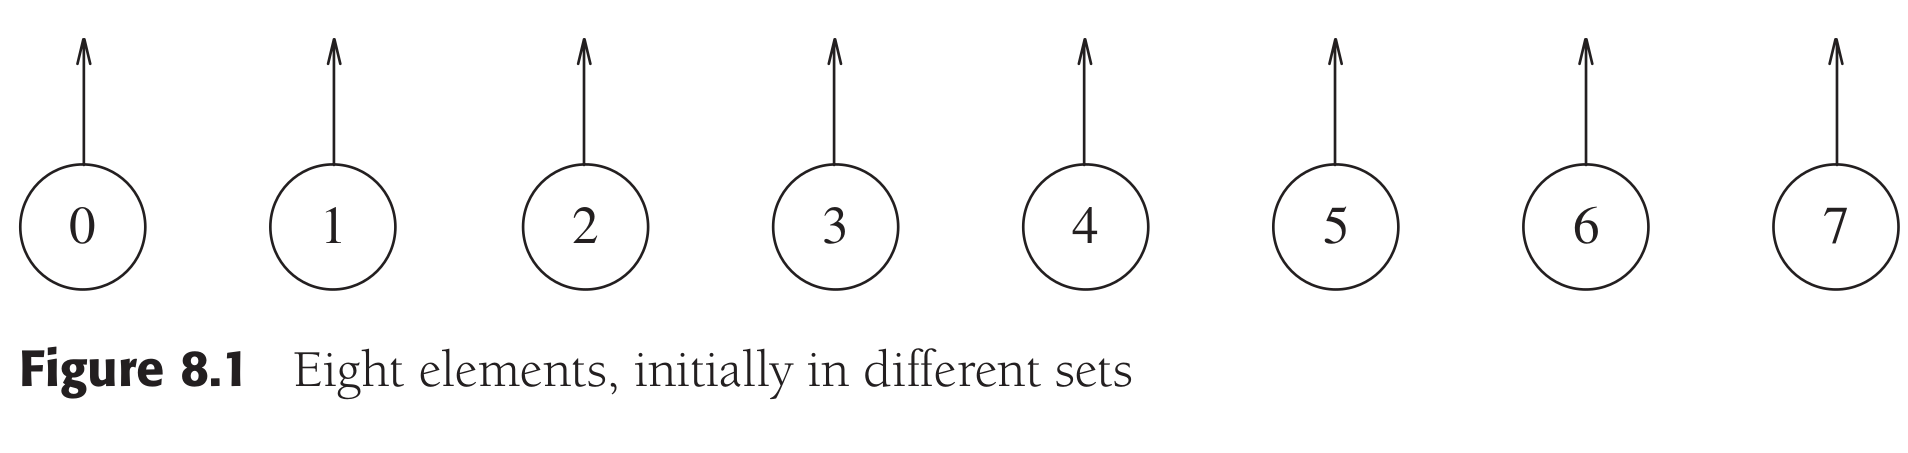
\includegraphics[width=0.75\textwidth]{images/FIG8_1.png}
\end{center}
我们可以设置
\begin{lstlisting}
  for i = 0 to 7
    s[i] = -1;
\end{lstlisting}
现在当我们合并两个类时, 只需修改其中一个类的根节点就行了, 所以一定是常数时间的. 
比如 Figure 8.2 中的合并是 \verb|union(4, 5)|, 
\begin{center}
  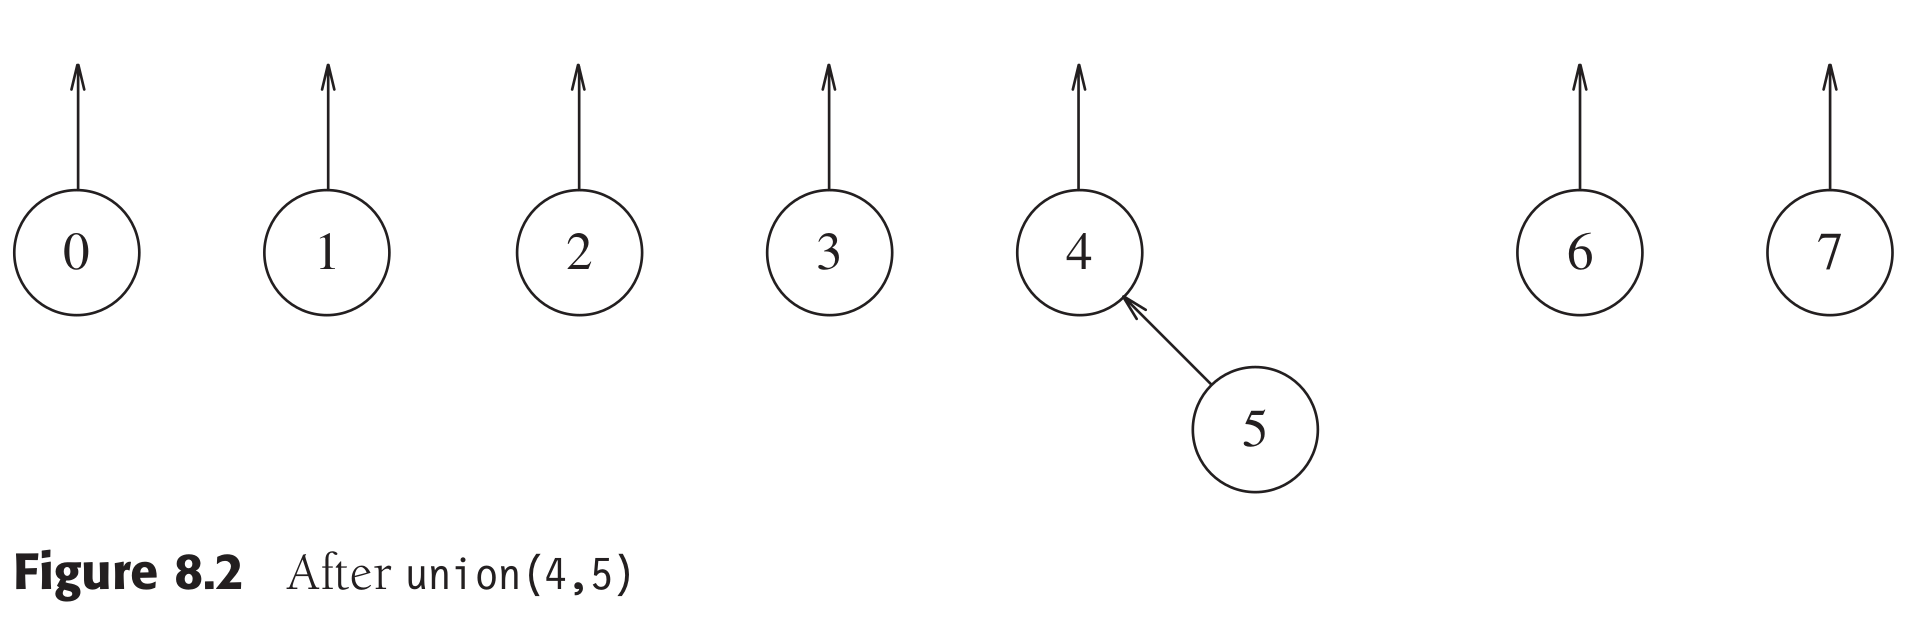
\includegraphics[width=0.75\textwidth]{images/FIG8_2.png}
\end{center}
那么体现在数据结构中就是 
\begin{lstlisting}
  s[5] = 4;
\end{lstlisting}
这里我们实际采用了向左合并原则, 也就是
\begin{lstlisting}
  union(x, y)
  s[y] = x;
\end{lstlisting}
往左边的参数合并. 这种方式显然不是最优的, 但易于实现.
Figure 8.3 中的 \verb|union(6, 7)|, 
\begin{center}
  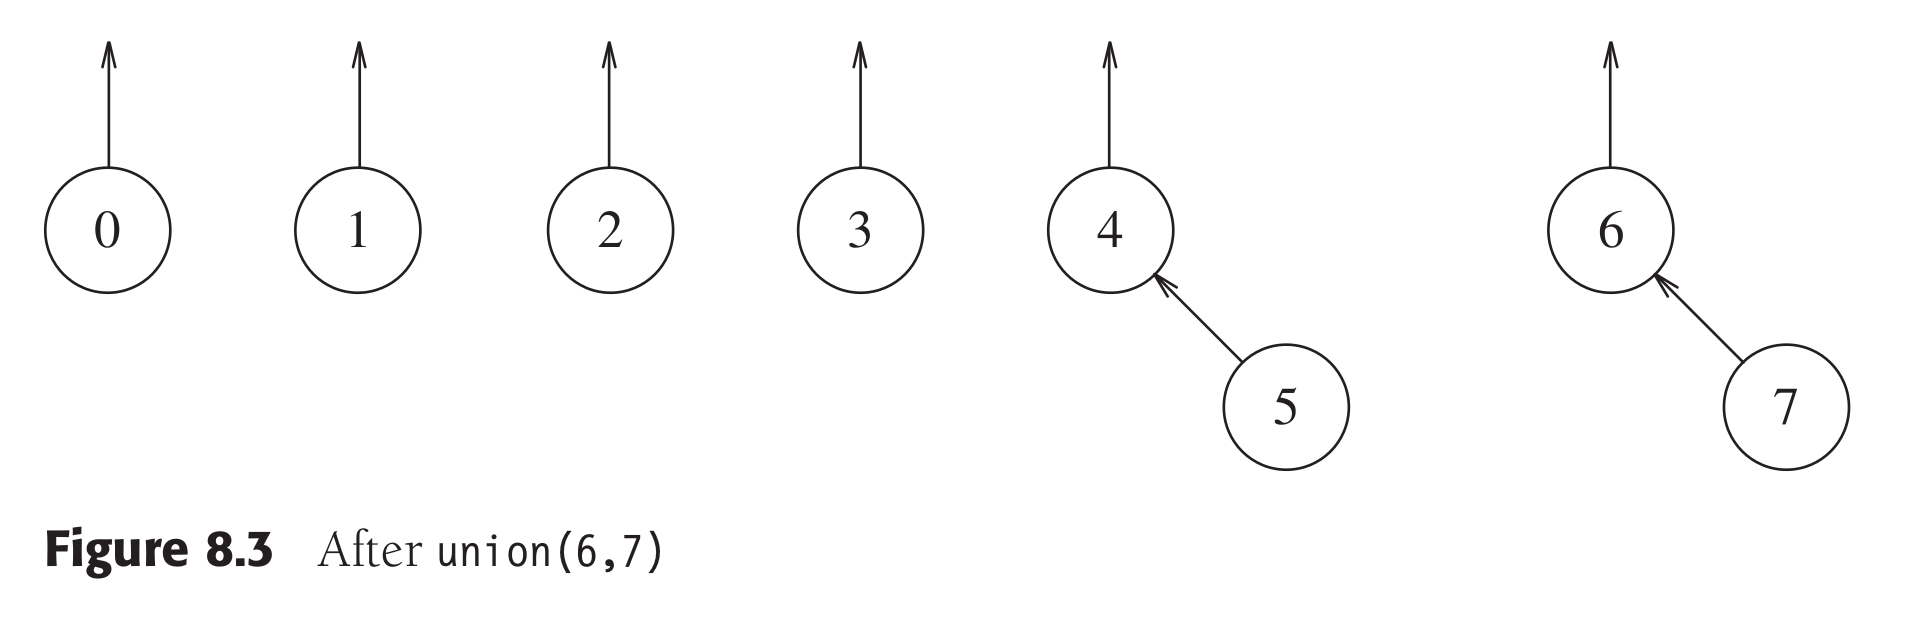
\includegraphics[width=0.75\textwidth]{images/FIG8_3.png}
\end{center}
就是
\begin{lstlisting}
  s[7] = 6;
\end{lstlisting}
Figure 8.4 中的 \verb|union(4, 6)|, 
\begin{center}
  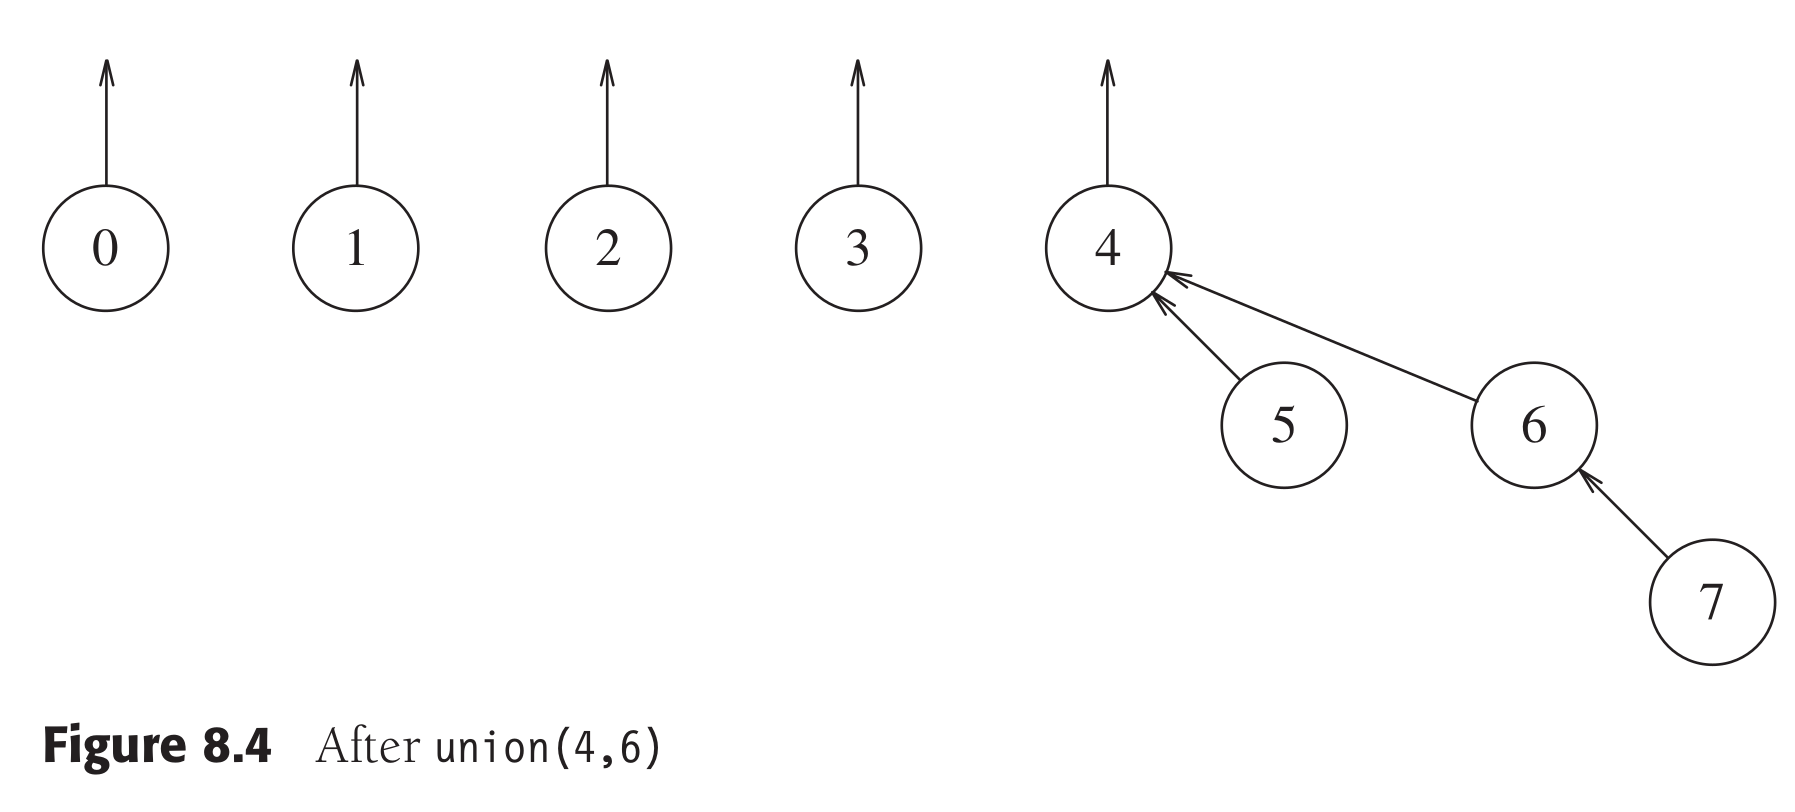
\includegraphics[width=0.75\textwidth]{images/FIG8_4.png}
\end{center}
就是
\begin{lstlisting}
  s[6] = 4;  
\end{lstlisting}
Figure 8.5 显示了上述操作结束之后的 \verb|s| 数组内容:
\begin{lstlisting}
  s|0 |1 |2 |3 |4 |5|6|7|
  -|-1|-1|-1|-1|-1|4|4|6|    
\end{lstlisting}

现在 \verb|find| 操作只需返回这个元素的根节点就是了, 也就是说跳转次数是树高. 
然而, 在最坏情况下, 树高是有可能为 $\Theta(N)$ 的 (全部合并成一个类, 且总是向左合并). 
显然, 我们需要对树高有所控制, 这就是为什么前面提出要小的类向大的类合并的理由. 
在目前情况下, 复杂度为对元素为 $N$ 的集合的连续 $M$ 个操作, 
最坏可能性下代价为 $\Theta(M N)$. 

以上操作具体的代码我们可以参考课本 Figure 8.6 ~ Figure 8.9. 并不难实现.

\subsection{更好的合并策略}

对合并策略的一个改进思路我们已经提到了, 就是小的类往大的类合并. 
这就要求我们跟踪类中的元素个数, 所以被称为 union-by-size. 
如果两个合并的类具有相同的大小, 那么我们仍然可以继续使用 ``靠左'' 的规则. 
所以我们的例子中的前三次合并和 union-by-size 策略并不矛盾. 
然后我们考虑操作 \verb|union(3,4)|, 
这个结果就是 Figure 8.10 中显示的. 
\begin{center}
  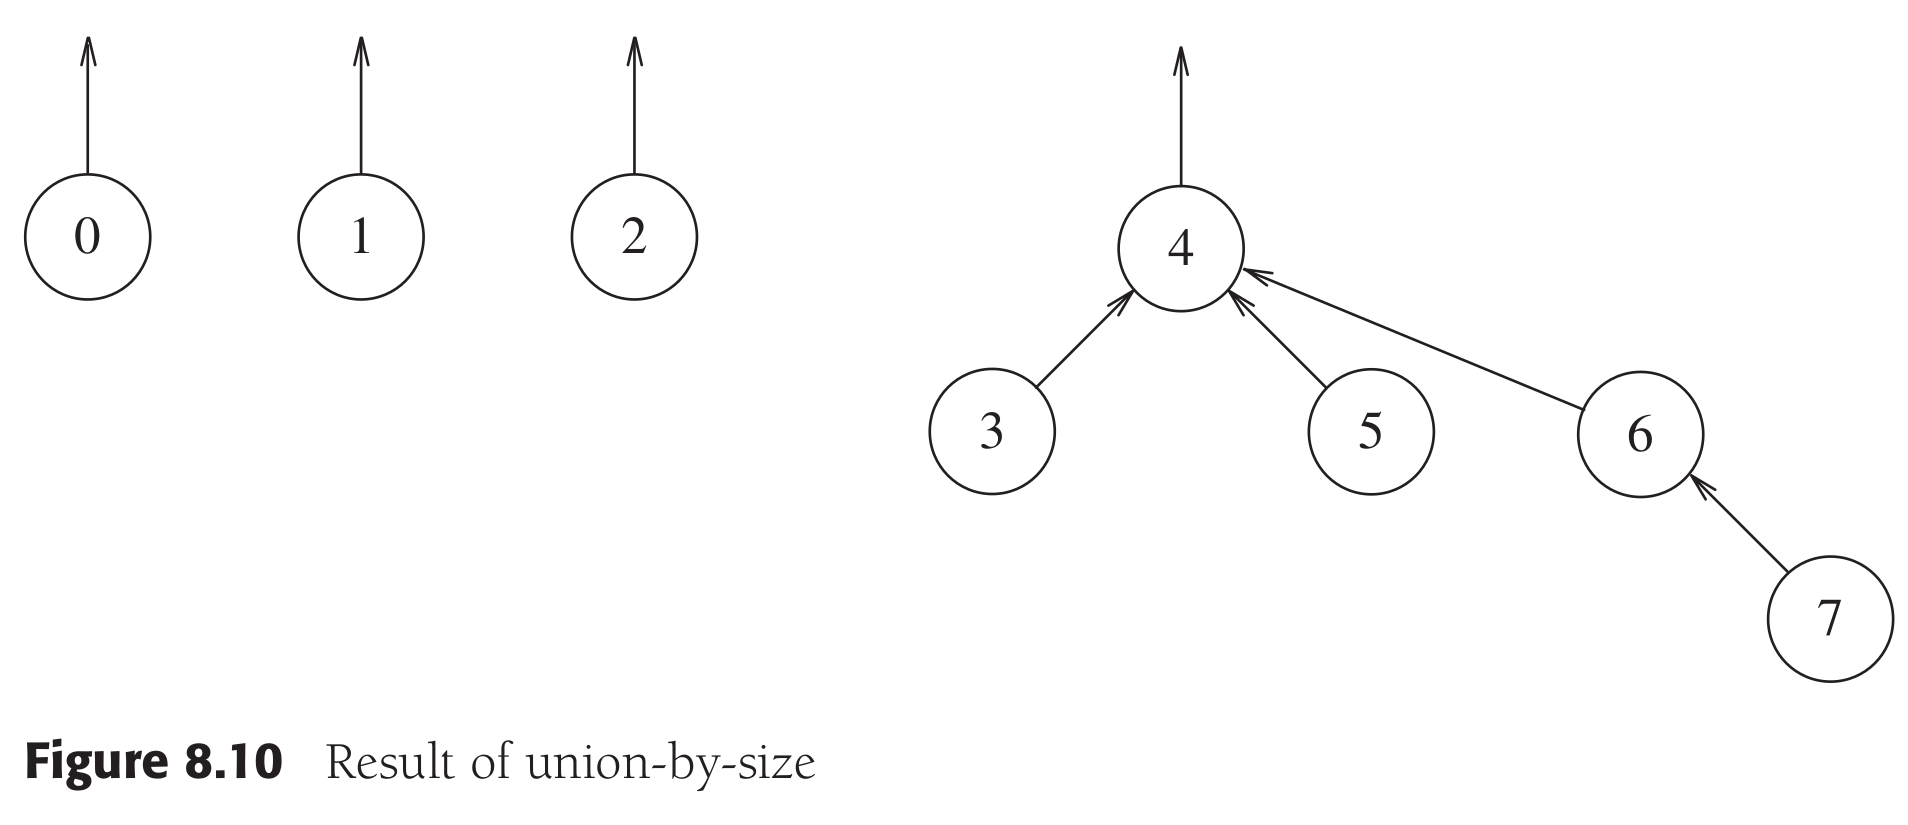
\includegraphics[width=0.75\textwidth]{images/FIG8_10.png}
\end{center}
我们注意到, 如果不采用 union-by-size, 
那么得到树就会开始加深. 也就是 Figure 8.11 的结果. 
\begin{center}
  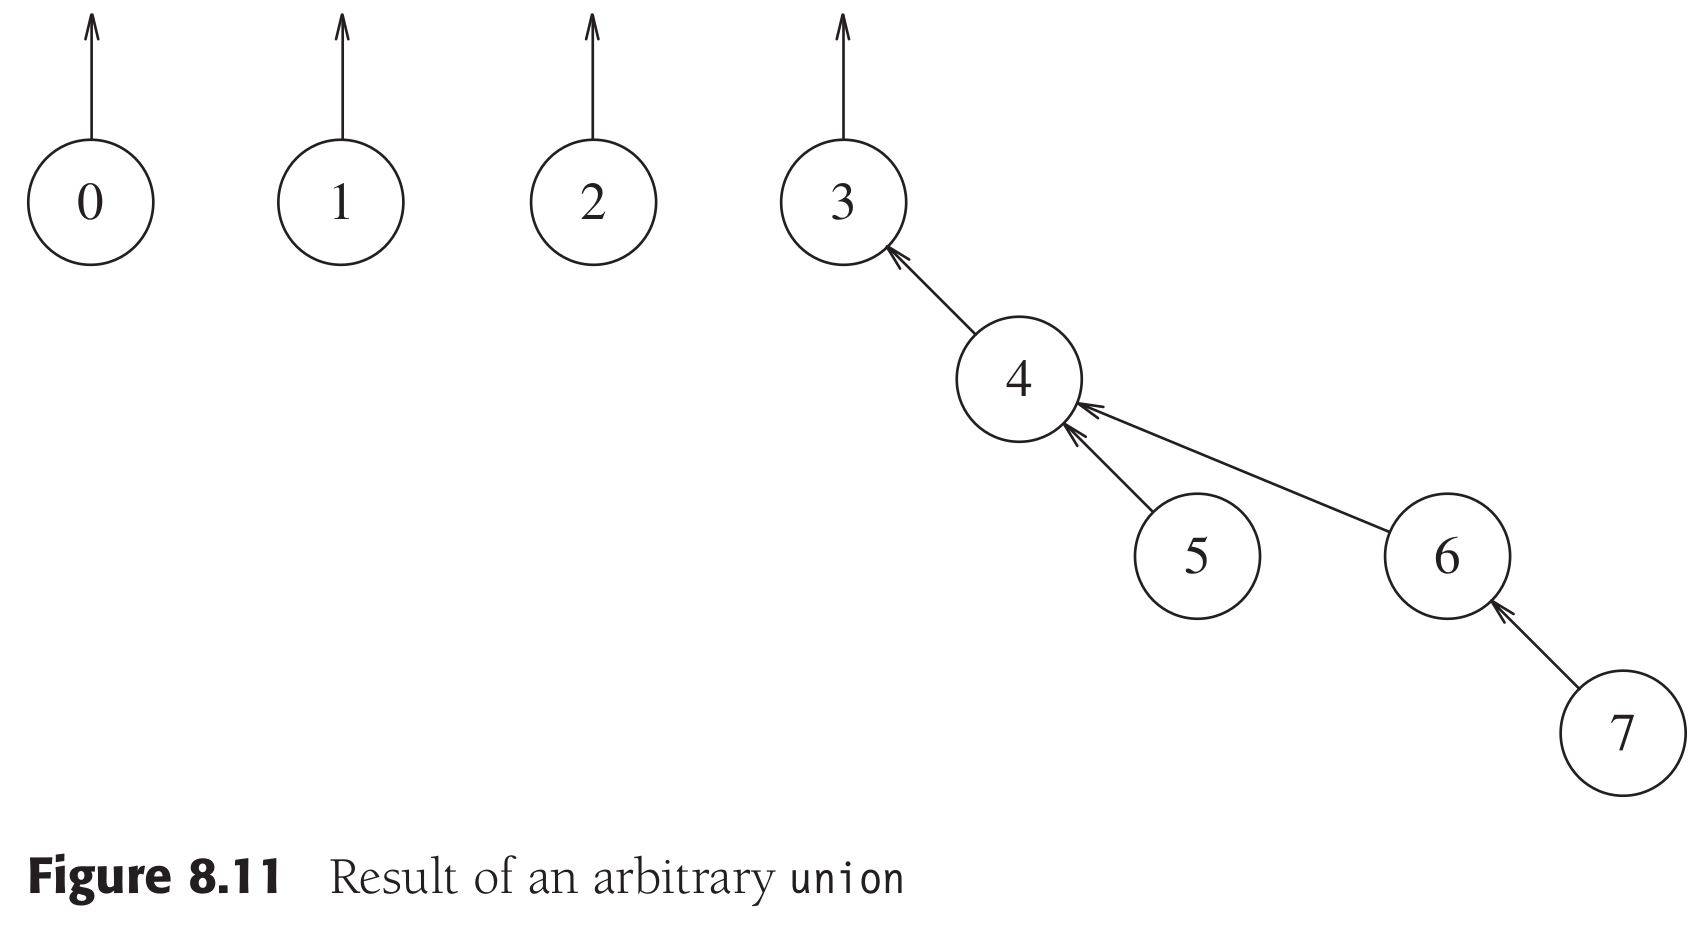
\includegraphics[width=0.75\textwidth]{images/FIG8_11.png}
\end{center}
不难证明, 采用了这个策略以后, 树的高度不会超过 $\log N$. 
Figure 8.12 给出了 $16$ 个节点的最坏可能.
\begin{center}
  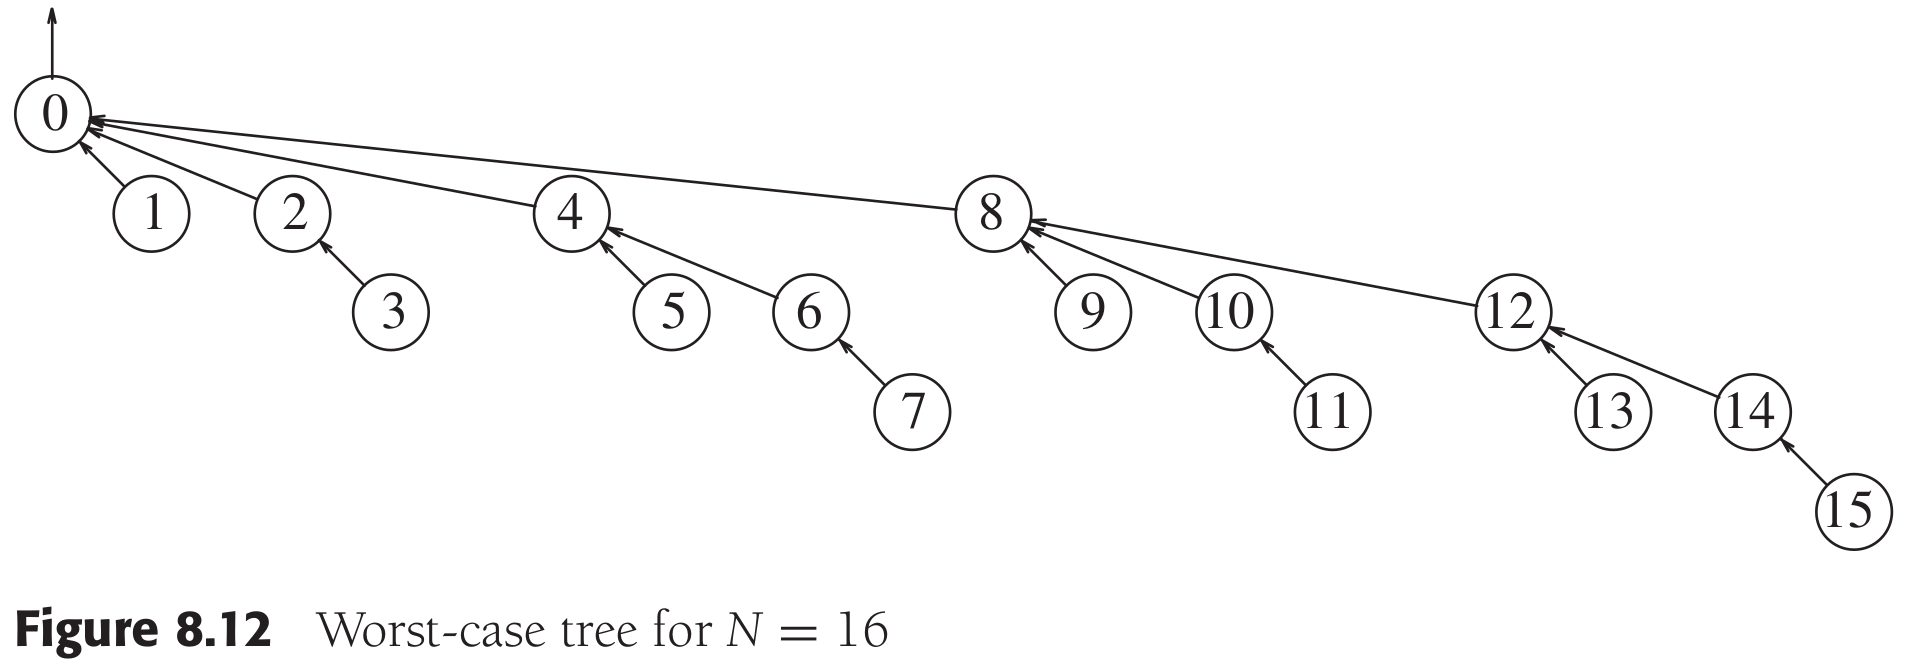
\includegraphics[width=0.75\textwidth]{images/FIG8_12.png}
\end{center}

而具体的实施时, 我们考虑到显然最合理存放树中元素个数的地方就是根节点. 
目前根节点只存放了一个信息量贫乏的 $-1$ 用来标志根, 着实浪费啊. 我们可以保持其值为负数, 
用以表达根的信息, 但是可以存放为 \verb|-size|, \verb|size| 是树中元素的个数. 
这样不但能直接读取树的元素个数, 还能直接通过两个根节点的比较来判定哪个数是更大的树. 

另一个可以考虑的策略是直接控制树的高度. 也就是我们直接在根节点记录 \verb|-height|, \verb|height| 是树的高度, 
合并的时候自然是从矮的向高的合并. 这个高度的维护比节点维护更容易的, 
因为高度发生变化的唯一情况就是两棵一样高的树合并, 合并之后的高度加 $1$. 
这种策略可以称为 union-by-height. Figure 8.13 显示了同一个操作,
\begin{center}
  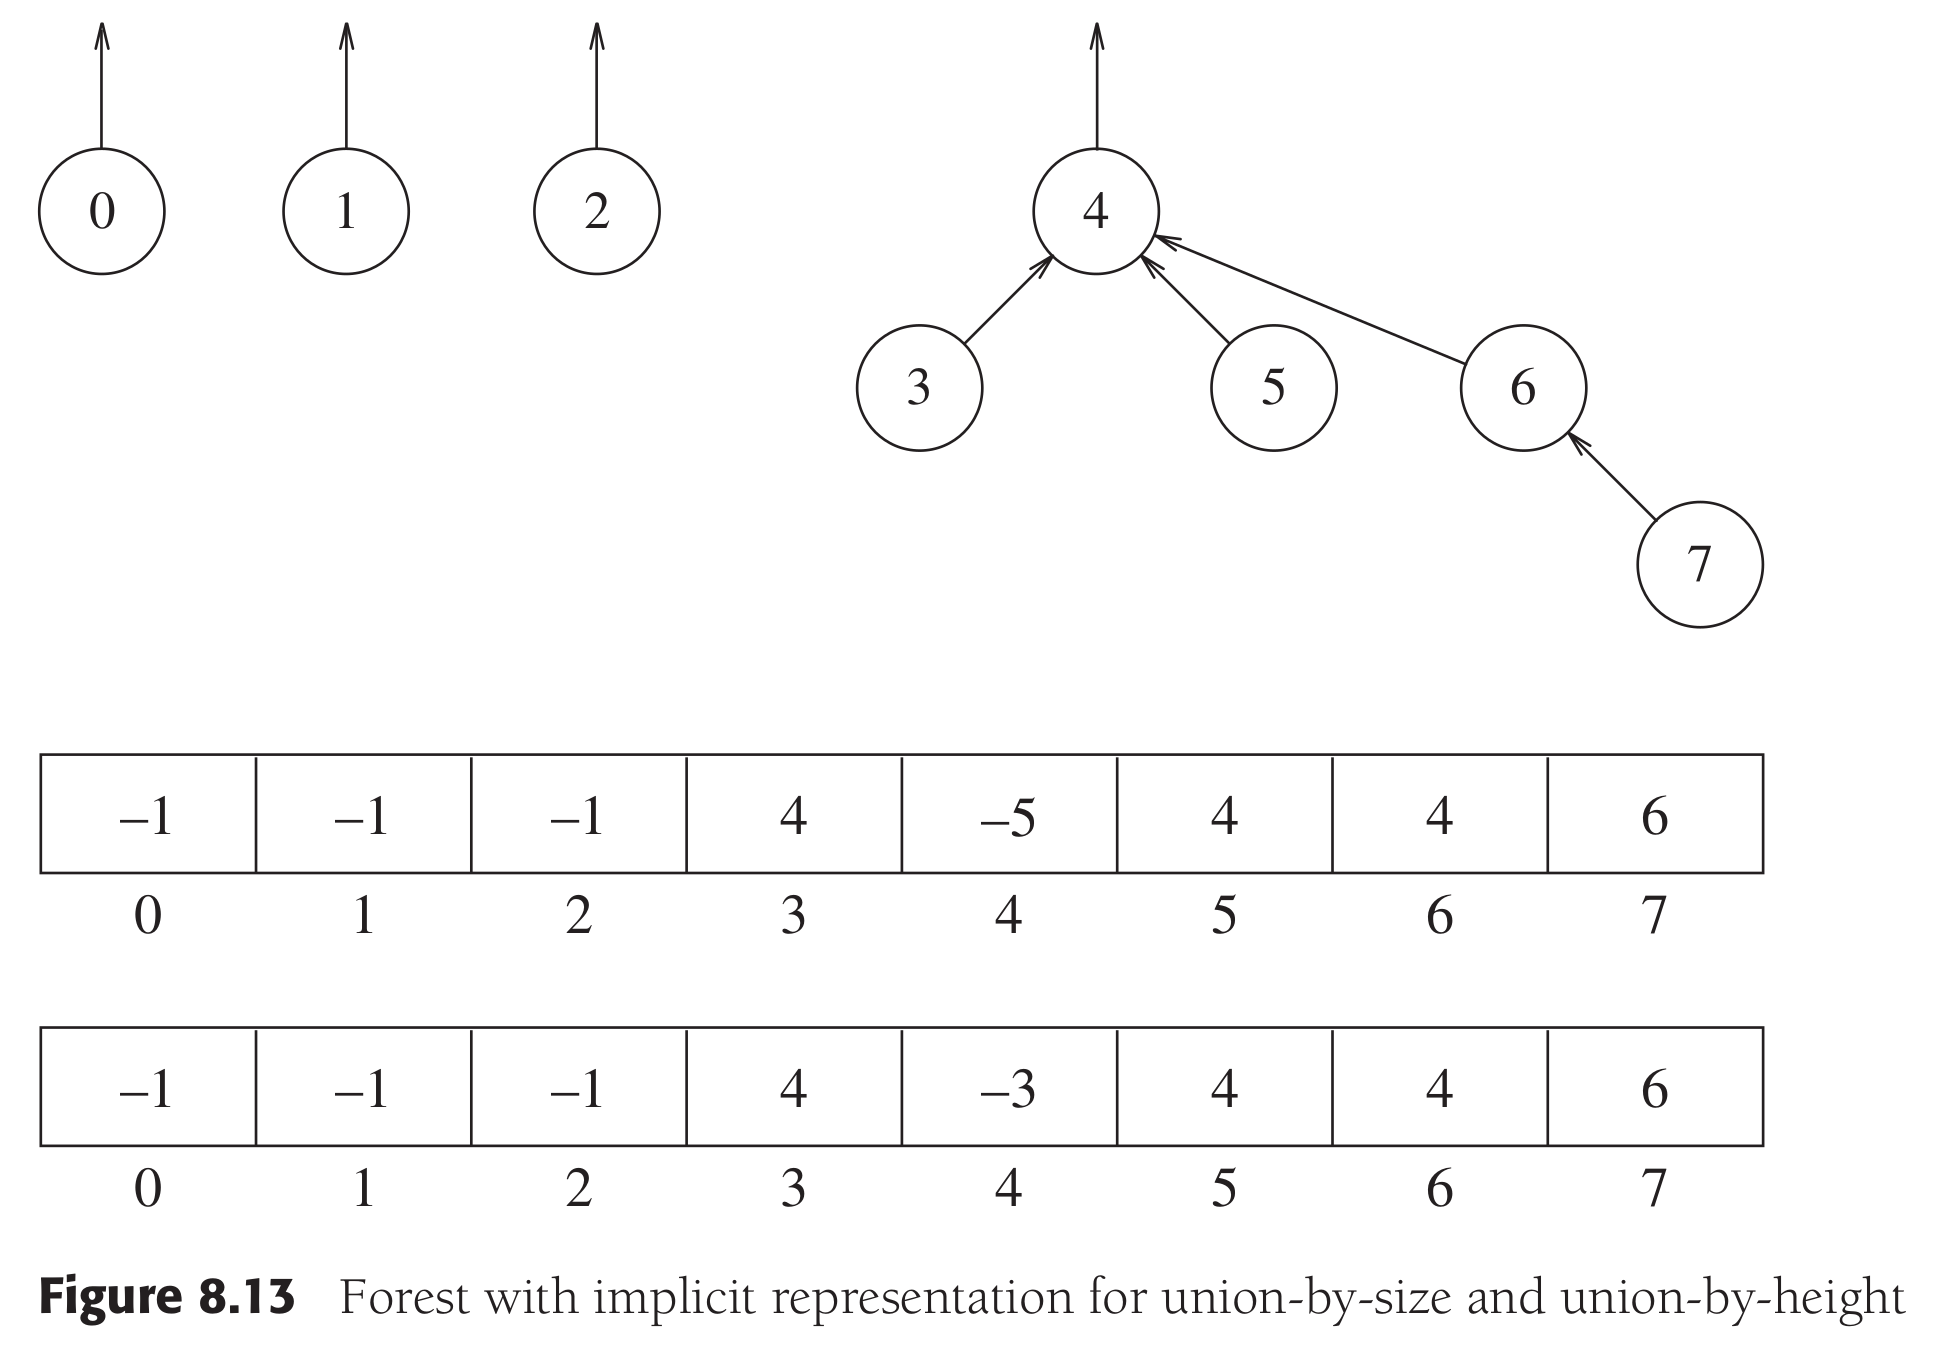
\includegraphics[width=0.75\textwidth]{images/FIG8_13.png}
\end{center} 
在 union-by-size 和 union-by-height 之后的区别. 
这个策略的代码实现是 Figure 8.14, 也不难.

\subsection{路径压缩}

之前的策略在大多数情况下可以运行良好. 但是, 对于查找次数远多于合并的情形, 
它的效率则不如最简单的数组实现. 因为在那个情形, 查找都是常数操作. 
可以认为, 合并已经不太有改进空间了, 但是我们仍然可以设法改进查找操作. 

这个想法也很简单, 就是每一次完成 \verb|find(x)| 操作之后, 都把 \verb|x| 的父节点改为这个类的根节点. 
从而显著地提升未来对 \verb|x| 及其后继节点的查找效率. 
而且这个操作可以在动态过程中不断改进. Figure 8.15 显示了 Figure 8.12 
中的树在一次 \verb|find(14)| 之后的变化. 
\begin{center}
  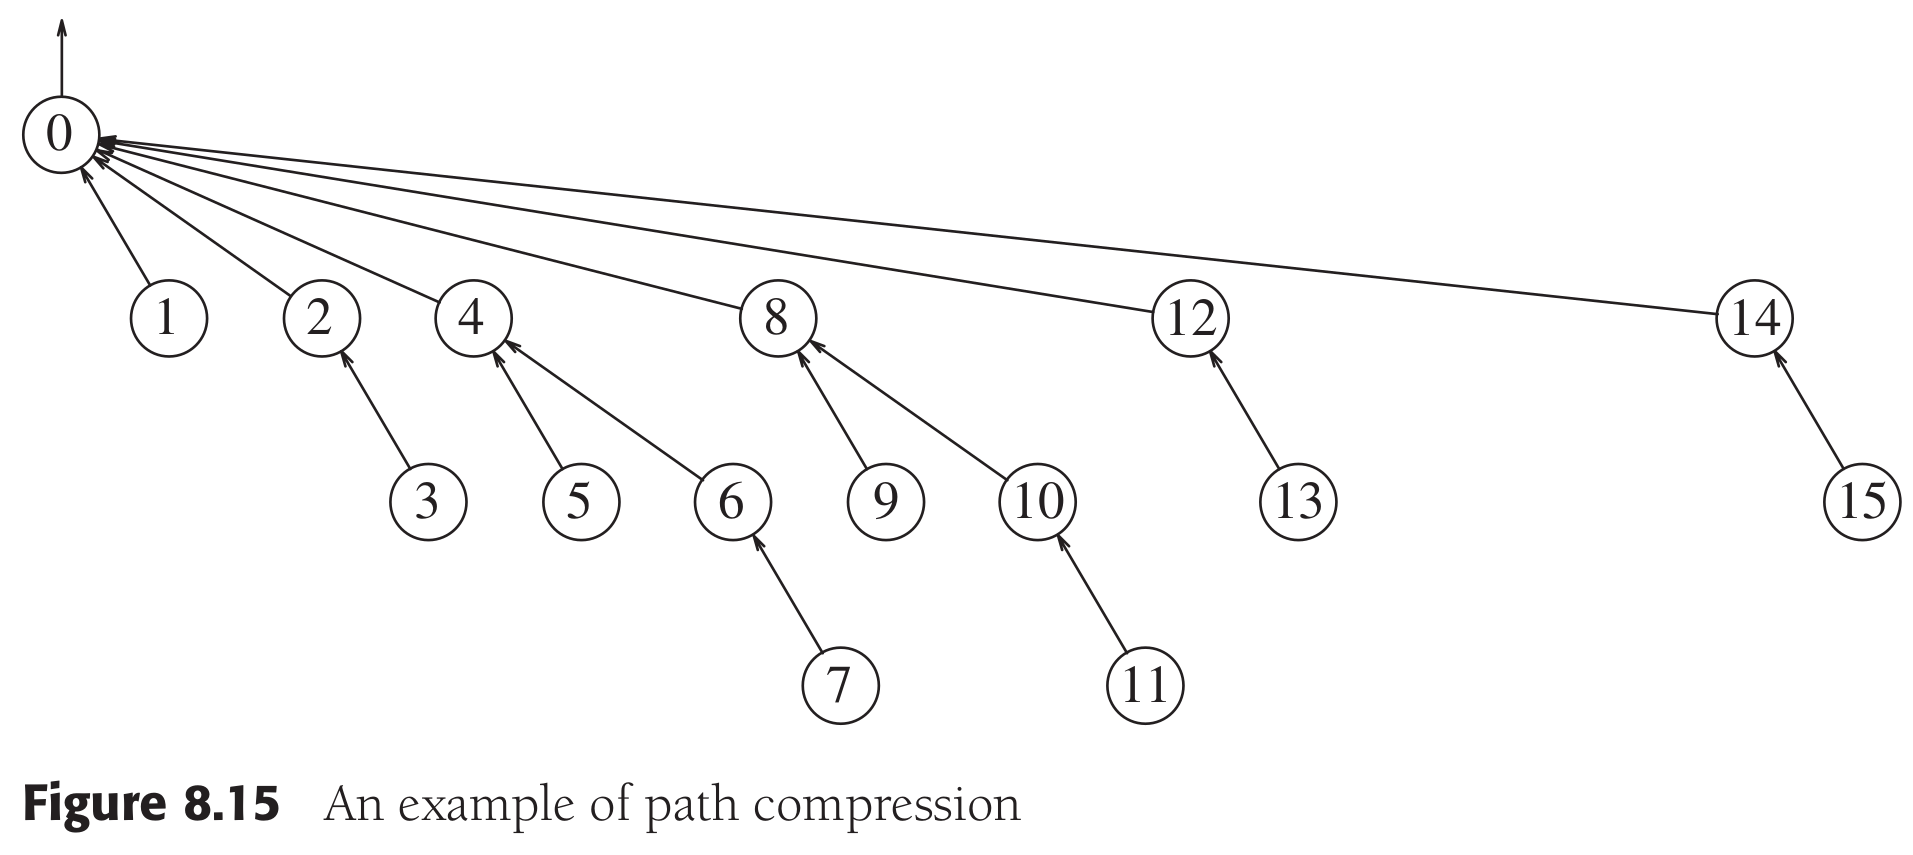
\includegraphics[width=0.75\textwidth]{images/FIG8_15.png}
\end{center} 
这个被称为路径压缩的策略在代码实现上也非常简单, 
参见 Figure 8.16. 它的一个较为重大的影响就是 \verb|find| 过程不再是一个静态过程, 而是会对结构作出修改.  

原则上, 查找中增加路径压缩是和合并相互独立的过程, 也就是理论上任何合并过程, 
在采用了路径压缩过程之后都可以显著地改善后续查找效率. 但是在具体实现中, 
union-by-size 是完全兼容这一策略的, 然而 union-by-height 则不是. 
原因很简单. 查找会导致树的结构发生变化, 同时也会影响可能不止一棵树的高度变化. 
是否应该, 已经如何高效率地更新这些树的高度, 是一个公开问题. 实际上, 
查找/合并问题本身的时间复杂度也是一个公开问题. 所以, 一个建议是, 不要去搜索改变这些树的高度值. 
于是这些根节点上存储的高度值, 逐渐就不再是真正的高度, 而只是一种优先度 (rank), 
于是, 这种合并策略就改名为 union-by-rank.

\subsection{应用: 迷宫的生成}
我们跳过第 8.6 节的理论分析部分, 有兴趣的同学可以自己阅读. 
我们直接进入更有趣的环节: 如何利用并查集来产生迷宫. 注意这并不是唯一的迷宫生成算法, 
但效果确实不错. 我们的迷宫是一个 $m$ 行 $n$ 列的网格, 每个格子都顺序编了号, 就按书上的例子, 
从左到右从上到下依次为 $0$, $1$, $2$, $\cdots$, $m \times n - 1$. 
每个格子, 都被四面墙围住, 除了左上角编号为 $0$ 的格子的左墙和右下角编号为 $m \times n - 1$ 
的格子的右墙以外. 

现在我们随机选取一面内墙(即除了最外围一圈墙以外的任何一块墙), 它必然和两个格子相邻, 
如果这两个相邻的格子并不相通, 则将这堵墙拆掉. 如此重复, 直到:
\begin{enumerate}
  \item 左上角和右下角的格子有通路, 或者
  \item 全部的格子两两都有通路.
\end{enumerate}

一般来说, 第 2 条终止策略产生的迷宫更加具有迷惑性. 

这里, 两个格子是否等价的判定就是这两个格子是否相通. 
初始情况, 全部墙都在, 全部格子都是自成一类的. 然后每一次随机取墙, 
我们都需要查找墙两侧的格子是否属于同一类, 如果不是, 拆掉墙, 同时应该合并它们各自所属的类. 
由此并查过程和随机拆墙挂钩. 第 1 种终止策略要求当 $0$ 号和 $m \times n - 1$ 号格子是同一类时终止; 
而第 2 种终止策略就是要求全部格子都在一个类时再终止.

\bibliography{crazyfish.bib}

\end{document}
